\section{Analysis Methodology}
\label{sec:methodology}

Charged particles traversing the TPC leave traces of ionisation electrons, which are drifted to the anode, composed of the three wire planes. The planes have 3 mm wire spacing at angles of $+60^{\circ}$, $-60^{\circ}$, and $0^{\circ}$ with respect to the vertical. The first two planes are referred to as \emph{induction planes} and the wire plane furthest from the cathode is referred to as the \emph{collection plane}. The planes are separated by 3~mm. Signal processing and noise suppression are extensively described in \cite{noise}. The waveforms observed on each wire are examined and a hit-finding algorithm searches for local maxima and minima. A Gaussian distribution is fitted to each peak and hits are created. 
The hits are input to the Pandora multi-algorithm pattern recognition software \cite{pandora} which first runs a two-dimensional reconstruction in which hits are clustered together by a series of algorithms in each readout plane. The common coordinate to all three images is exploited by further algorithms to correlate features and perform three-dimensional reconstruction, identifying the 2D clusters that represent individual particles, and creating with them the final TPC reconstructed objects \cite{pandora2}. Further characterisation of these objects will present them as track-like or shower-like based on topological features.

MicroBooNE also benefits from an optical detection system, comprised of 32 photomultipliers tubes placed behind the anode plane, with a few-ns timing resolution. They detect the argon scintillation light produced by the neutrino interaction and it provides the TPC start time of the event.
Figure \ref{fig:evd} shows a simulated $\nu_{e}$ CC0$\pi$-Np event display of the collection plane with an electron and two protons in the final state, and the corresponding reconstructed shower and reconstructed tracks. In this case, the algorithm is able to correctly identify the electromagnetic shower and both proton tracks.

\begin{figure}[htbp]
	\begin{center}
    	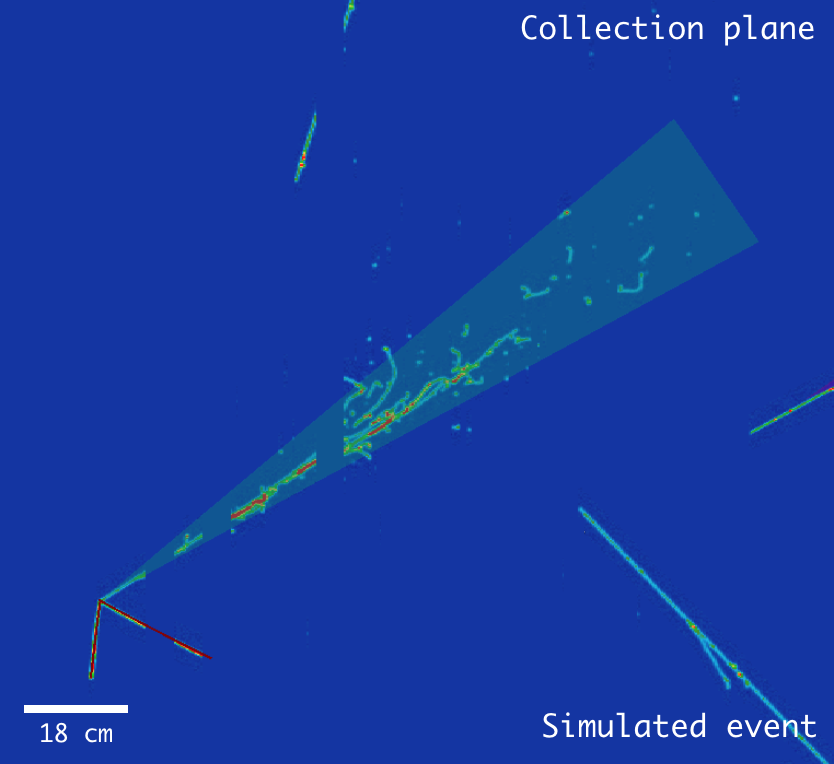
\includegraphics[width=0.5\linewidth]{figures/evd.png}
    	\caption{Monte Carlo $\nu_{e}$ CC0$\pi$-Np event display of the collection plane with an electron and two protons in the final state. The reconstructed shower-like object is represented by the green cone. The reconstructed track-like objects are represented by the red lines. The ionisation trails without an associated reconstructed track are cosmic rays correctly tagged by the cosmic removal algorithms. The colour scale is proportional to the amount of charge collected by the wires. {The vertical gaps are caused by the presence of missing or unresponsive wires in the detector, which are turned off in the simulation.}} \label{fig:evd}
	\end{center}
\end{figure}

\subsection{Data and Monte Carlo samples}\label{sec:data}
In this note, we will analyse a sub-sample of the data collected by the detector between February and April 2016. This sub-sample corresponds to an exposure of the MicroBooNE detector of \num{4.34e19} POT. This is MicroBooNE's unblinded sample for reconstruction, event selection development, and performance measurement. The sample is statistically too small to be sensitive to a MiniBooNE-like low-energy excess signal. 
The entire dataset will be open once we are satisfied with the reconstruction, analysis chain, and future sensitivity estimates.

The data was collected in two different modes, obtaining two different samples:
\begin{description}
\item[Data on-beam.] Each event was triggered in the detector by a flash in the optical detection system during the beam gate window, with the beam on;
\item[Data off-beam.] Each event was triggered in the detector by a flash in the optical detection system during an artificial beam gate window in which the beam is actually off.
\end{description}

Two different Monte Carlo samples were produced:
\begin{description}
\item[$\nu_{e}$ CC0$\pi$-Np + cosmic sample.] Each event has a simulated $\nu_{e}$ CC0$\pi$-Np interaction in the MicroBooNE cryostat and simulated cosmic rays hitting the detector in the same readout window. {The interaction is defined as $\nu_{e}$ CC0$\pi$-Np if it has one electron, at least one proton, no photons, and no mesons (pions, kaons) above detection threshold. The start and end points of the protons and the start point of the electron are required to be contained within the fiducial volume, as defined in Section \ref{sec:precuts}};
\item[BNB + cosmic sample.] Each event has a simulated $\nu$ interaction inside the MicroBooNE cryostat, where the neutrino flavors are weighted according to the BNB neutrino flux composition, and simulated cosmic rays hitting the detector in the same readout window.
\item[Dirt sample] {Each event has a simulated $\nu$ interaction outside the MicroBooNE cryostat, where the neutrino flavors are weighted according to the BNB neutrino flux composition, and simulated cosmic rays hitting the detector in the same readout window.}
\end{description}

Neutrino events have been generated using the GENIE Neutrino Monte Carlo generator version 2.8.6 \cite{genie} and cosmic rays have been generated using the CORSIKA Monte Carlo generator version 7.4003 \cite{corsika}. Simulated secondary particle propagation utilises GEANT version 4.9.6 \cite{geant}, and detector response simulation and reconstruction employs LArSoft version 6.26.01.10 \cite{larsoft}.

\subsection{Overview}

The reconstruction and selection chain to identify $\nu_{e}$ CC0$\pi$-Np electron neutrino candidate events for this analysis is divided into several stages:
\begin{enumerate}

\item Cosmic-ray removal:  in order to suppress the cosmogenic background \cite{cosmic, mucs}, two different Pandora reconstruction paths run with different sets of algorithms \cite{pandora}, a first one optimised for the reconstruction of cosmic-ray muons, and a second one optimised for the reconstruction of neutrino interactions. In between both reconstruction paths, hits associated with objects deemed as cosmic-induced by several tagging algorithms, external to Pandora and described in \cite{ubxsec}, are removed from the event. The remaining hit collection provides the input to the Pandora neutrino reconstruction path, which outputs a list of candidate neutrinos.

\item Optical pre-cuts and flash-matching: a minimum amount of coincident photoelectrons in the optical detection system is required and at least one of the neutrino candidates provided by the Pandora framework must be compatible with the flash in the optical detection system.
\item Electron neutrino topological pre-selection: one of the neutrino candidates must be compatible with the topology of a $\nu_{e}$ CC0$\pi$-Np interaction. Rather than accepting strictly $N$ tracks and one shower, at least one track and at least one shower or at least two showers sharing a common vertex are accepted, due to the presence of split showers and split tracks. Multiple showers without reconstructed tracks are accepted due to a current track/shower identification inefficiency.

\item CC $\nu_{\mu}$ neutrino candidates removal: events tagged as CC $\nu_{\mu}$ neutrino candidates are rejected by an independent selection module \cite{ubxsec}. 
\item Background rejection through calorimetric, kinematic, and geometric cuts: $\nu_{e}$ CC0$\pi$-Np events can be further isolated by applying a suite of cuts on kinematic, geometric, and calorimetric variables. The electromagnetic showers initiated by an electron in the final state are isolated with a cut on the $dE/dx$ value and the proton tracks are selected with a cut on the $\chi^{2}$ score of their $dE/dx$ vs. residual range profile.
\item Energy spectrum reconstruction: the energy of the electron showers is measured with a calorimetric procedure, converting the collected charge into deposited energy, while the energy deposited by the proton tracks is calculated from the length of the reconstructed track. 
\end{enumerate}

\subsection{Optical Detection System Selection}\label{sec:optical_pre_cuts}
The optical selection serves two purposes: (1) it ensures that the optical flash which triggered the detector readout is compatible with the neutrino candidates from the Pandora neutrino-optimised reconstruction pass, and (2) it provides a way to discriminate between multiple Pandora neutrino candidate objects (most of which are of cosmic origin) by selecting the one most compatible with the flash in the optical detection system in time with the beam gate window.

The optical selection algorithm consists of three major stages:
\begin{enumerate}
\item cuts applied to optical properties of the reconstructed flash object (number of photoelectrons an TPC charge/PMT photoelectrons ratio);
\item cuts on the compatibility of the reconstructed flash with the Pandora neutrino candidate (position of the flash compared with the position of the centre of the collected charge);
\item the Pandora neutrino candidate which is most compatible with the flash is picked using a likelihood method.
\end{enumerate}

The effects of the optical selection have been studied in detail using the $\nu_{e}$ CC0$\pi$-Np + cosmic Monte Carlo sample.



\subsection{Electron Neutrino Topological Pre-Selection} \label{sec:topological_pre_selection}
A perfectly reconstruction of a $\nu_{e}$ CC0$\pi$-Np event in a LArTPC will produce as many reconstructed tracks as the number of protons above the detection threshold in the final state and a single reconstructed shower (the electron), sharing a common vertex. However, mis-reconstruction and mis-classification can significantly lower the selection efficiency. The current status of the event reconstruction, which depends on the quality of the event (e.g. the number of hits \cite{pandora}), affects the efficiency of selecting these events. For example, the presence of dead or unresponsive wires can damage the reconstruction by causing the splitting of an ionisation track or an electromagnetic shower into two distinct reconstructed object. Also, the selection currently implemented relies on the classification of the reconstructed objects as track-like or shower-like, separation that contains an inherent inefficiency associated, specially when the number of reconstructed hits is low.

In order to maximise our efficiency we currently require (1) \emph{at least} one track and \emph{at least} one shower sharing a common vertex, or (2) \emph{at least} two showers sharing a common vertex, to account for proton mis-classification as a shower-like object. For these cases we measure the $\chi^2$ score of the $dE/dx$ vs. residual range profile of the reconstructed objects in the proton hypothesis. The object with the lowest $\chi^2$ score is considered as a track, while the remaining ones are considered as showers.

\subsection{Minimum quality requirements}\label{sec:precuts}
A minimal set of cuts is applied to the selected events, in order to ensure that they are well reconstructed.
First, to avoid border effects, the reconstructed neutrino vertex, the start point of the reconstructed showers and the start and end points of the reconstructed tracks are required to lie within a fiducial volume. Our fiducial volume cut is 10~cm from each side on the $x$ axis, 15~cm from each side on the $y$ axis, and 10~cm (40~cm) from the upstream (downstream) side on the $z$ axis. 
Since electromagnetic showers develop mainly in the forward direction with respect to the beam, the asymmetric cut on the $z$ axis (which corresponds to the beam direction) helps reject non-fully contained events which begin too close to the downstream end of the TPC.
We also require, for each event, (1) at least 5 hits in the three planes associated to a shower-like object, (2) at least 5 hits in the three planes associated to a track-like object, and (3) at least one hit in every plane.


\subsection{Selection efficiency}\label{sec:eff}
The selection efficiency of our algorithm is obtained by calculating the fraction of events selected in the $\nu_{e}$ CC$0\pi$-Np + cosmic Monte Carlo sample, where the true neutrino vertex, the start and end points of the protons, and the start point of the electron are fully contained in the fiducial volume.

In order to understand what energy thresholds are appropriate for reconstruction in the TPC, dedicated studies have been performed on proton tracks and electron showers, using the $\nu_{e}$ CC$0\pi$-Np + cosmic Monte Carlo sample. We have found that we have no efficiency for reconstructing and classifying protons {with a kinetic energy} below 40~MeV and electrons{, photons, and charged pions} {with a kinetic energy} below 20~MeV following these optical, topological, and minimum quality pre-selections. Therefore, these energy thresholds are applied to the simulations to allow a fair comparison with the reconstructed particles. 

Our overall $\nu_{e}$ CC$0\pi$-Np selection efficiency $\epsilon$ is defined as:
\begin{equation}
\epsilon = \frac{\mathrm{N.~of~selected~}\nu_{e}\mathrm{~CC0}\pi\mathrm{{\text -}Np~events}}{\mathrm{N.~of~generated~}\nu_{e}\mathrm{~CC0}\pi\mathrm{{\text -}Np~events}},
\end{equation}
where each selected event must pass the optical selection, satisfy the topology and minimum quality requirements, and not being vetoed by the independent CC $\nu_{\mu}$ selection module. 


Figure \ref{fig:effpurity} shows the efficiency as a function of the true neutrino energy.
%The energy reconstruction procedure is described in section \ref{sec:energyreco}.
The systematic uncertainties related to the GENIE model and the neutrino beam flux are also included. The inner error bars represent the Monte Carlo statistical uncertainty, while the outer error bars are obtained summing in quadrature the statistical and the systematic uncertainties. 
As expected, the efficiency increases with the neutrino energy, since high-energy events correspond in general to a larger number of hits in the TPC and the Pandora framework reconstruction performances increase with the number of reconstructed hits \cite{pandora2}. 

A description of future improvements, which will allow us to increase the selection efficiency, is included in Section \ref{sec:future}.

% \todo{Add efficiency plots over a larger energy region for protons and electrons.}

\begin{figure}
\centering
%   \begin{subfigure}{0.48\textwidth}
    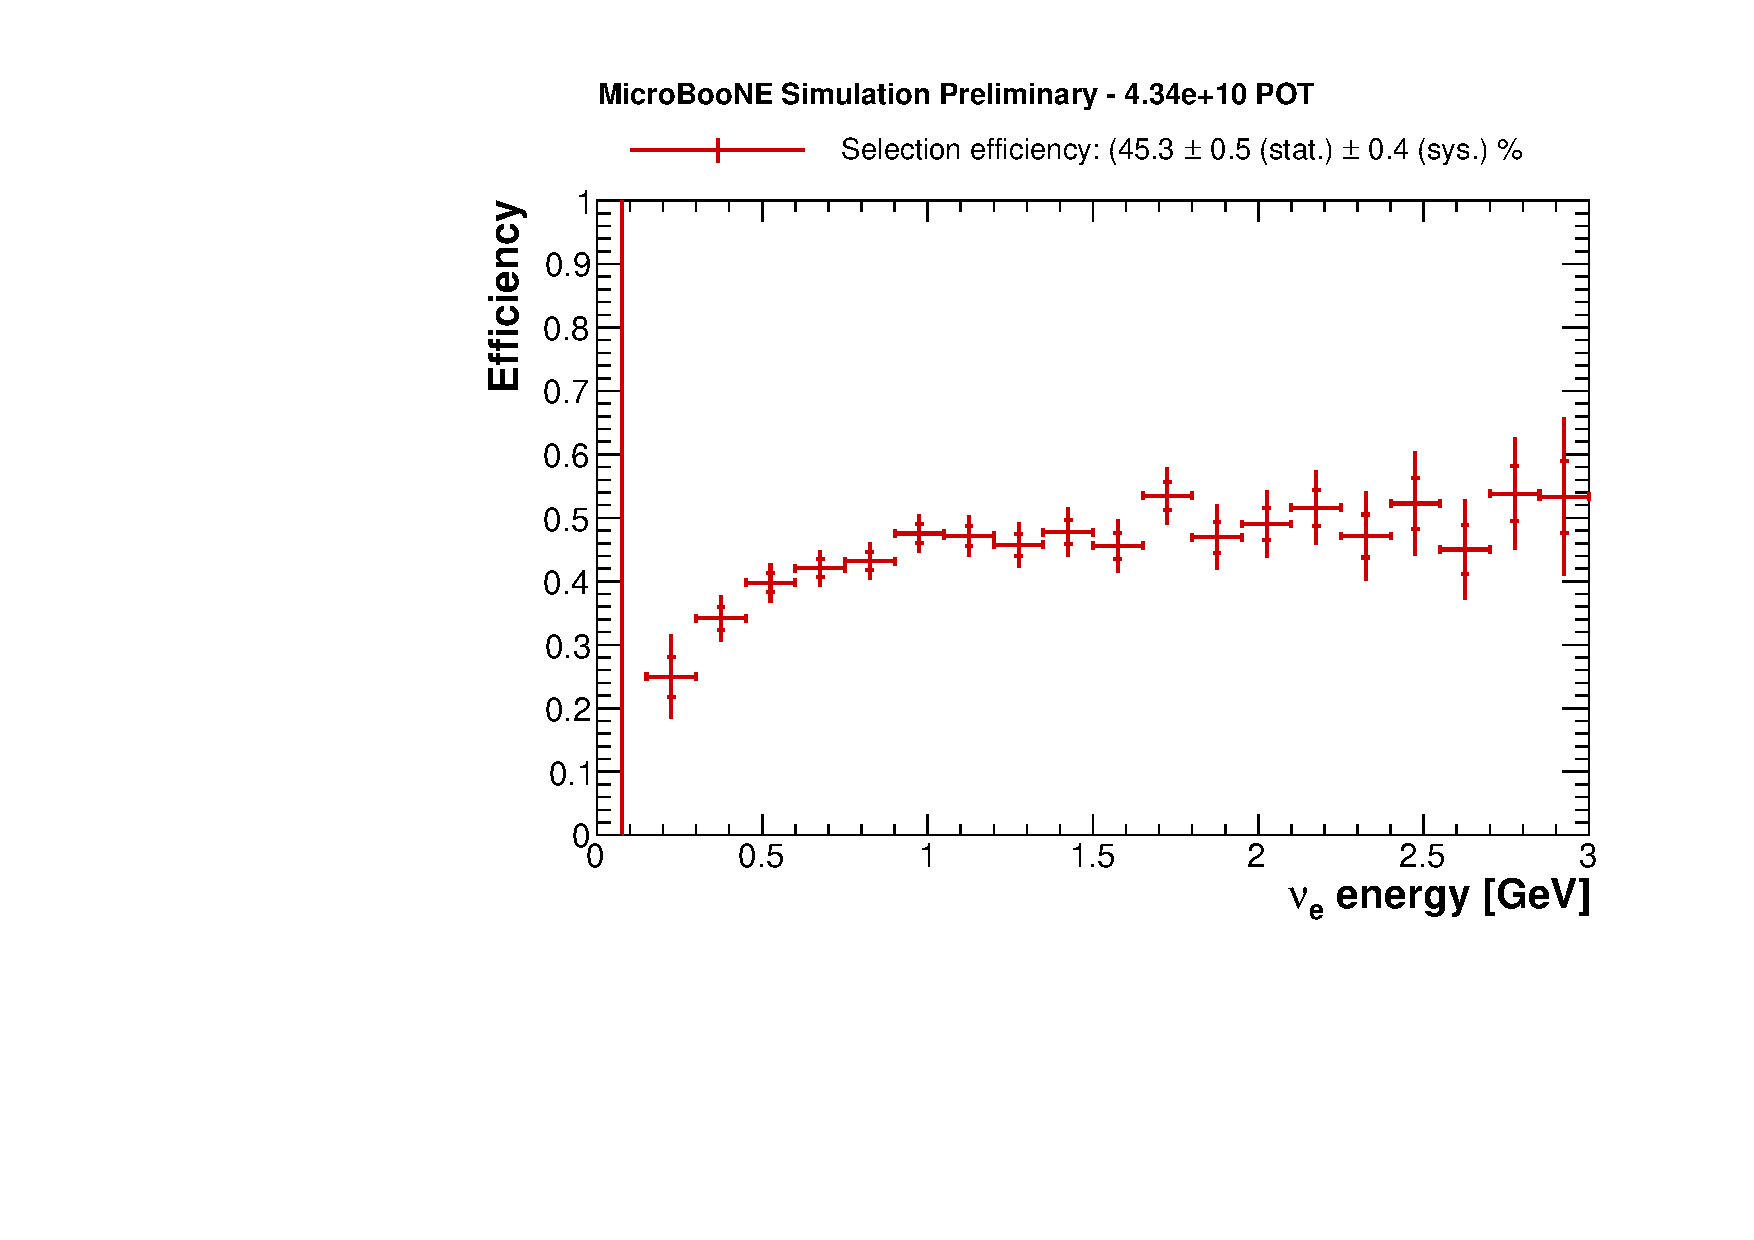
\includegraphics[width=0.65\linewidth]{figures/eff.pdf}
%     \caption{Efficiency.} 
%   \end{subfigure}
%     \begin{subfigure}{0.48\textwidth}
%     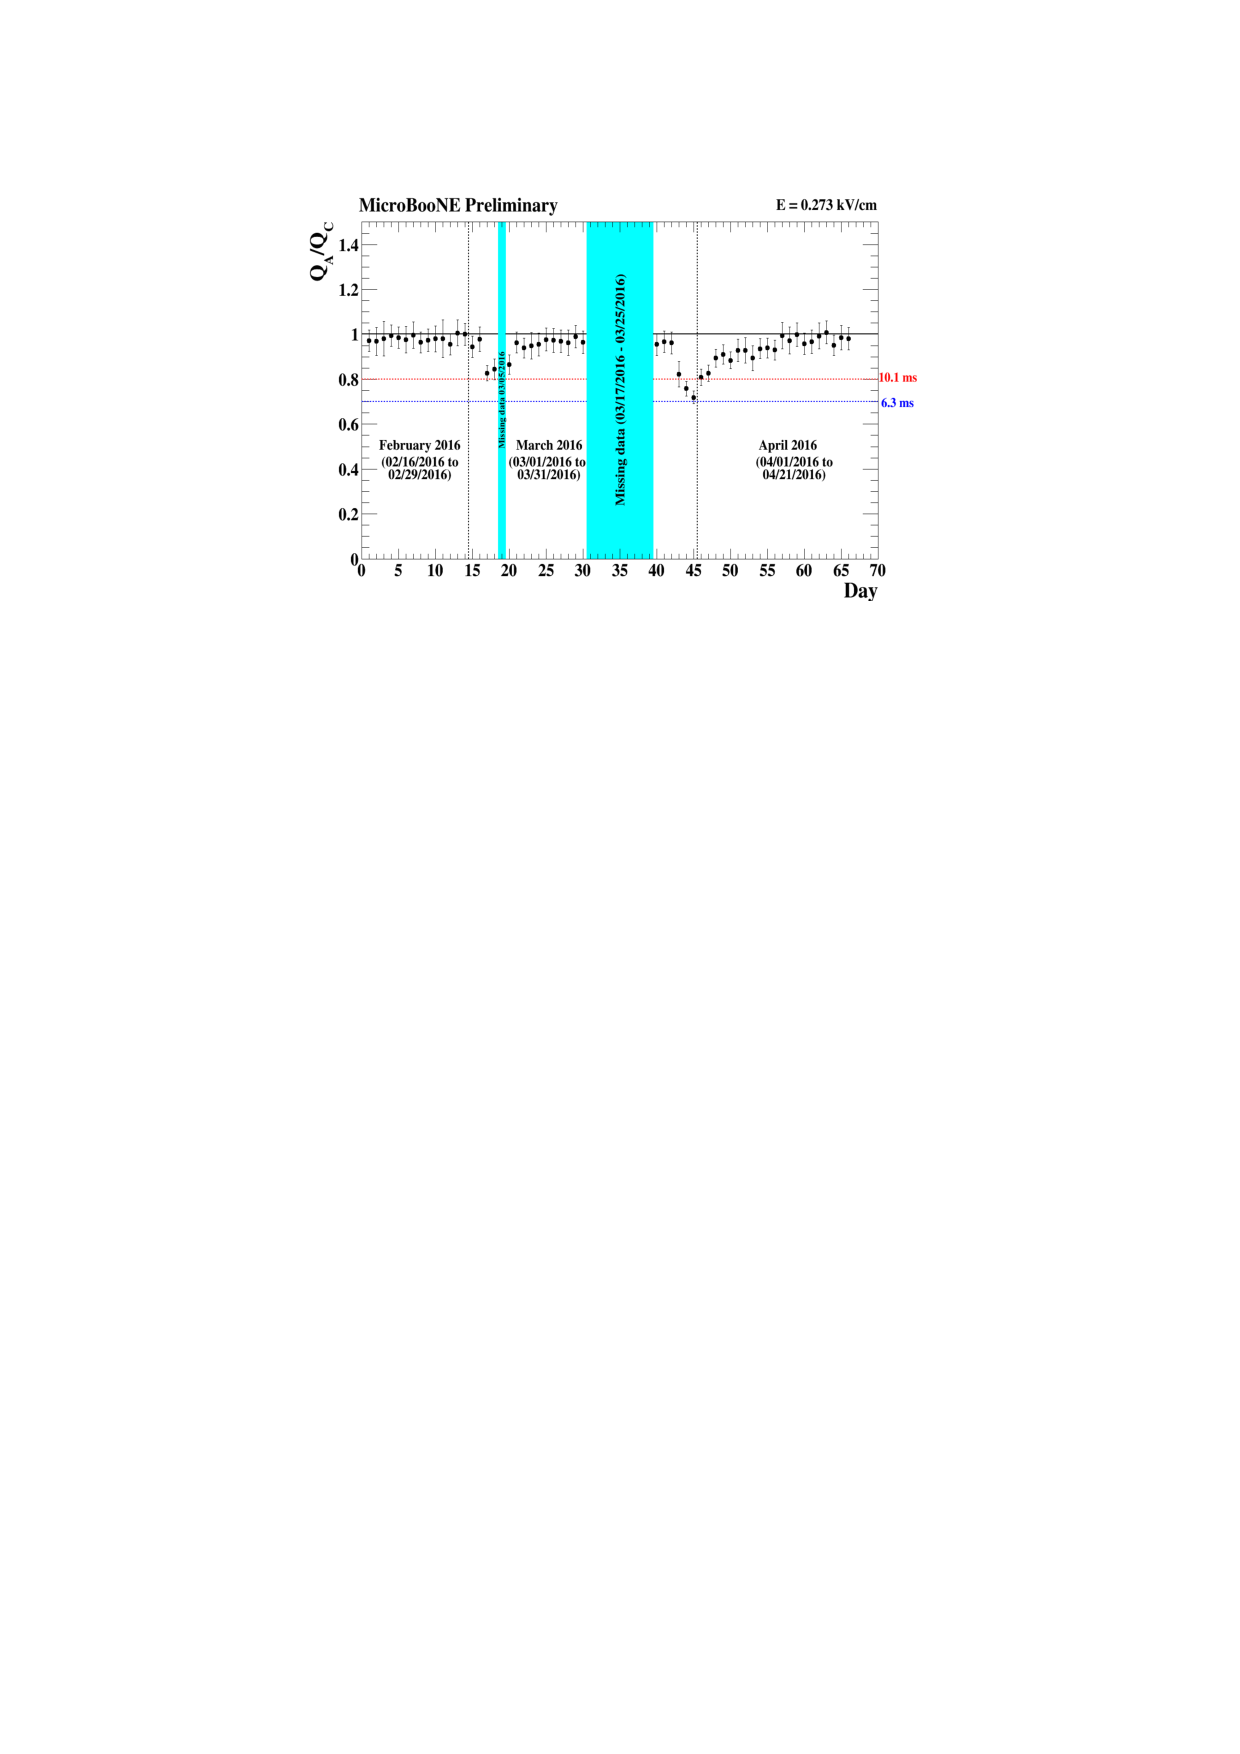
\includegraphics[width=\linewidth]{figures/purity.pdf}
%     \caption{Purity.} 
%   \end{subfigure}
  \caption{$\nu_{e}$ CC$0\pi$-Np selection efficiency as a function of the true $\nu_{e}$ energy. Each true proton (true electron) in the final state is required to have a kinetic energy larger than 40~MeV (20~MeV).}
  \label{fig:effpurity}
\end{figure}

\subsubsection{Inefficiencies breakdown}\label{sec:ineff}
Our current selection algorithm can fail for several reasons: in particular, we could have problems in the classification, such as an electron classified as a track-like object, or particles not reconstructed at all. We identified eight main causes for our selection inefficiency, whose contributions have been estimated with the same simulated sample described in Section \ref{sec:eff}:
\begin{description}

\item[Quality cuts (8.5\%).] {The selected neutrino candidate does not satisfy our minimum quality requirements, as described in Section \ref{sec:precuts}.}
\item[CC $\nu_{\mu}$ selected (4.2\%).]  {The event is tagged as a CC $\nu_{\mu}$ candidate by an independent selection module, described in \cite{ubxsec}}. 
\item[Not contained (10.5\%).] {One of the reconstructed tracks or the starting point of one of the reconstructed showers is not contained in the fiducial volume. As expected, this fraction increases with the neutrino energy}.
\item[Cosmic selected (8.5\%).] {The selected neutrino candidate has one or more reconstructed objects of cosmic origin}.
\item[1 shower (3.4\%).] {The selected neutrino candidate has only one associated reconstructed shower and no other object}. 
\item[No showers (13.5\%).]  {The selected neutrino candidate has only reconstructed track(s) associated. This is the largest contribution to the inefficiency, especially at low energies, since low-energy electrons are very challenging to reconstruct and classify as showers.}
\item[No flash (5.5\%).]  {The flash collected by the optical system does not satisfy our requirements, described in Section \ref{sec:optical_pre_cuts}}.
\item[No data products (0.7\%).] {The event does not have any neutrino candidate}.
\end{description}

Figure \ref{fig:ineff} shows a stacked histogram of the generated events, divided into the categories described above. The \emph{passed} category corresponds to the efficiency plot shown in Figure \ref{fig:effpurity}.

\begin{figure}
\centering
%   \begin{subfigure}{0.48\textwidth}
    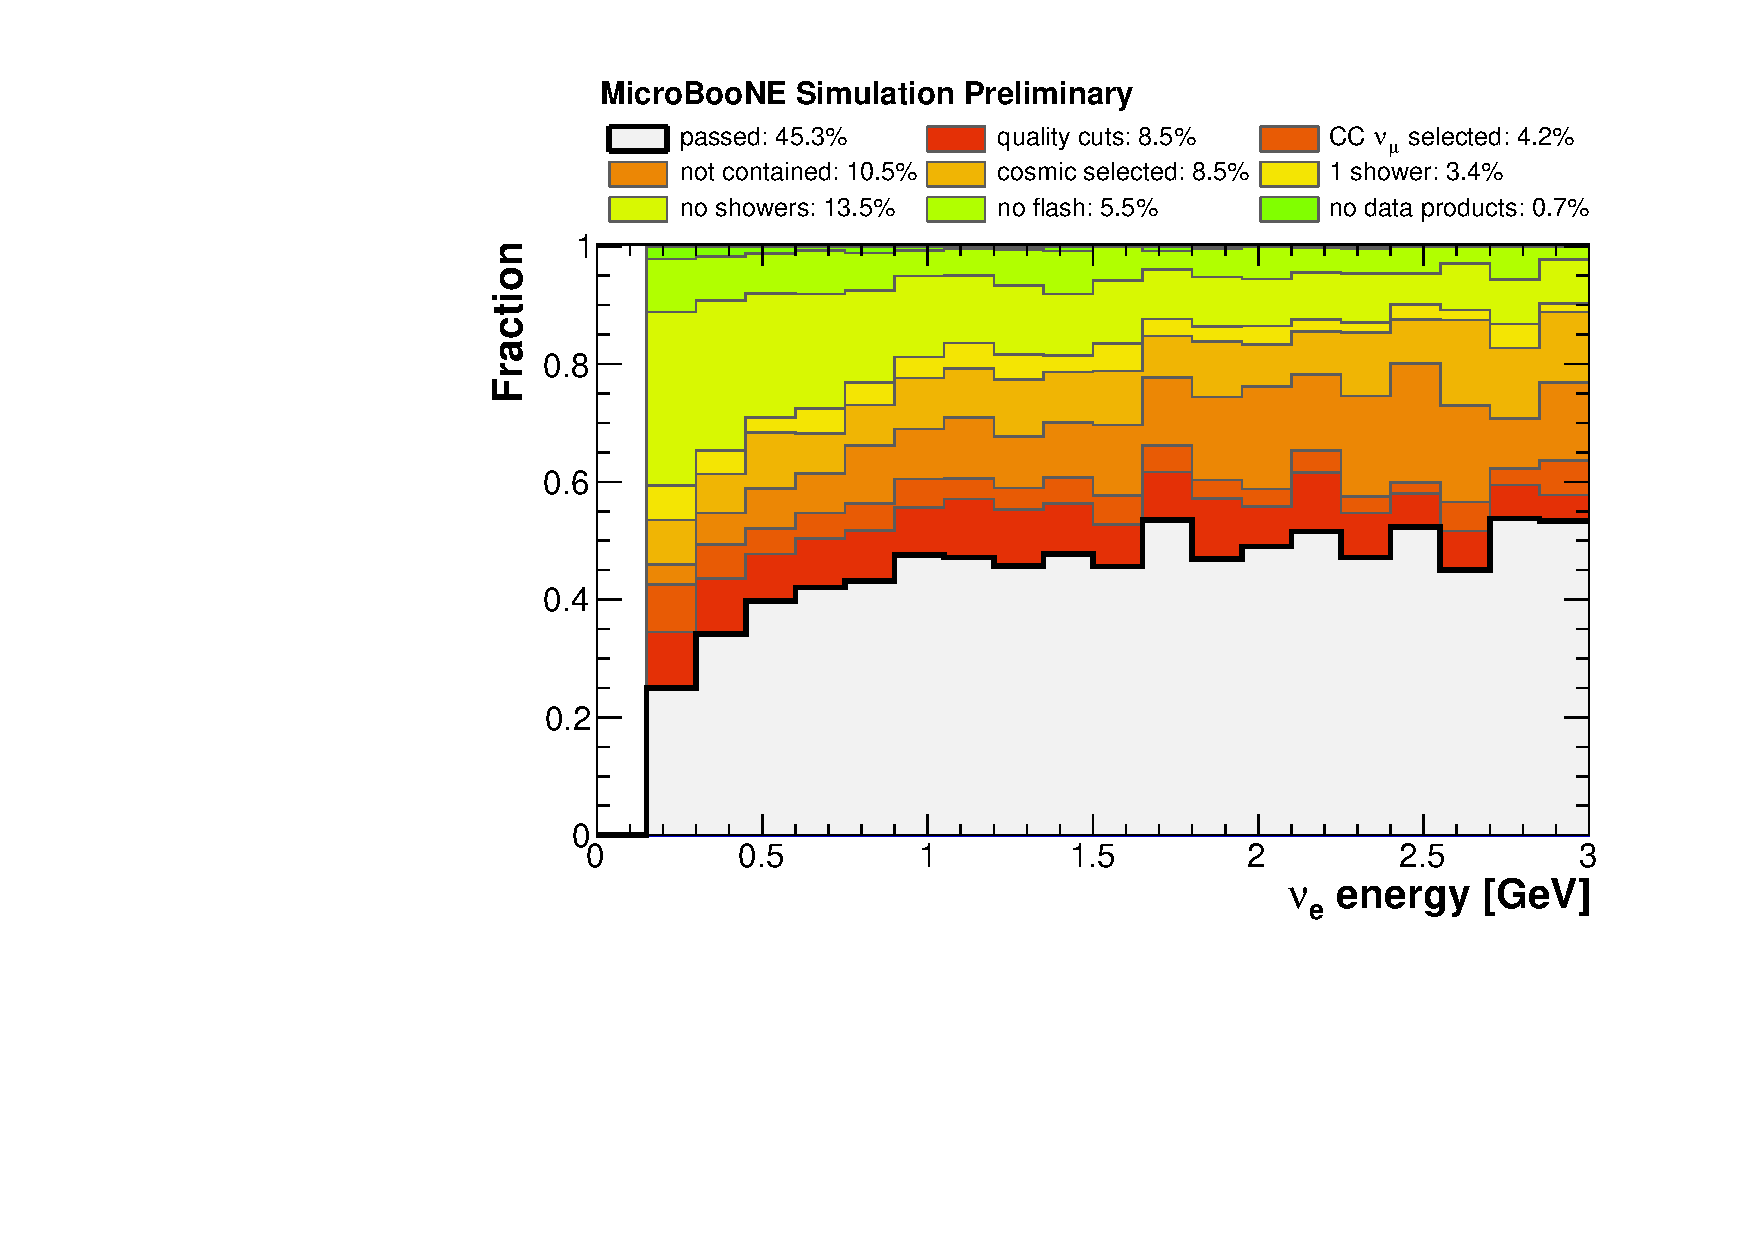
\includegraphics[width=0.65\linewidth]{figures/ineff.pdf}
%     \caption{Efficiency.} 
%   \end{subfigure}
%     \begin{subfigure}{0.48\textwidth}
%     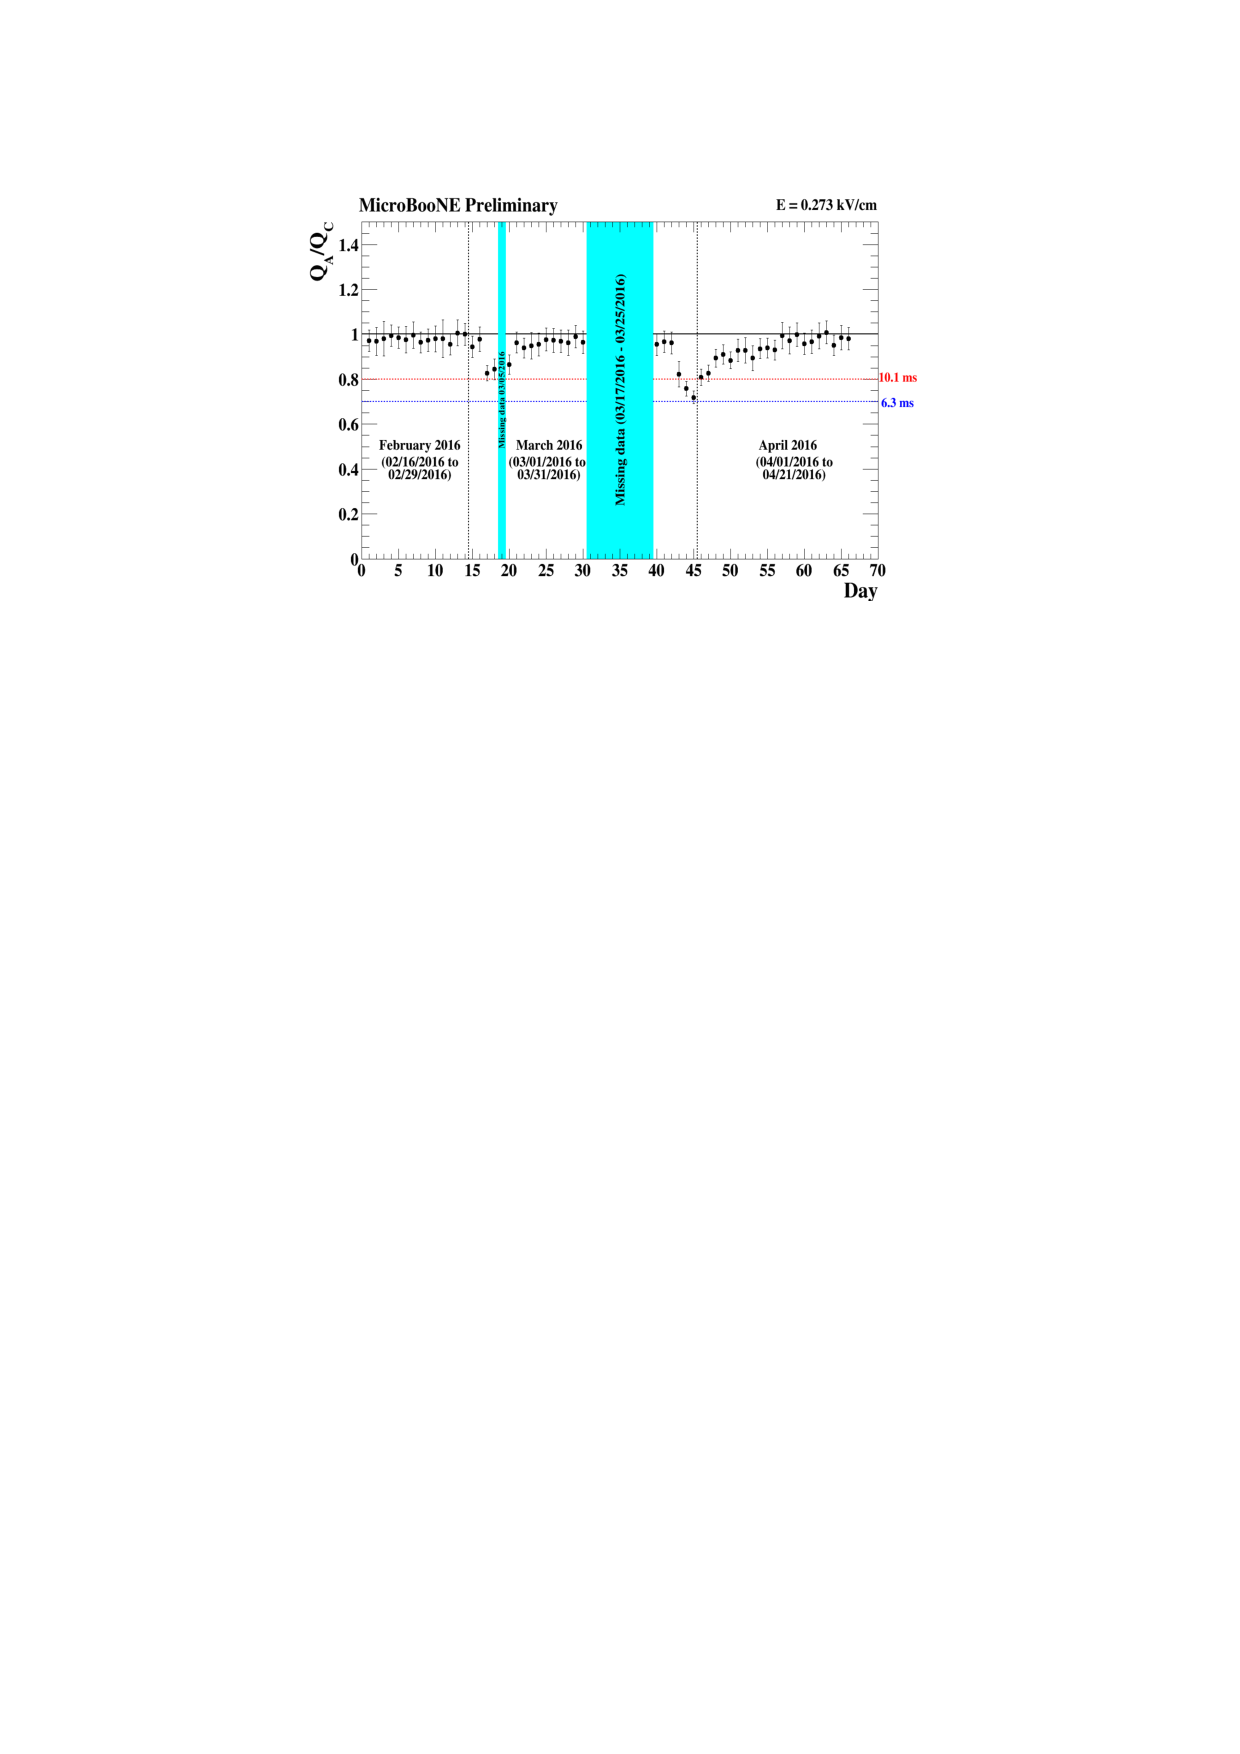
\includegraphics[width=\linewidth]{figures/purity.pdf}
%     \caption{Purity.} 
%   \end{subfigure}
  \caption{Stacked histogram of generated events as a function of the true neutrino energy, categorized into correctly identified signal events {(\emph{passed})} and different reconstruction or identification failure modes.}
  \label{fig:ineff}
\end{figure}

\subsection{Selection results}\label{sec:numu}
The previous selection efficiency results were performed with the $\nu_{e}$ CC0$\pi$-Np + cosmic sample. We now look at the selection performances when analyzing events coming from the BNB beam Monte Carlo simulation with cosmic rays in the same readout window (BNB + cosmic sample). In this case, the selected events will contain background events coming from beam and cosmic-ray events.
We divide the selected events (signal and background) into 8 categories:
\begin{description}
\item[Beam intrinsic $\nu_{e}$ CC$0\pi$-Np:] charged-current $\nu_{e}$ neutrino interaction, at least one proton (N > 1), one electron, and no other visible particles above detection threshold. This category represents the signal of our analysis.
\item[Beam intrinsic $\nu_{e}$ CC:] charged-current $\nu_{e}$ neutrino interaction that is not $\nu_{e}$ CC$0\pi$-Np or where the electron or protons were below the detection threshold defined above.
\item[Beam intrinsic $\nu_{\mu}$:] charged-current $\nu_{\mu}$ neutrino interaction.
\item[Beam intrinsic NC:] neutral current neutrino interaction (both $\nu_{\mu}$ and $\nu_{e}$).
\item[Outside fiducial volume:] a neutrino interaction which occurs outside the fiducial volume, but with one or more final-state particles inside in the fiducial volume.
\item[Cosmic contaminated] a neutrino interaction candidate with at least a cosmogenic track or shower, attached to a correctly reconstructed neutrino candidate.
\item[Cosmic] there is a neutrino interaction in the event, but we select a cosmic-ray interaction happening during the same readout window as the neutrino candidate.
\item[Data off-beam] {event with no neutrino interaction, but where a cosmic-ray interaction in time-coincidence with the beam spill triggered the event, and activity was selected as a neutrino candidate.}

\end{description}


Table \ref{tab:result} shows a summary of the selection algorithm results, with the corresponding number of events for each category.
%The numbers correspond to an exposure of the MicroBooNE detector of \num{4.34e19} protons on target (POT). This is equivalent to the amount of data analyzed here, which is a subset of the data collected from February to April 2016.

\begin{table}[htbp]
   \centering
   \begin{tabular}{llrrrrr}
     \toprule
     Category & \phantom{a} & Generated & \phantom{a} & Selected & \phantom{a} & Efficiency \\
     \midrule

     \textbf{$\nu_{e}$ CC0$\pi$-Np (signal)}  & & $32.077\pm0.006$    & & $14.531\pm0.004$  & & $(45.3\pm0.5)$~\%\\
     $\nu_{e}$ CC                             & & $39.473\pm0.006$    & & $15.789\pm0.004$  & & $(40.5\pm0.5)$~\%\\
     Beam intrinsic $\nu_{\mu}$               & & $10905.9\pm4.0$   & & $488.0\pm1.2$   & & $(4.5\pm0.2)$~\%\\
     Beam intrinsic NC                        & & $3532.8\pm2.2$    & & $334.8\pm0.8$   & & $(9.5\pm0.2)$~\%\\
     Outside fid. vol.                        & & $36634.6\pm1.0$    & & $89.8\pm0.1$    & & $(0.2\pm0.1)$~\%\\
     Data off-beam                            & & $123070.2\pm47.0$ & & $1583.0\pm4.3$  & & $(1.3\pm0.1)$~\%\\
     Cosmic contaminated                      & & $14706.4\pm6.2$   & & $376.1\pm0.3$   & & $(2.6\pm0.1)$~\%\\ 
     Cosmic                                   & & $51356.1\pm15.0$  & & $489.4\pm0.3$   & & $(1.0\pm0.1)$~\%\\

     \bottomrule
   \end{tabular}
   \caption{Summary of the selection results, showing the contribution of each event category, for a MicroBooNE exposure of \num{4.34e19} POT. Uncertainties are statistical only. {For the \emph{Cosmic contaminated} category the number of generated events correspond to the number of neutrino interactions inside the cryostat. For the \emph{Cosmic} category, it corresponds to the total number of simulated neutrino interactions, bot inside and outside the cryostat.}}\label{tab:result}
\end{table}


Figure \ref{fig:spectrum} shows the reconstructed energy spectrum of the selected events. The reconstructed energy has been measured with the procedure described in Section \ref{sec:energyreco}. The evaluation of the systematic uncertainties, represented by the shaded bars, is described in Section \ref{sec:systematics}. Both the $\chi^2$ and Kolmogorov-Sminorv tests give a probability of 1.00 (rounded up at the second decimal digit)  of the null hypothesis, which is the data distribution being compatible with the Monte Carlo simulation.
%This plot shows that our selection procedure has similar performances in data and Monte Carlo and that there is no evident bias in the energy reconstruction. 

\begin{figure}[htbp]
\centering
  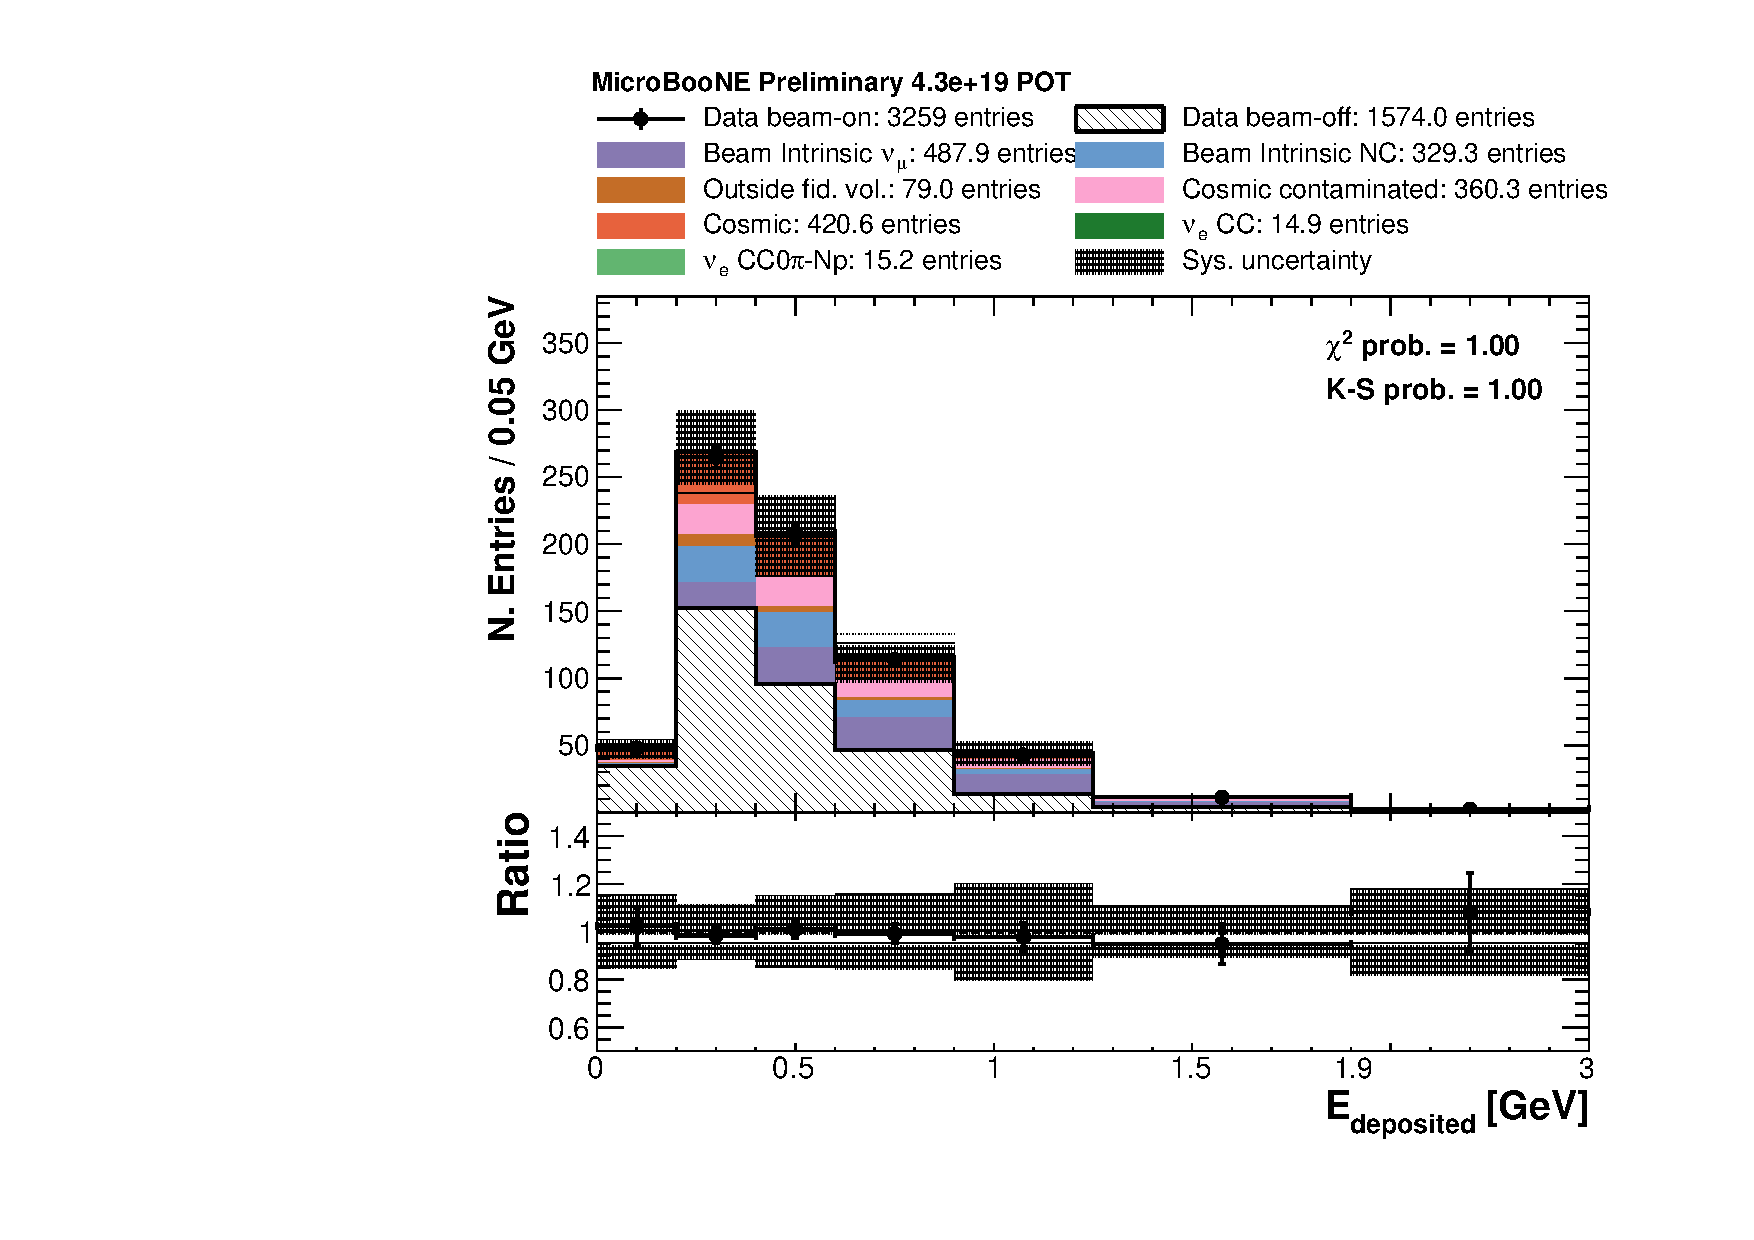
\includegraphics[width=0.65\linewidth]{figures/h_fixed_energy.pdf}
  \caption{Reconstructed energy spectrum after the event selection algorithm and the veto of the events selected by the CC $\nu_{\mu}$ module. The histograms of the event categories are stacked.}
  \label{fig:spectrum}
\end{figure}

The agreement between data and simulation is also verified in the angular distributions of the reconstructed showers objects, shown in Figure \ref{fig:thetaphi}. As expected, the neutrino distributions are mostly constant as a function of the azimuthal angle $\phi$ and peaked at low inclination angle $\theta$ values, since the interactions are mostly forward going. The inclination angle $\theta$ distribution agrees within the uncertainties both for shape and normalization. The azimuthal angle $\phi$ distribution shows a slight disagreement around $\phi = 0^{\circ}$ and $\phi = \pm180^{\circ}$. {This is caused by an imprecise signal simulation that predominantly affects tracks moving exactly towards or away from the anode \cite{signal1, signal2}. This effect is taken into account in the Dynamic Induced Charge sample (Section \ref{sec:systematics}). Figure \ref{fig:thetaphi_pdg} shows the angular distributions classified according to the primary particle that generated the shower. In this case, the data points correspond to the statistical subtraction of the beam-on and beam-off entries.}

\begin{figure}[htbp]
\centering
  \begin{subfigure}{0.49\textwidth}
    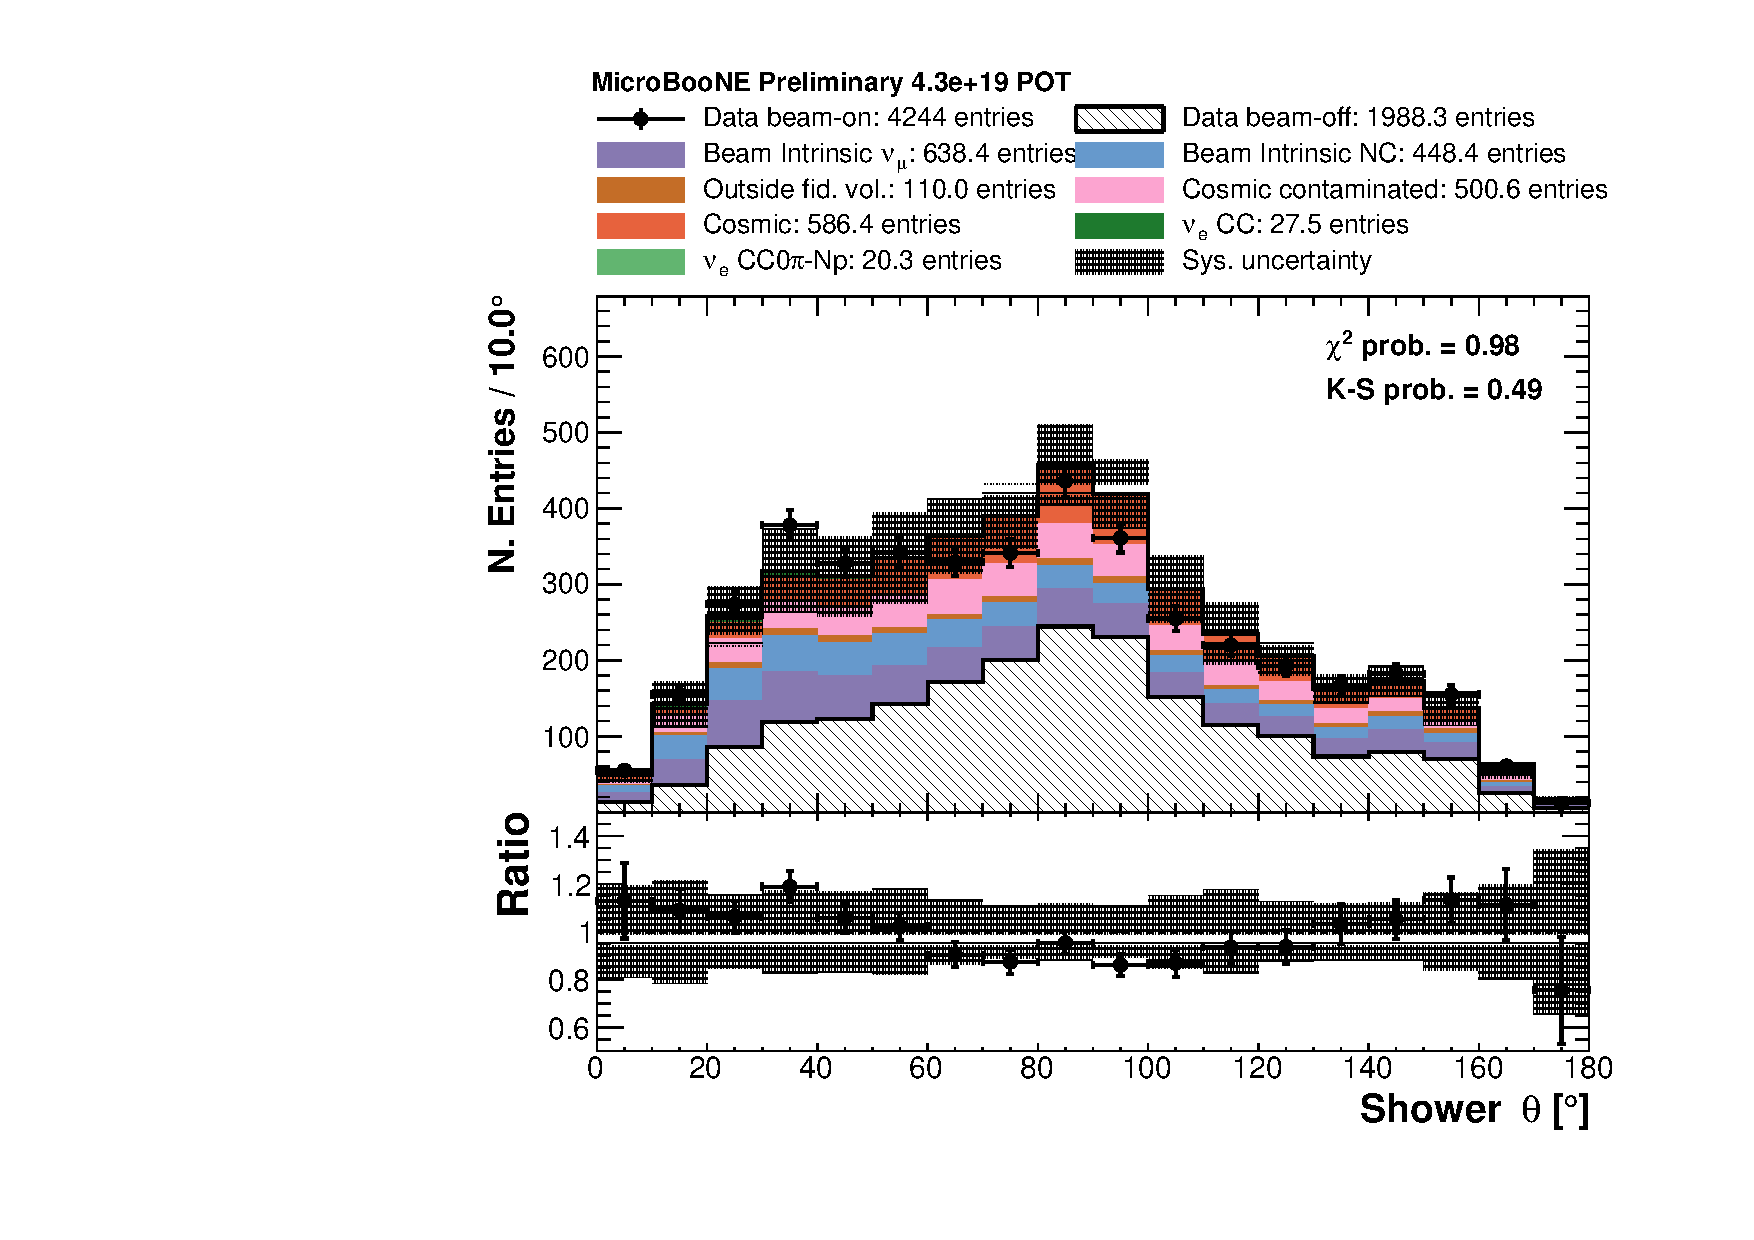
\includegraphics[width=\linewidth]{figures/h_shower_theta.pdf}
    \caption{Inclination angle $\theta$.} 
  \end{subfigure}
    \begin{subfigure}{0.49\textwidth}
    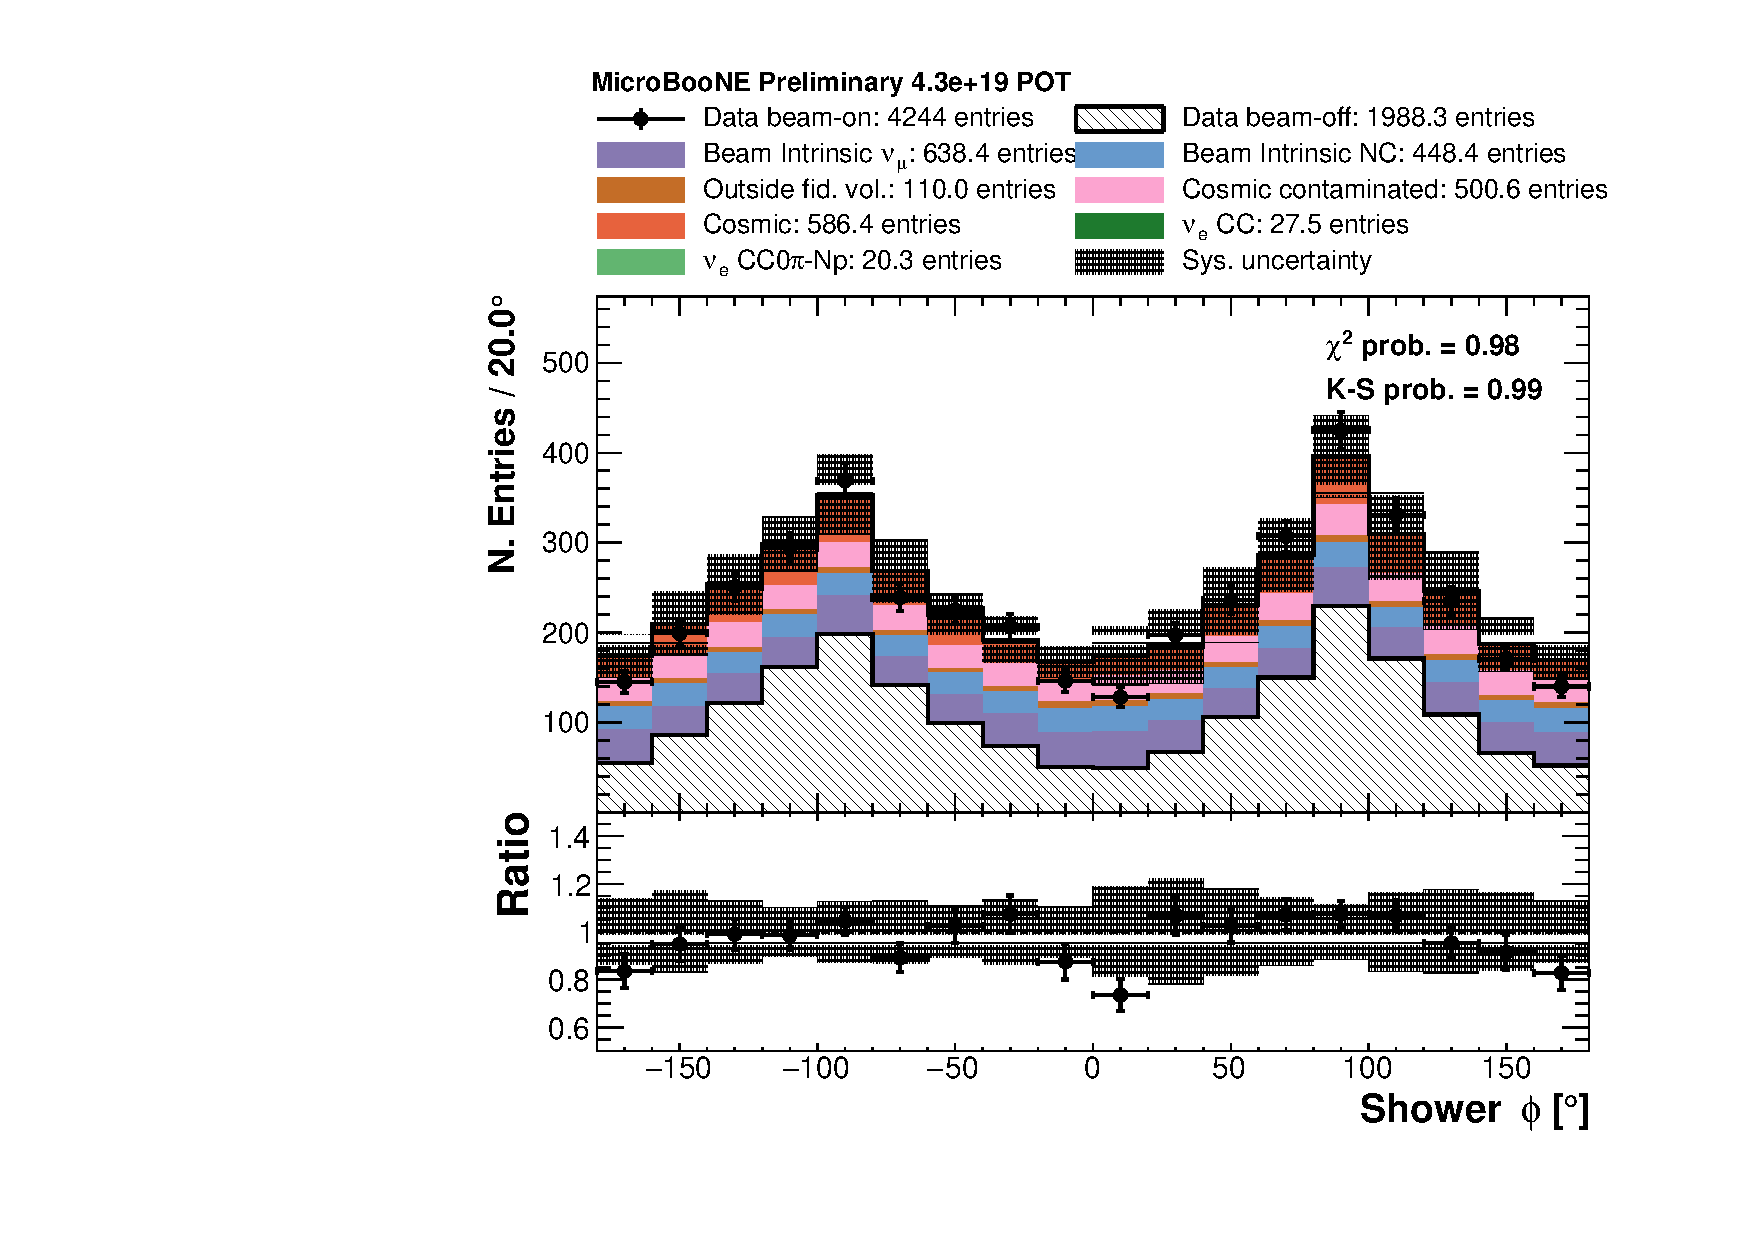
\includegraphics[width=\linewidth]{figures/h_shower_phi.pdf}
    \caption{Azimuthal angle $\phi$.} 
  \end{subfigure}
  \caption{Distributions of the inclination angle $\theta$ and the azimuthal angle $\phi$ of the reconstructed showers in the selected events for each event category.}\label{fig:thetaphi}
\end{figure}

\begin{figure}[htbp]
\centering
  \begin{subfigure}{0.49\textwidth}
    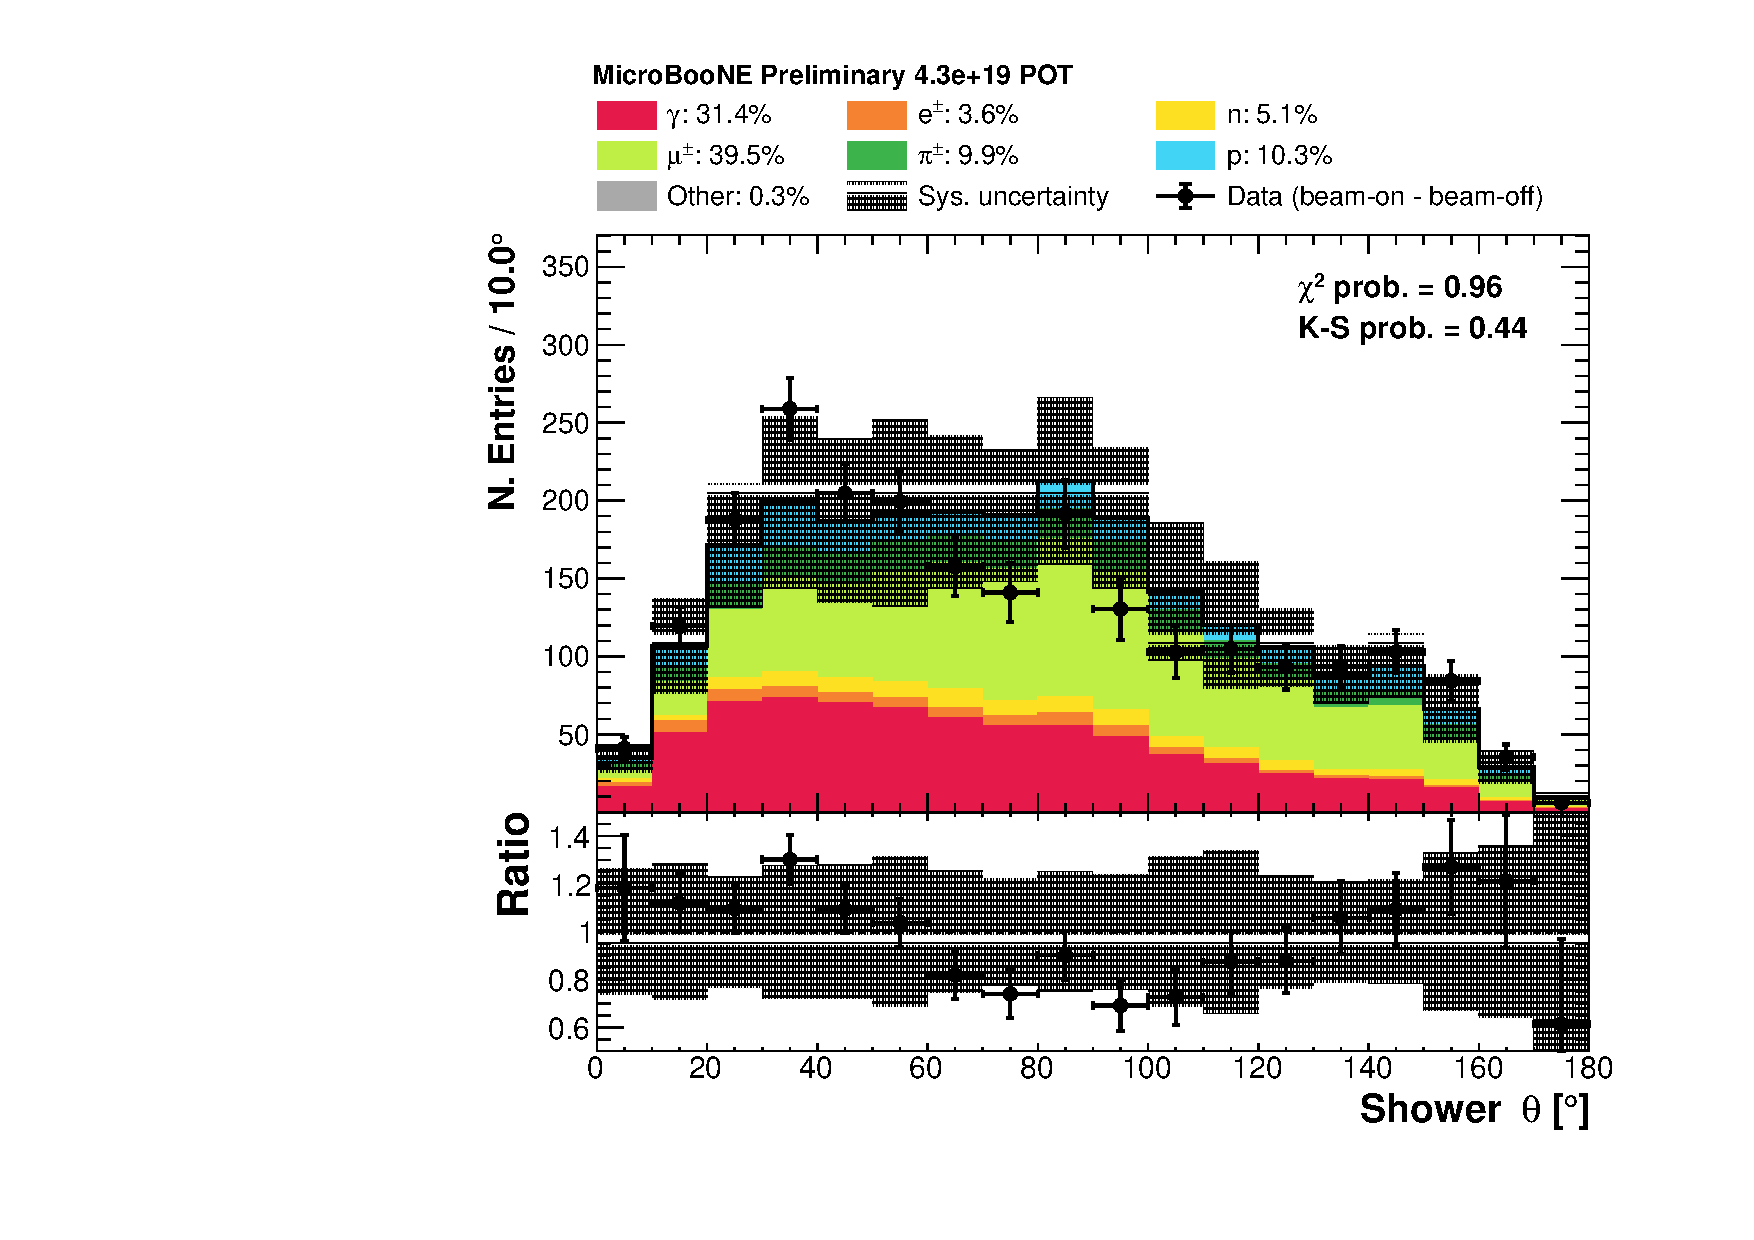
\includegraphics[width=\linewidth]{figures/h_shower_theta_pdg.pdf}
    \caption{Inclination angle $\theta$.} 
  \end{subfigure}
    \begin{subfigure}{0.49\textwidth}
    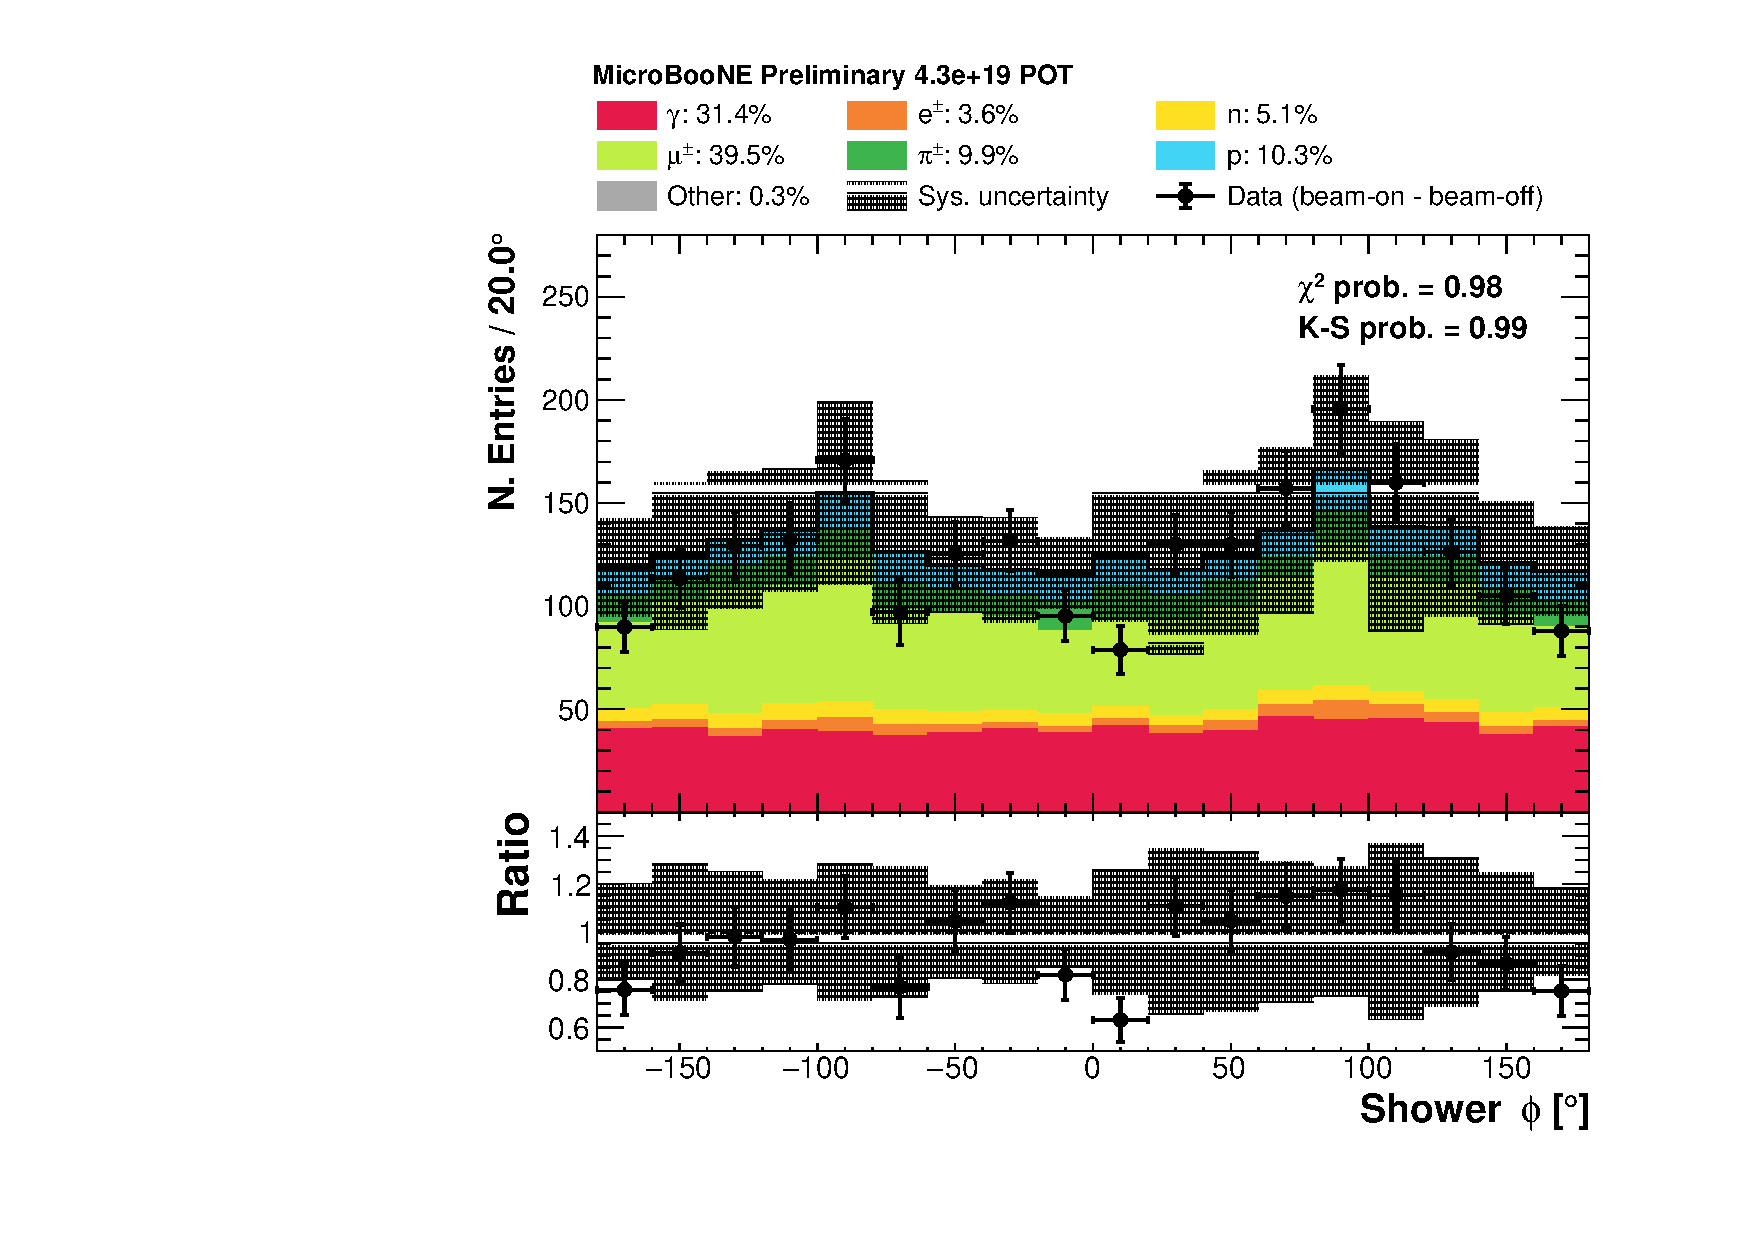
\includegraphics[width=\linewidth]{figures/h_shower_phi_pdg.pdf}
    \caption{Azimuthal angle $\phi$.} 
  \end{subfigure}
  \caption{{Distributions of the inclination angle $\theta$ and the azimuthal angle $\phi$ of the reconstructed showers, classified according to the primary particle that generated them.}}\label{fig:thetaphi_pdg}
\end{figure}

A small fraction of the data events were also visually inspected: Figure \ref{fig:evds} shows three event displays of data events compatible with a $\nu_{e}$ CC0$\pi$-Np interaction. 

\begin{figure}[htbp]
\centering
  \begin{subfigure}{0.45\textwidth}
  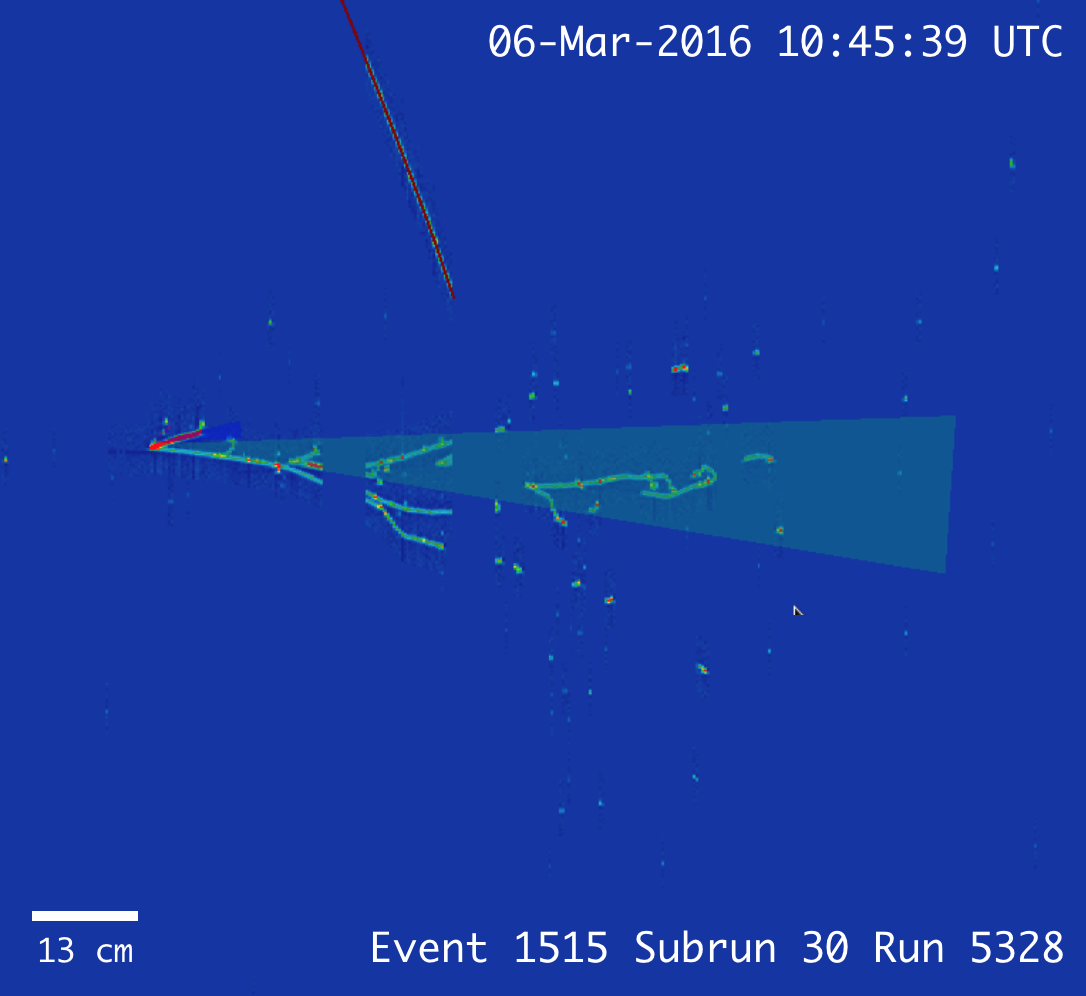
\includegraphics[width=\linewidth]{figures/data3.png}
    \caption{Event 1515, Subrun 30, Run 5328}\end{subfigure}
  \hspace{1em}\begin{subfigure}{0.45\textwidth}	
  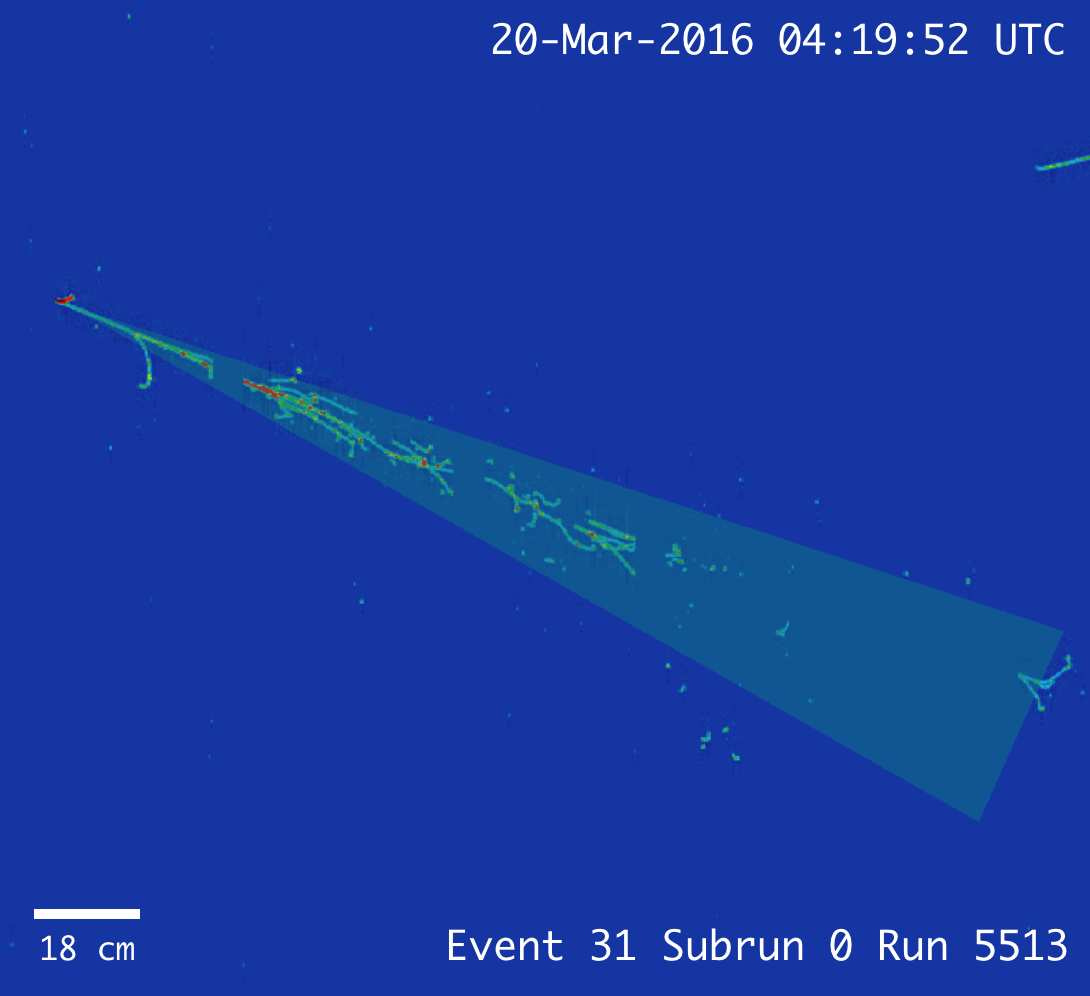
\includegraphics[width=\linewidth]{figures/data2.png}
  \caption{Event 31, Subrun 0, Run 5513}
\end{subfigure}
\vspace{1em}

  \begin{subfigure}{0.45\textwidth}	
  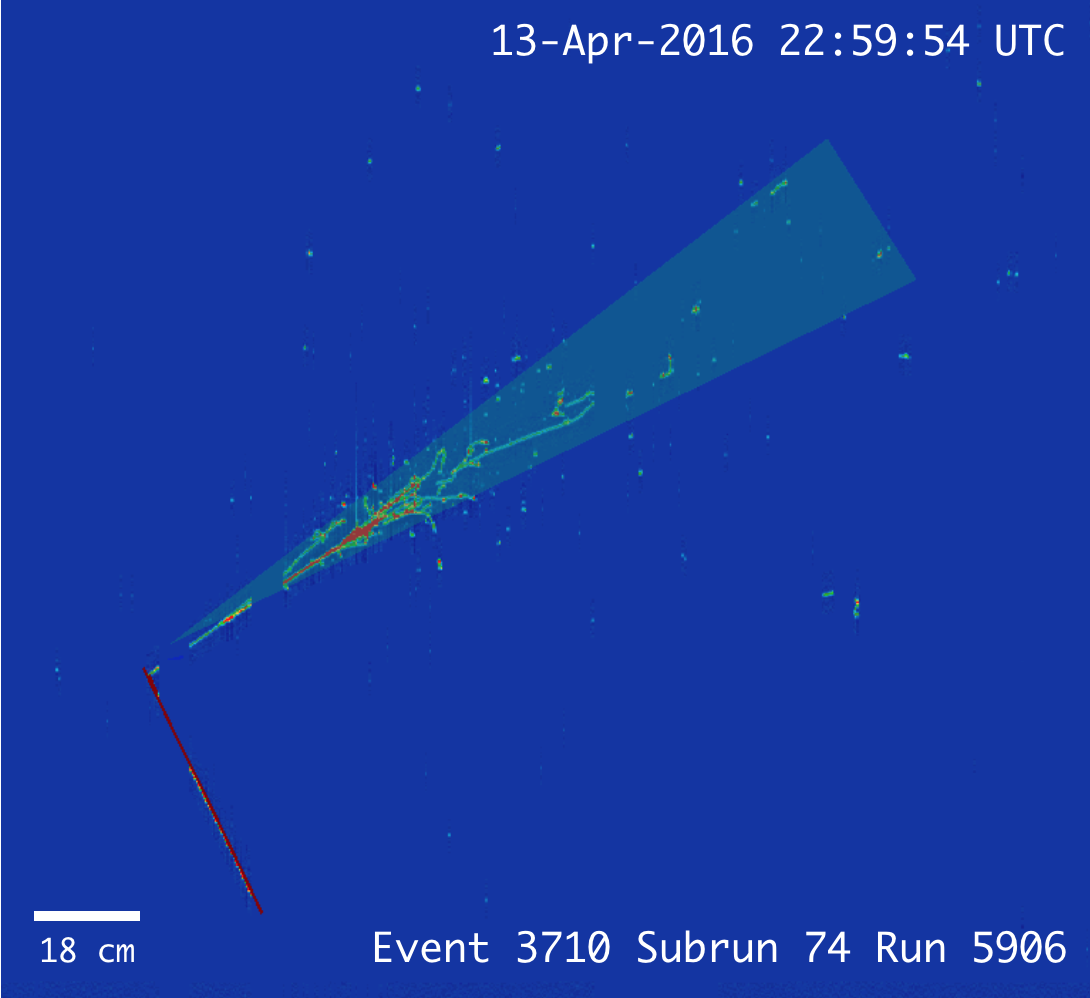
\includegraphics[width=\linewidth]{figures/data1.png}
  \caption{Event 3710, Subrun 74, Run 5906}
\end{subfigure}

  \caption{Event displays of the collection plane of three $\nu_{e}$-like data events selected by our algorithm. The gaps are caused by the presence of missing or unresponsive wires. The red lines correspond to reconstructed track-like objects and the green cones correspond to reconstructed shower-like objects. }
  \label{fig:evds}
\end{figure}



\subsection{Background Rejection}\label{sec:bkg}
In this section we will describe the cuts we could apply to our selected events, in order to isolate the $\nu_{e}$ CC$0\pi$-Np event candidates. The cuts have been chosen to (1) reduce the background, and (2) ensure that the selected events are well reconstructed. The values of each cut have been chosen manually to maximize the purity while retaining a sufficient efficiency. %It would have been possible, in theory, to calculate an optimal set of cuts, maximized by the significance of the $\nu_{e}$ CC0$\pi$-Np events. However, this set of cuts would not have allowed a correct validation of the final selected sample, due to the limited size of the data unblinded sample. As such, the chosen cuts increase the purity of our sample, but also retain a significant amount ($\approx 20$) of selected data events.


\subsubsection{Kinematic and calorimetric cuts analysis}

In this section we will study all the variables used to apply the kinematic and calorimetric cuts. In particular, we will show, for each variable:
\begin{itemize}
\item the area-normalised Monte Carlo distributions for the signal ($\nu_{e}$ CC0$\pi$-Np events), the cosmogenic background (cosmic, cosmic contaminated, and cosmic in-time), and the neutrino background ($\nu_{e}$ CC, beam intrinsic $\nu_{\mu}$, beam intrinsic NC, and outside fid. vol.), to show the rejection power of each cut;
\item the POT-normalised Monte Carlo and data distributions, to verify the agreement of the simulation with the collected data.
\end{itemize}

\begin{description}
\item[Number of reconstructed hits $> 50$.] A large number of cosmic-ray events may fake a neutrino candidate with a low number of hits. 
%This happens because the reconstruction framework is not always able to identify delta rays and Michel electrons as byproducts of the cosmic ray. We then require at least 50 reconstructed hits in order to reduce this background. 
The area-normalised distributions in Figure \ref{fig:nhits_integral} show that a large fraction of the cosmogenic backgrounds has a very low number of reconstructed hits in the collection plane, while the signal and the neutrino components have a much broader distribution. Figure \ref{fig:nhits_pot} shows a good data/Monte Carlo agreement for this variable.

\item[{Fraction of shower hits $> 0.5$.}] {Cosmic-ray and CC $\nu_{\mu}$ events faking a $\nu_{e}$ CC0$\pi$-Np candidate will have in general a long muon track and a small Michel electron at the end. In these cases, the hits associated to the reconstructed showers will represent a small fraction of the total number of hits, as shown in Figure \ref{fig:ratio_norm}. Signal events, on the contrary, have a large fraction of hits associated to shower objects. Figure \ref{fig:ratio_pot} shows the agreement between data and Monte Carlo for this quantity.}



\item[Most energetic shower $1~\mathrm{MeV/cm} < dE/dx <3.2~\mathrm{MeV/cm}$.] The rate of energy loss per length ($dE/dx$) for electromagnetic showers is measured with a procedure analogous to the one described in \cite{argoneut}. All the hits of the collection plane within a rectangle of 4~cm along the direction of the shower and 1~cm perpendicular to the shower are collected. 
The $dQ/dx$ for each hit is measured dividing the collected charge ($dQ$) by the pitch ($dx$) between each hit and the next one along the shower direction. The pitch corresponds to the distance in the TPC that a particle travels between its two projections  on adjacent wires, which is \emph{at least} the wire spacing (3~mm for MicroBooNE \cite{detector}). 
The $dE/dx$ is calculated from the $dQ/dx$ by using the calibration factor measured in Section \ref{sec:showerenergy}, eq. \eqref{eq:calib}.
Since the distribution of the $dE/dx$ hit values has an asymmetric tail due to the Landau nature of the process, we assign to the shower the median (and not the mean) of the $dE/dx$ hit distribution.
Figure \ref{fig:dedx_norm} shows that the signal distribution is peaked around 2 MeV/cm, as expected. The peak around 0~MeV/cm is caused by showers with a low number of associated hits, or where the shower was mostly aligned with the wires of the collection plane (having as such a high pitch value). The beam intrinsic NC component has a second peak around 4 MeV/cm, mainly caused by $\pi^0\rightarrow2\gamma$ decays. Thus we apply the cut $1~\mathrm{MeV/cm} < dE/dx <3.2~\mathrm{MeV/cm}$, around the electron peak. The POT-normalised plots (Figure \ref{fig:dedx_pot}, \ref{fig:dedx_pdg}) shows a good agreement between data and Monte Carlo.


% \item[Track distance $d_{t} < 5$~cm.] A well reconstructed event with a proton in the final state will have a reconstructed track attached to the reconstructed neutrino vertex. This conservative cut can be tightened as understanding of the spatial resolution improves. The most proton-like track, chosen using the score assigned by the proton BDT, is required to be within 5~cm of the reconstructed neutrino vertex.
% Figure \ref{fig:track_norm} shows that the distributions of the distance between the start point of the most proton-like track and the reconstructed neutrino vertex for signal and background are very similar. The cut $d_{t} < 5$~cm, then, mainly ensures that the event is well reconstructed. 
% %The data/Monte Carlo agreement in Figure \ref{fig:track_pot} is good, except for the first bin ($0~\mathrm{cm} < d_{t} < 0.5~\mathrm{cm}$), where we have a 10\% more Monte Carlo events than data. This small discrepancy could be explained by a slightly better vertex resolution in the simulation compared to data.

\item[Shower distance $d_{s} < 5$~cm.] Liquid argon TPCs such as MicroBooNE can distinguish between photons and electrons in two ways: (1) measuring the $dE/dx$ of the start of the electromagnetic shower, and (2) measuring the gap between the interaction vertex and the start of the electromagnetic shower. In fact, photons produced in the final state of the neutrino interaction can travel several centimeters without interacting. In order to suppress events with a photon in the final state, the most energetic shower starting point is required to be within 5 cm of the reconstructed neutrino vertex.
Figure \ref{fig:showerd_norm} shows the distributions of the distance between the start point of the most energetic shower and the reconstructed neutrino vertex for signal and background events. As expected, background neutrino events have a slightly larger tail than the signal events. The agreement between data and Monte Carlo shown in Figure \ref{fig:showerd_pot} {and Figure \ref{fig:showerd_pdg}} is good. Improvements currently implemented in the Pandora framework will allow for more appropriate cuts to further reduce the photon background.

\item[Track proton $\chi^2 < 80$.] It is possible to perform a $\chi^2$ test on the $dE/dx$ vs. residual range of the reconstructed track under the hypothesis of a proton stopping in the detector. Lower values of the $\chi^2$ score will correspond to proton-like tracks, while a high value will correspond to a MIP-like track. Figure \ref{fig:proton_norm} shows the distributions of the $\chi^2$ score for background and signal events. The peak at 0 for the signal events correspond to proton correctly reconstructed as tracks, while the long tail includes shower remnants classified as tracks and events with a misplaced vertex. The agreement between data and Monte Carlo shown in Figure \ref{fig:proton_pot} shows some discrepancies, especially for very low and very high $\chi^2$ scores. This quantity requires a careful simulation of the signal processing and a correct evaluation of the recombination effect. Our cut in a region with a good data/Monte Carlo agreement once the systematic uncertainties are taken into account and it is as such deemed safe.

\item[Track-shower angle $\mathrm{cos}\alpha > -0.9$]. Electrons often start producing an appreciable shower in the detector after several centimeters. As such, the reconstruction framework identifies the first part of the shower as a track-like object and the latter part of the shower as a shower-like object. 
Furthermore, high-energy cosmic rays can produce a shower in the detector, which will be mostly aligned to a cosmic muon track. In order to remove these mis-reconstructed events and reduce this kind of cosmogenic background we require $\mathrm{cos}\alpha > -0.9$, where $\alpha$ is the angle between the most energetic shower and the most proton-like track, as identified by the proton BDT.
Figure \ref{fig:angle_integral} shows that there are, in proportion, more background events for events with a high angular separation between the most proton-like track and the most energetic shower. This cut allows to reject these events while also ensuring that the signal events are well-reconstructed. In fact, signal events with $\mathrm{cos}\alpha \approx -1$ have almost always an electron shower reconstructed as a track-like object in the first part. The agreement shown in Figure \ref{fig:angle_pot} is good. Future improvements to the shower reconstruction will allow for an increased selection efficiency.


\item[Most proton-like track length $L < 80~\mathrm{cm}$]. Our signal sample will contain only protons in the final state. Protons in liquid argon have a higher stopping power than muons, which will correspond on average to shorter tracks. The track with the lowest $\chi^{2}$ proton score is required to be shorter than 80 cm. This cut helps rejecting mainly CC $\nu_{\mu}$ events with high-energy muons in the final state. 
Both neutrino and cosmic background events have on average longer reconstructed tracks than signal events, as shown in Figure \ref{fig:length_norm}. The cut $L < 80~$cm increases the signal purity without significantly decreasing the signal efficiency. The agreement between data and Monte Carlo distributions is good (Figures \ref{fig:length_pot}, \ref{fig:length_pdg}). A dedicated particle identification algorithm currently under development will replace this cut in the future.

\end{description}


\begin{figure}[htbp]
\centering
  \begin{subfigure}{0.49\textwidth}
    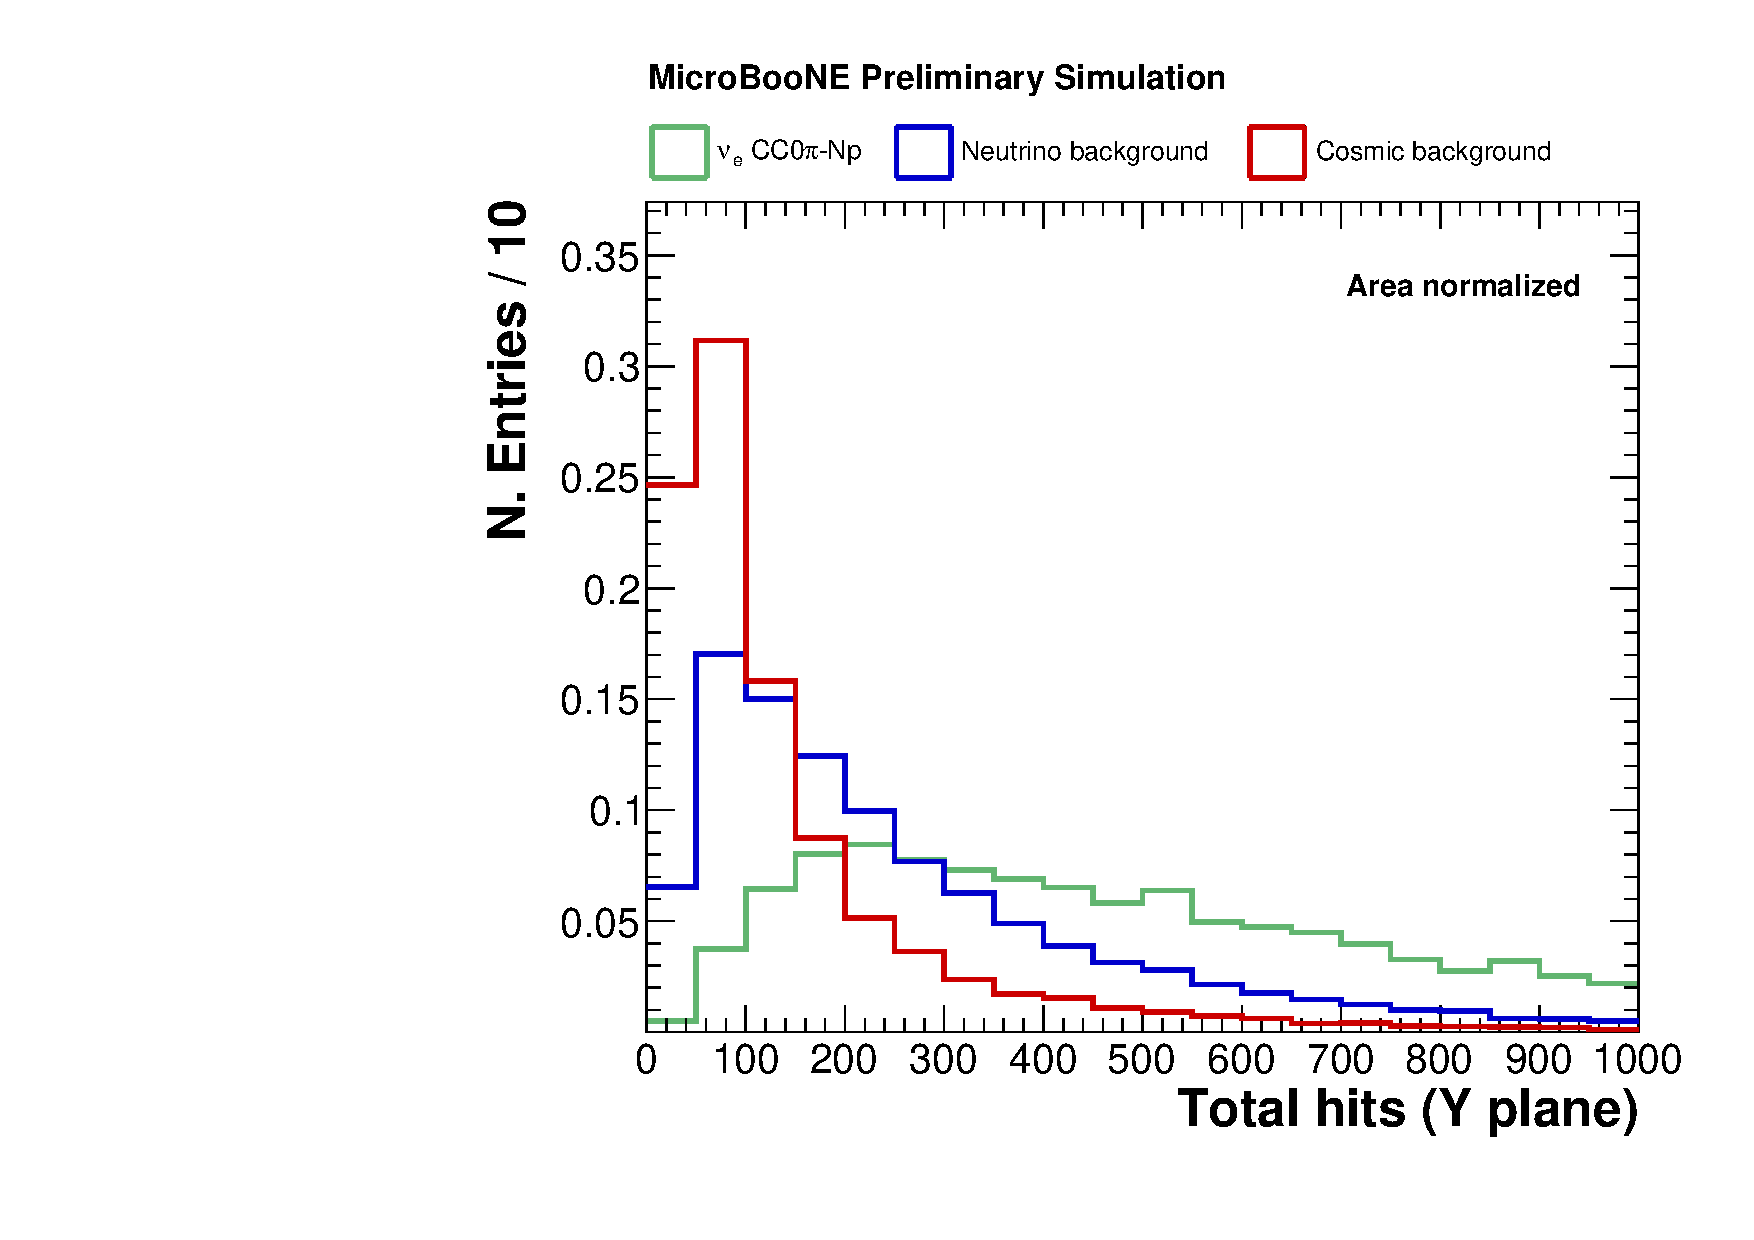
\includegraphics[width=\linewidth]{figures/h_total_hits_y_norm.pdf}
    \caption{Area normalised.} \label{fig:nhits_integral}
  \end{subfigure}
    \begin{subfigure}{0.49\textwidth}
    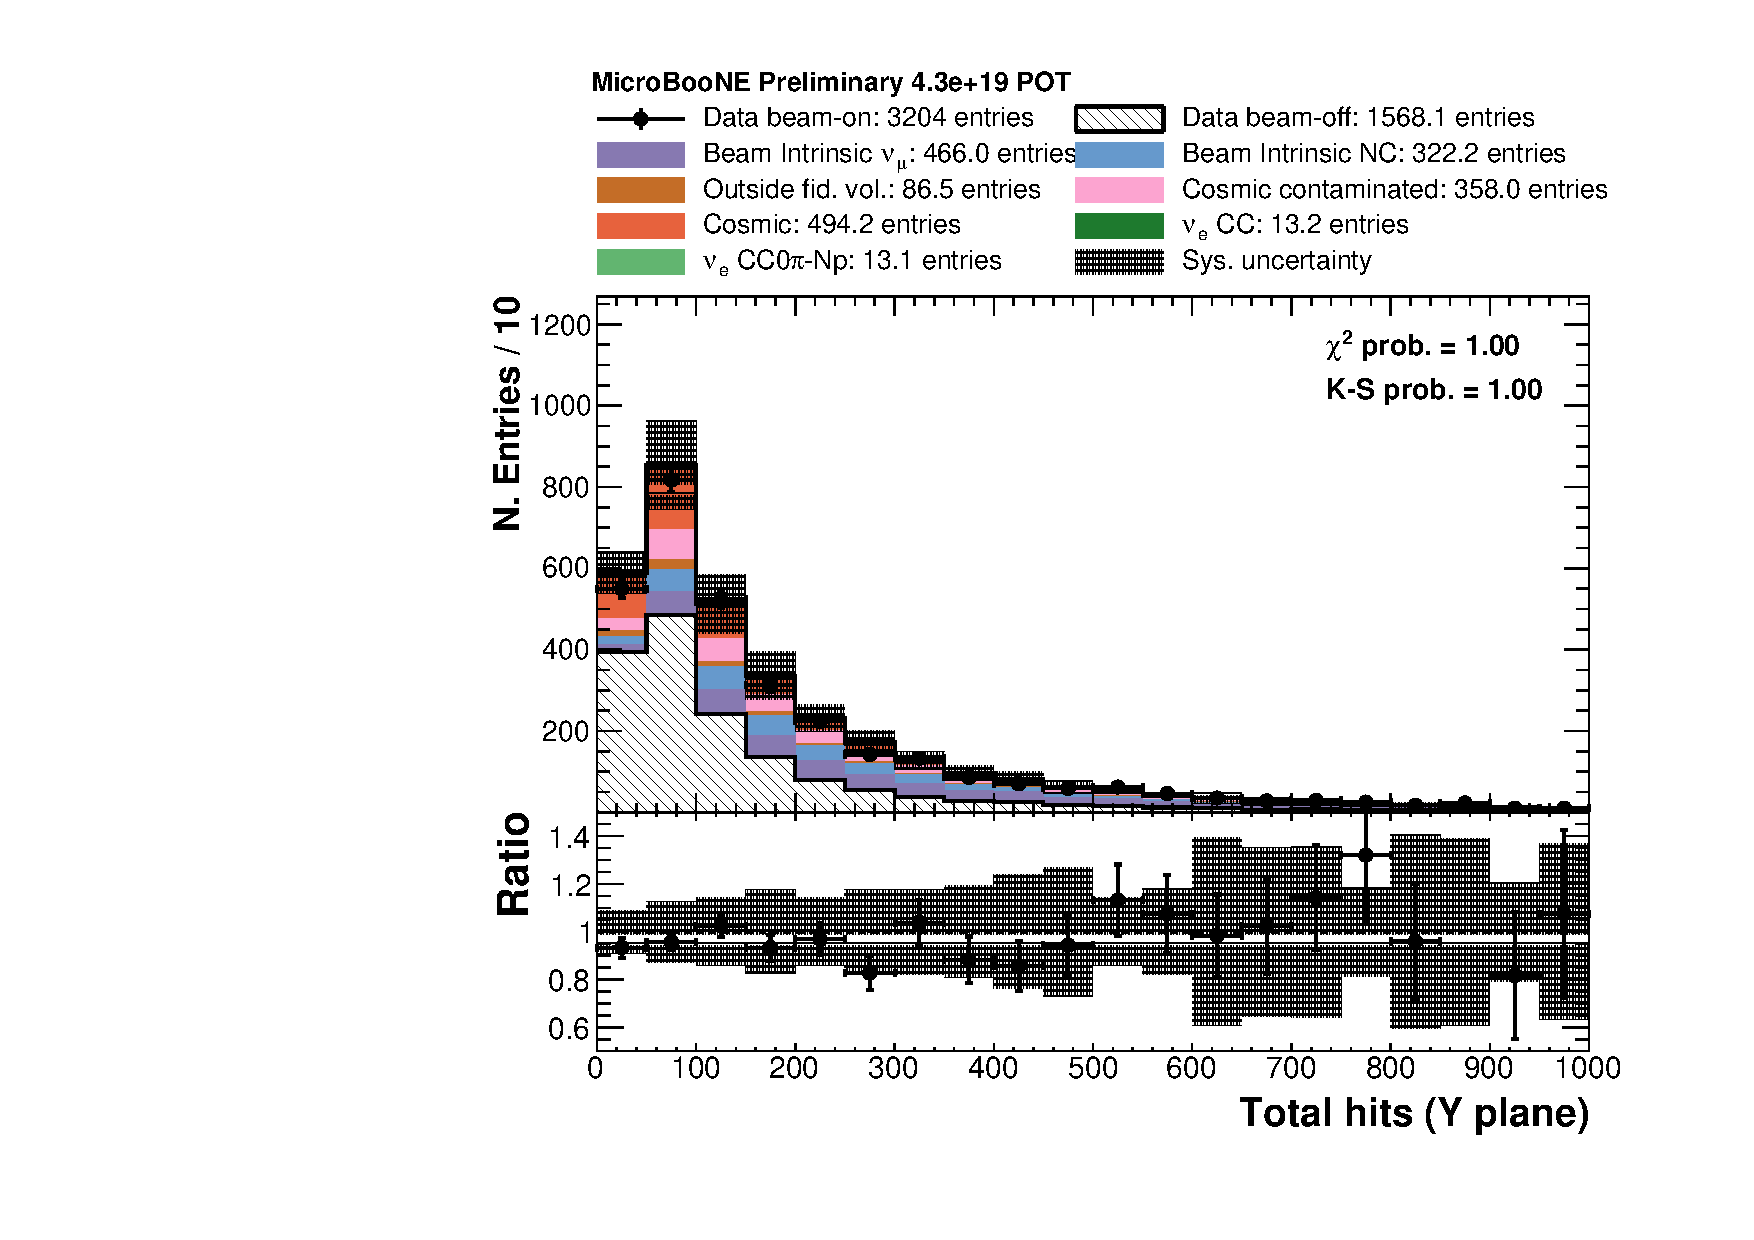
\includegraphics[width=\linewidth]{figures/h_total_hits_y.pdf}
    \caption{POT normalised.} \label{fig:nhits_pot}
  \end{subfigure}
  \caption{Area and POT normalised distributions of the number of reconstructed hits in the collection plane for all the objects in the event.}
\end{figure}

\begin{figure}[htbp]
\centering
  \begin{subfigure}{0.49\textwidth}
    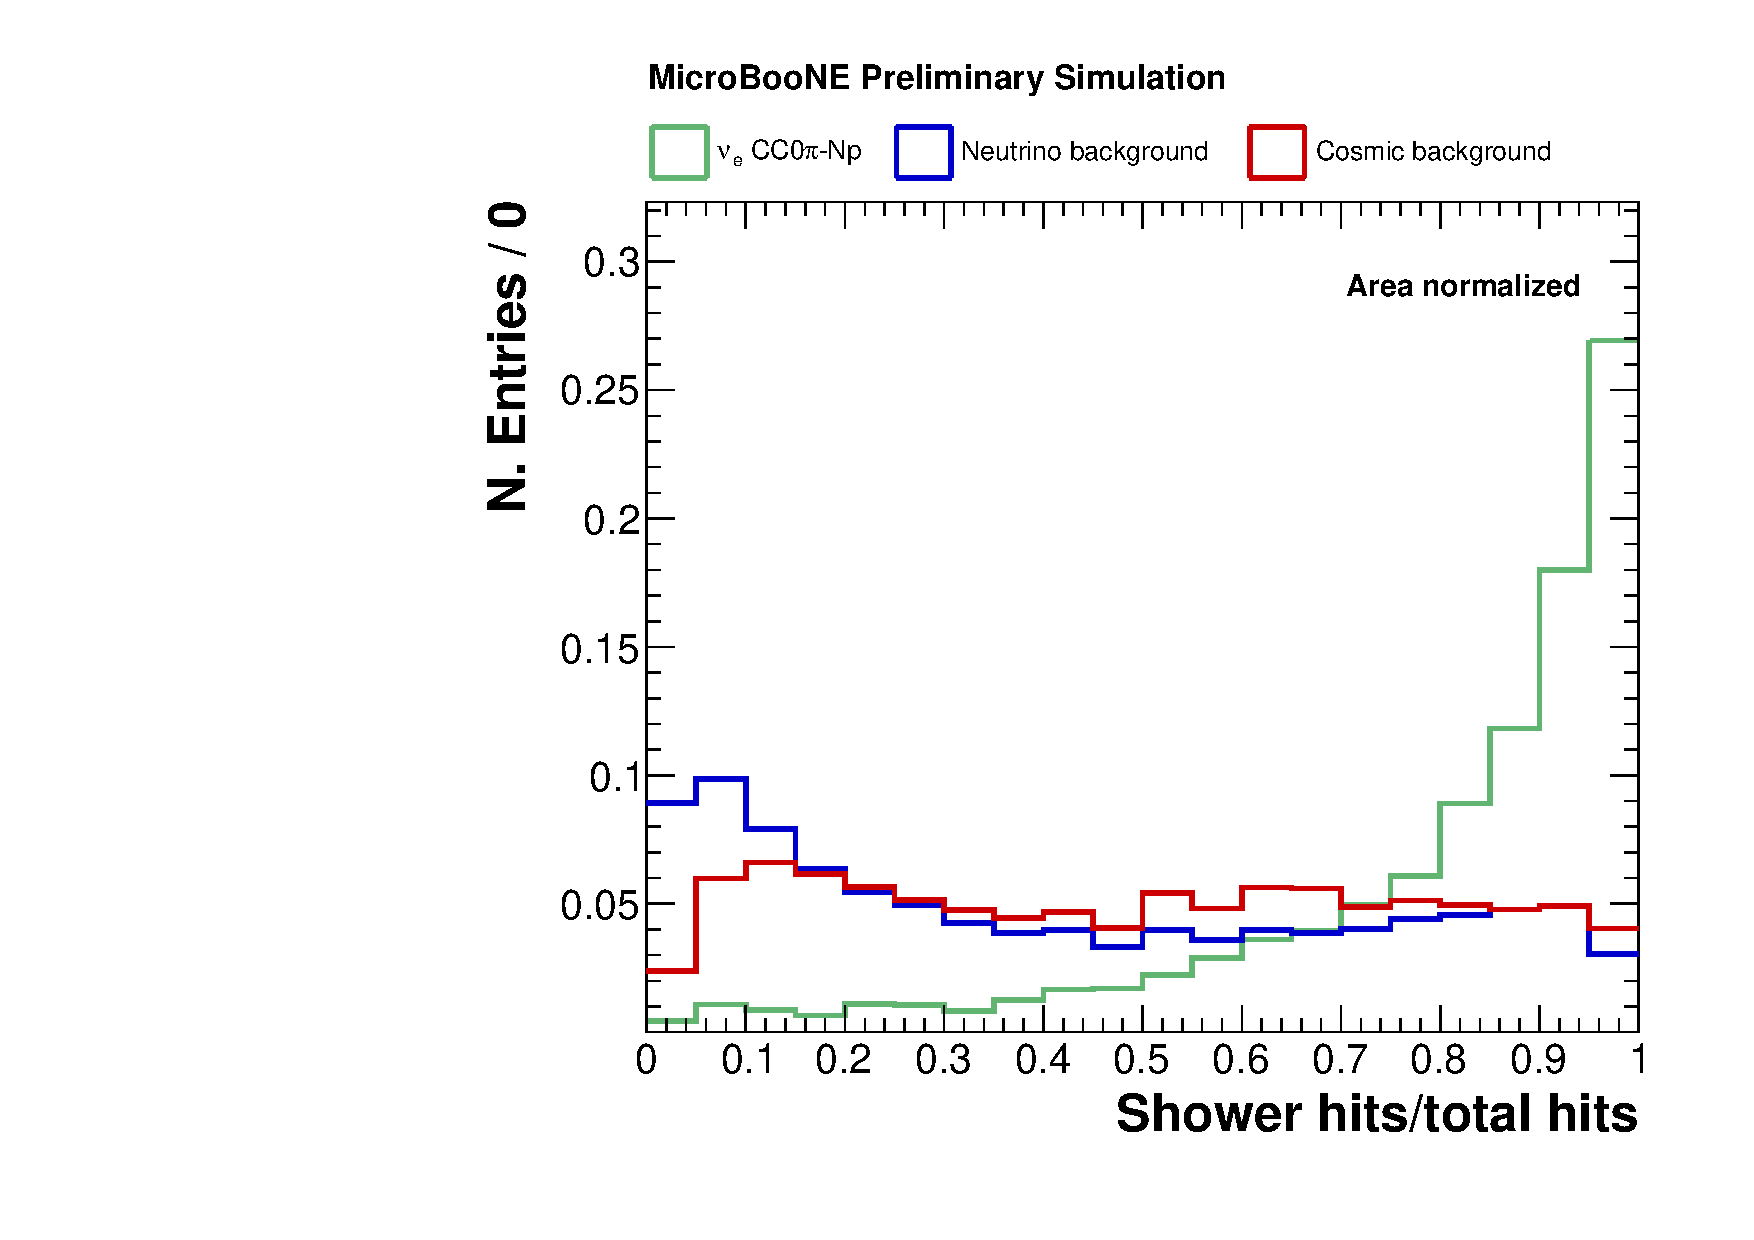
\includegraphics[width=\linewidth]{figures/h_hits_ratio_norm.pdf}
    \caption{Area normalised.} \label{fig:ratio_norm}
  \end{subfigure}
    \begin{subfigure}{0.49\textwidth}
    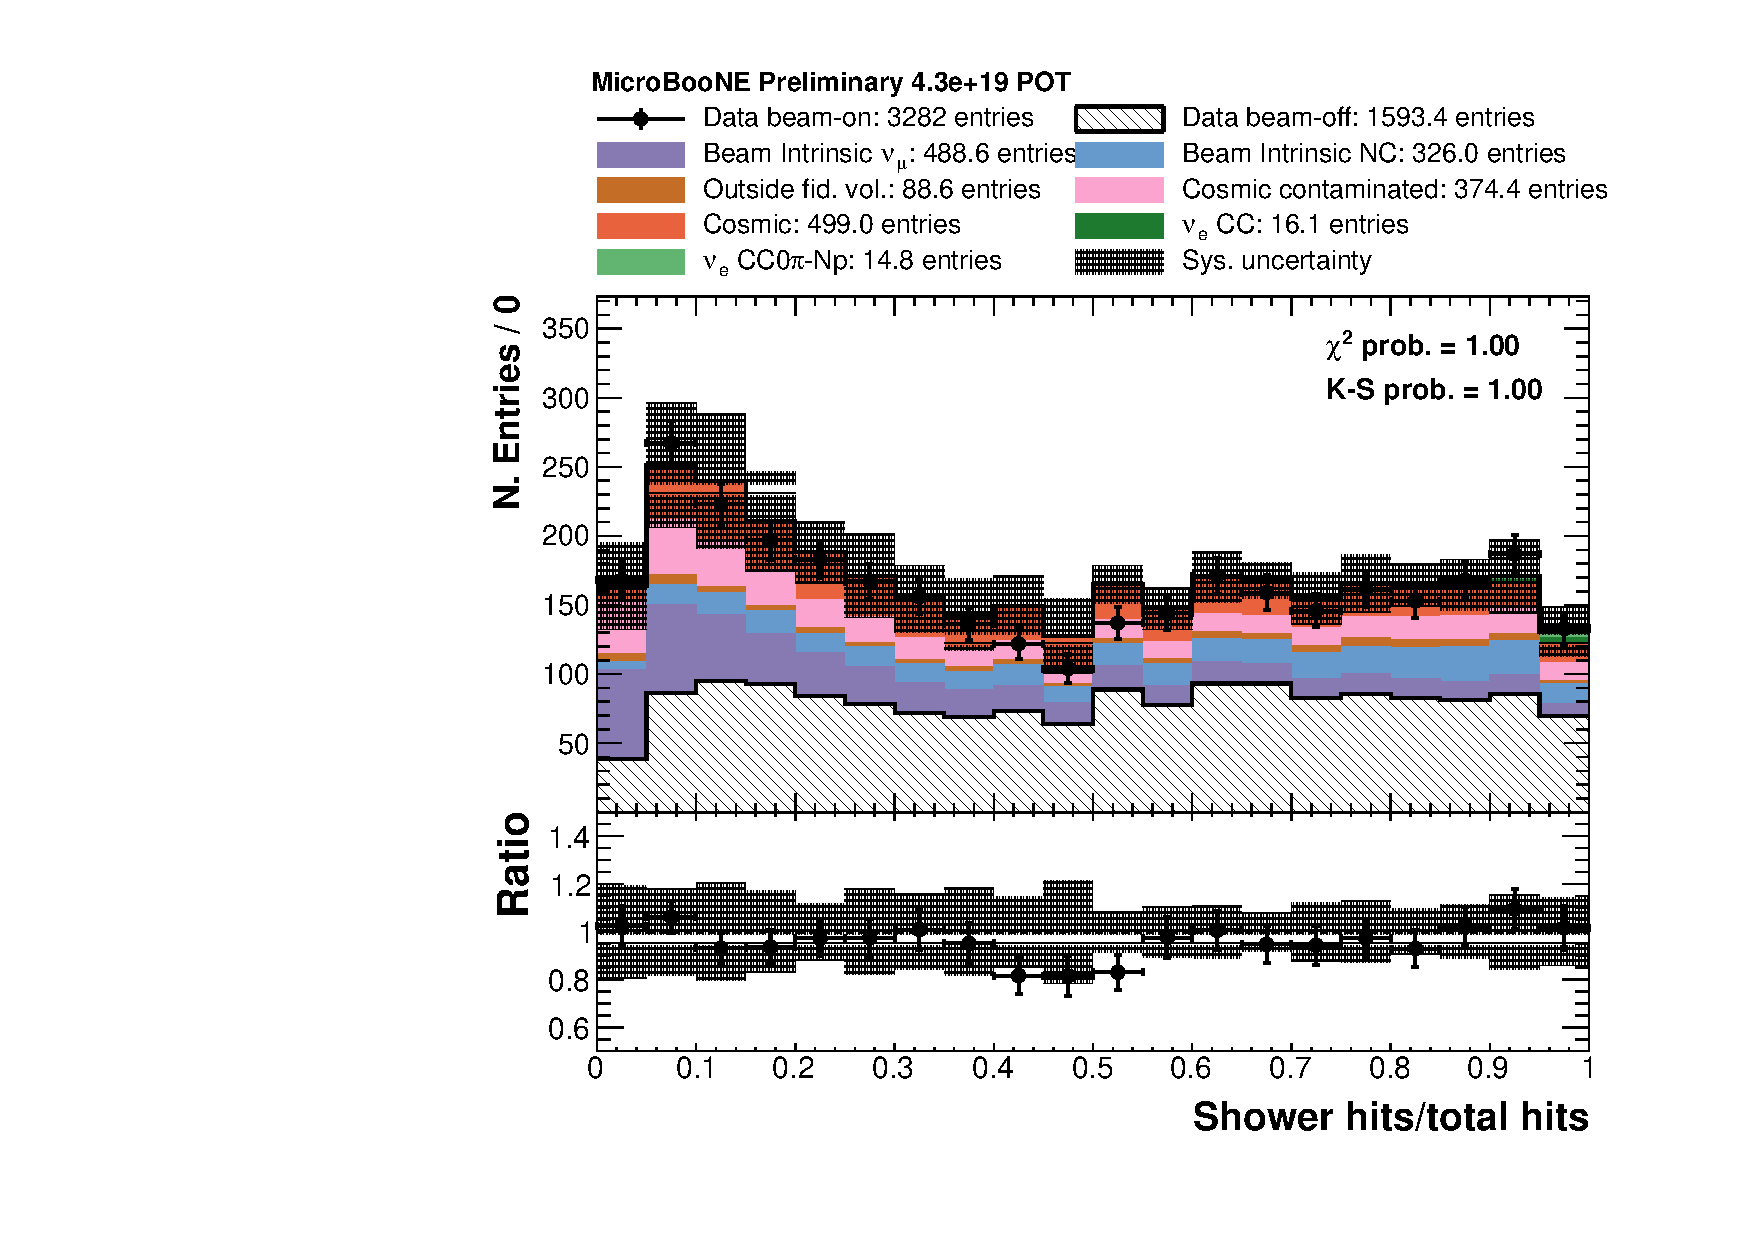
\includegraphics[width=\linewidth]{figures/h_hits_ratio.pdf}
    \caption{POT normalised.} \label{fig:ratio_pot}
  \end{subfigure}
  \caption{Area and POT normalised distributions of the ratio between the hits associated to reconstructed showers and the total number of reconstructed hits in the collection plane.}
\end{figure}

\begin{figure}[htbp]
\centering
  \begin{subfigure}{0.49\textwidth}
    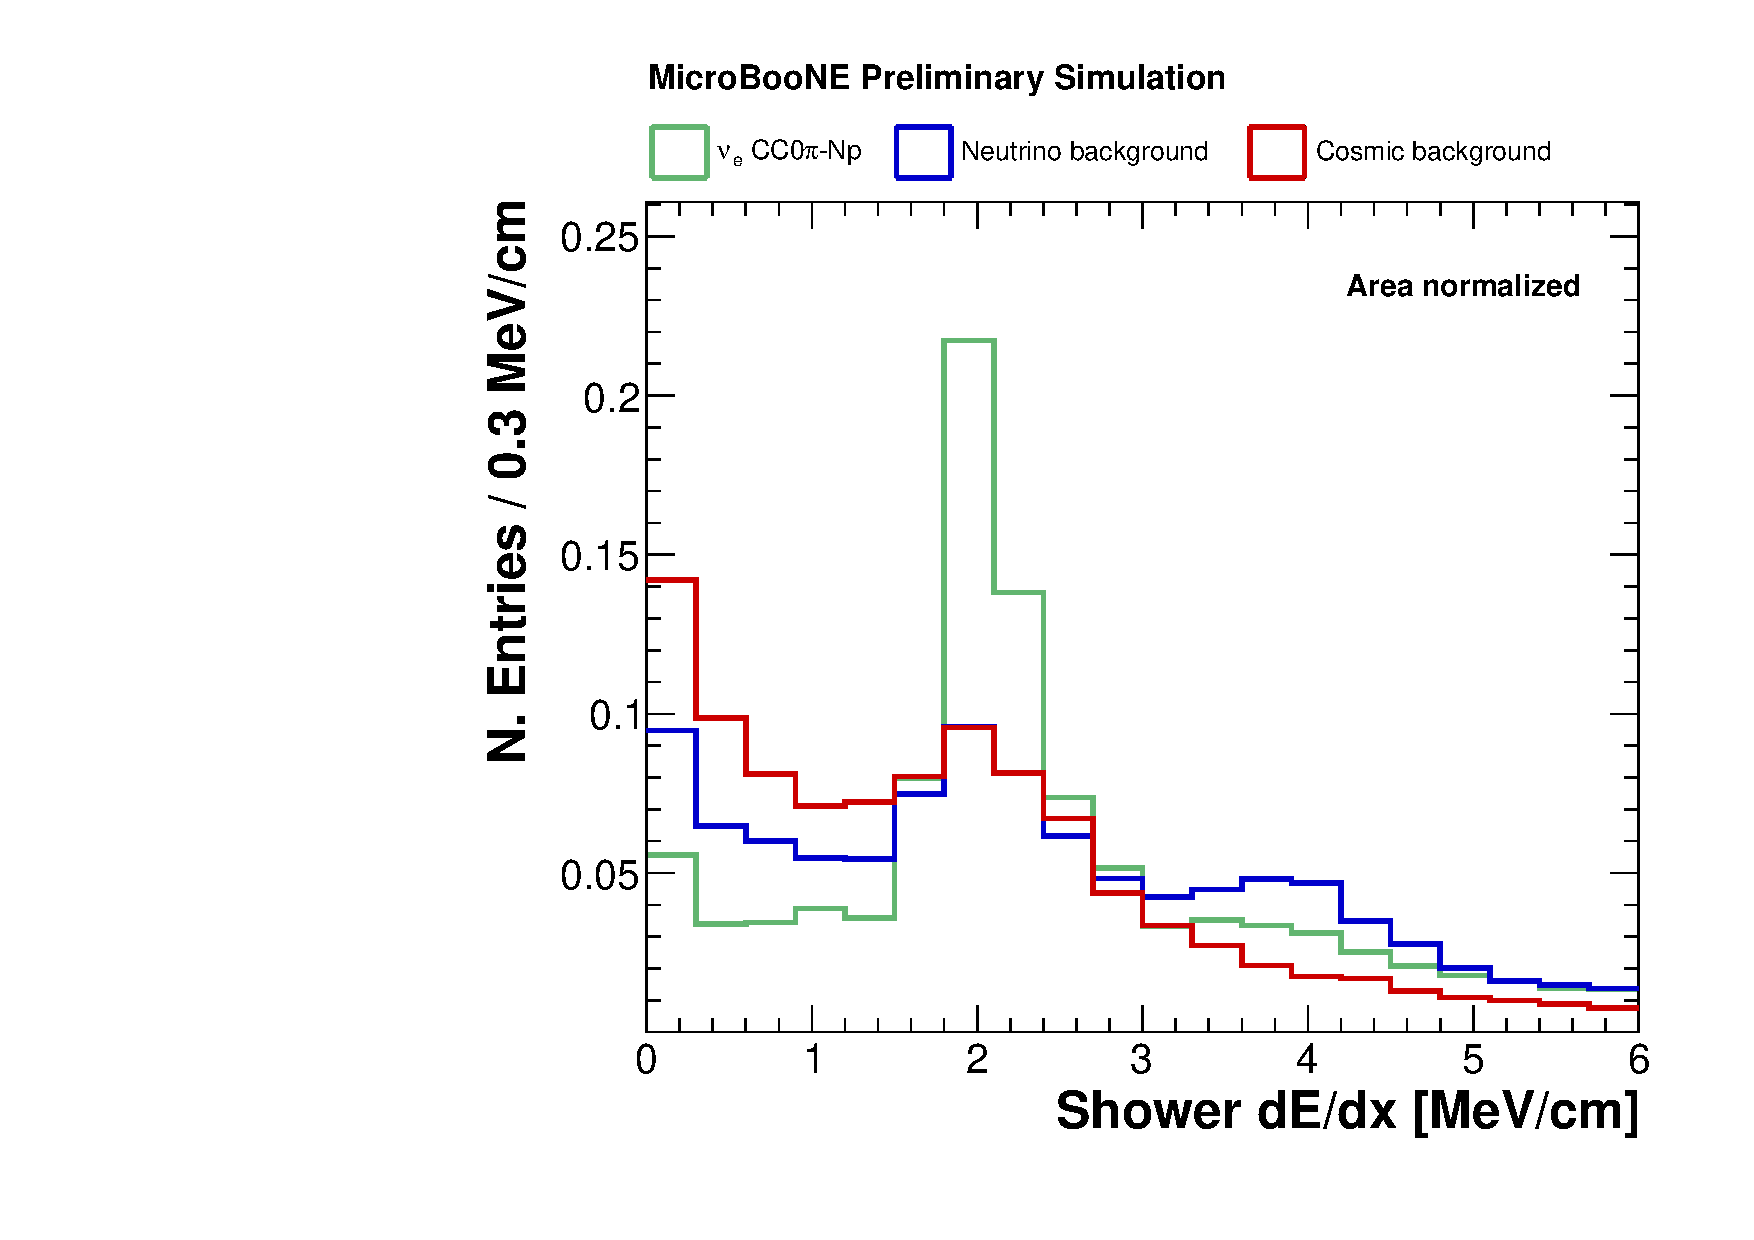
\includegraphics[width=\linewidth]{figures/h_shower_dedx_cali_norm.pdf}
    \caption{Area normalised.} \label{fig:dedx_norm}
  \end{subfigure}
    \begin{subfigure}{0.49\textwidth}
    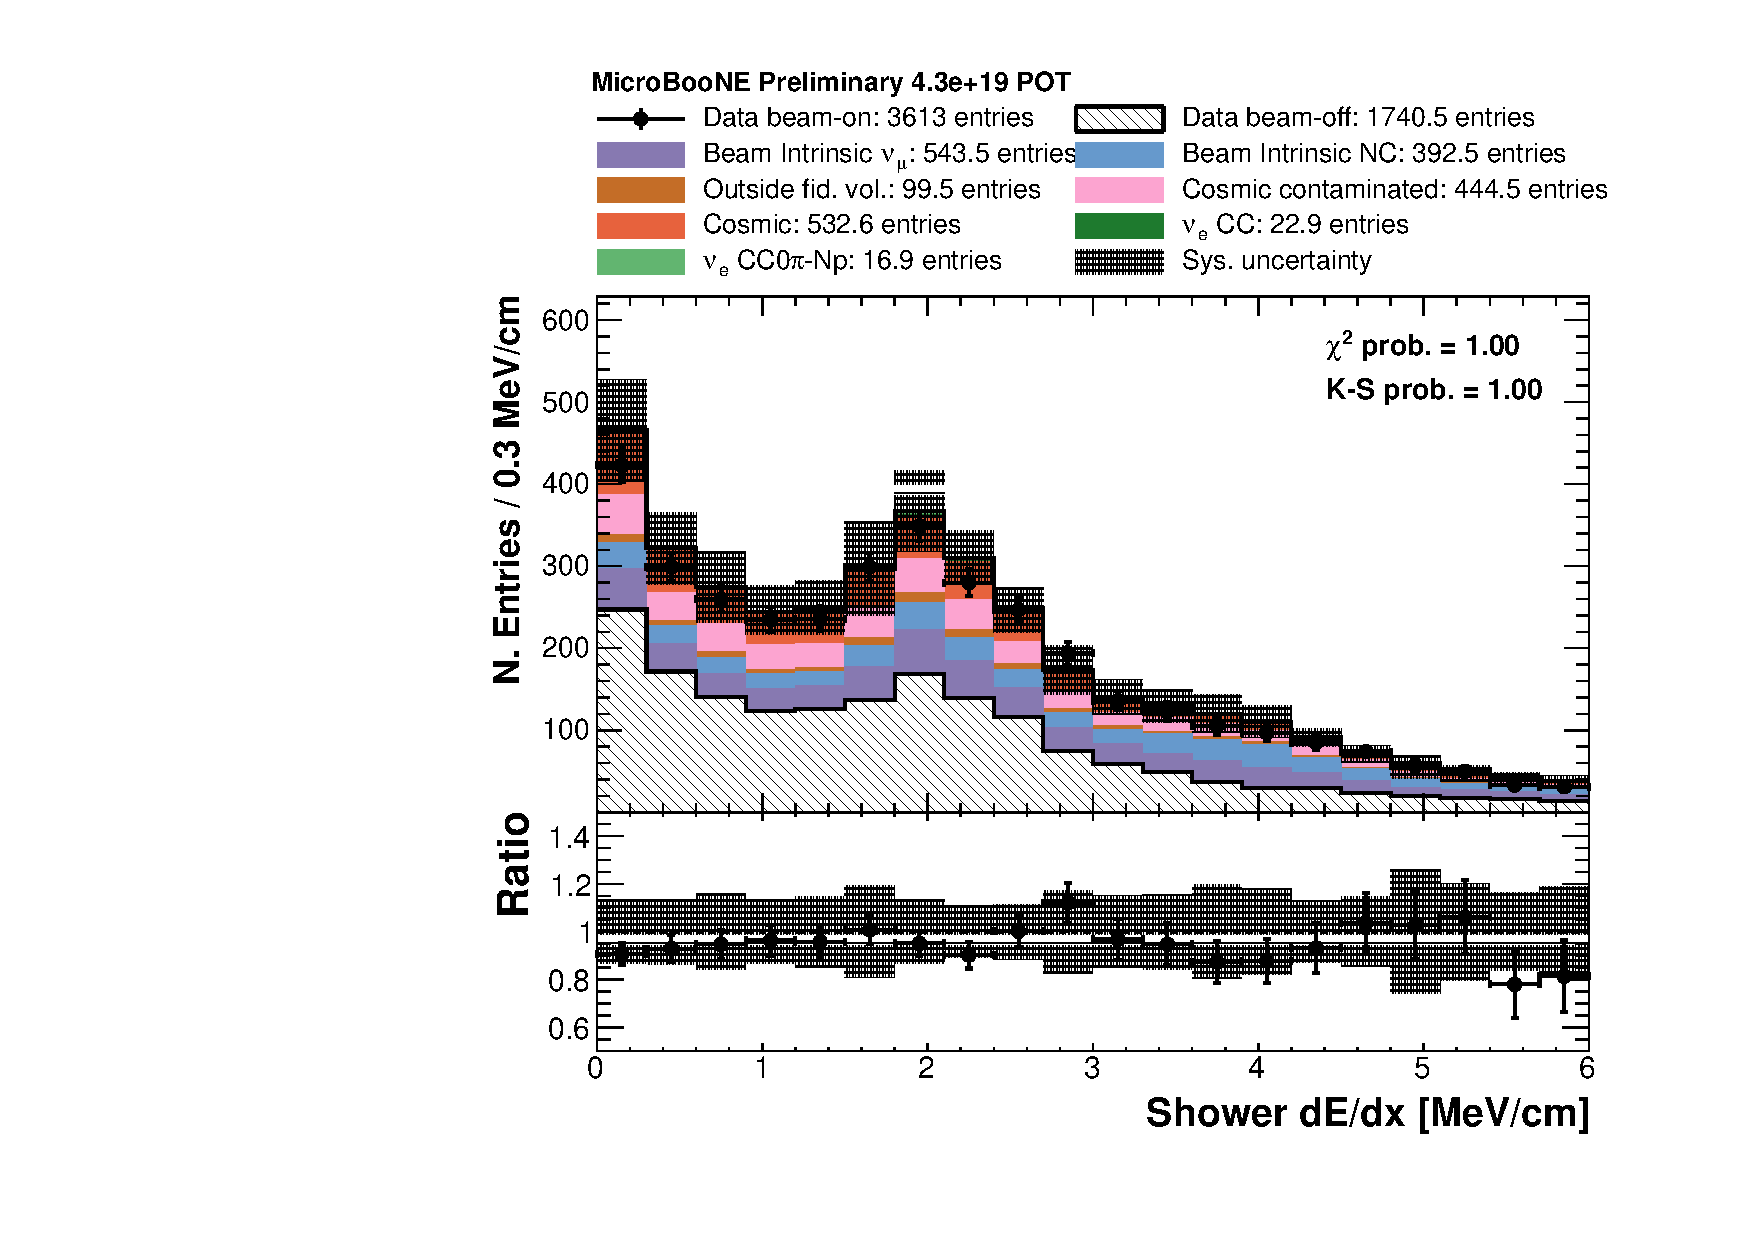
\includegraphics[width=\linewidth]{figures/h_shower_dedx_cali.pdf}
    \caption{POT normalised, event category.} \label{fig:dedx_pot}
  \end{subfigure}
  \begin{subfigure}{0.49\textwidth}
    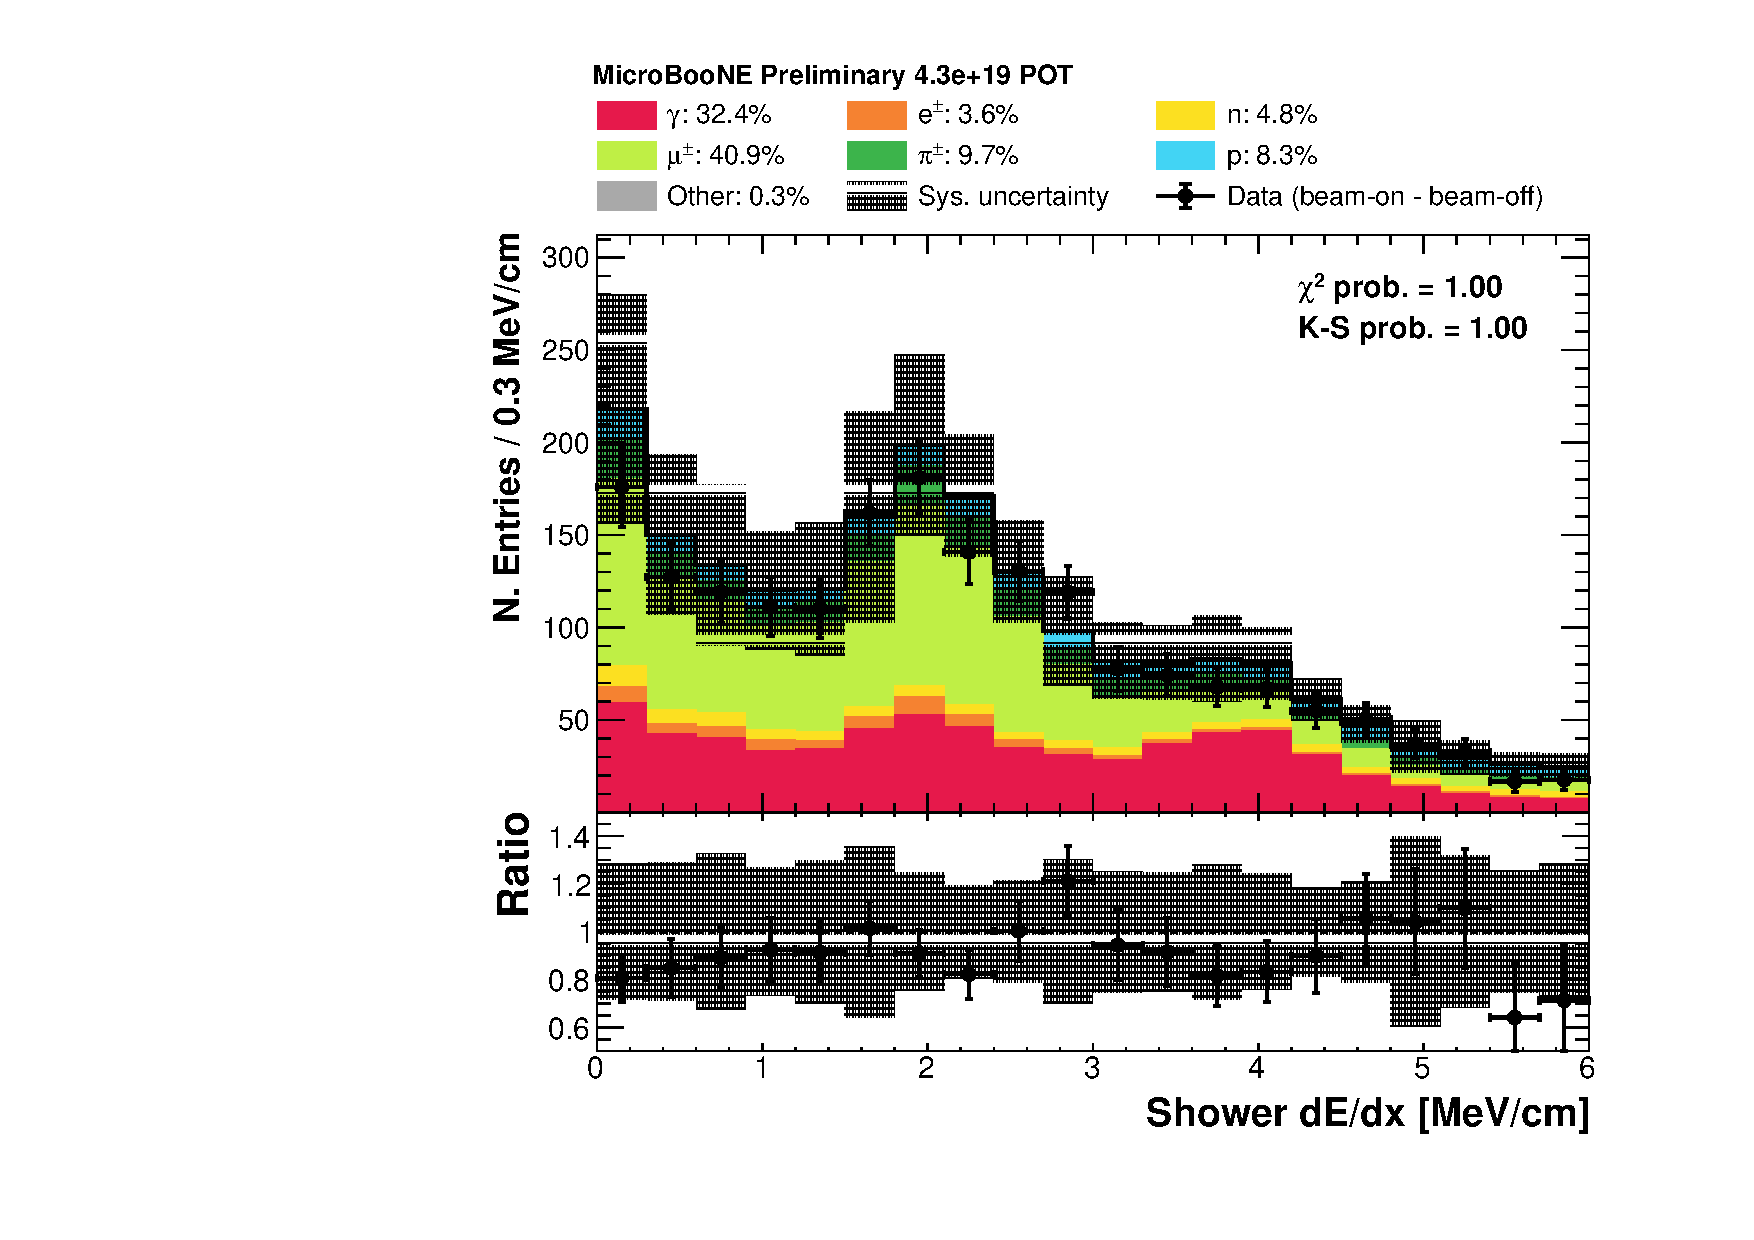
\includegraphics[width=\linewidth]{figures/h_shower_dedx_cali_pdg.pdf}
    \caption{POT normalised, generating particle.} \label{fig:dedx_pdg}
  \end{subfigure}
  \caption{Area and POT normalised distributions of the $dE/dx$ of the reconstructed showers, classified according to the event category and to the primary particle generating the shower.}
\end{figure}

\begin{figure}[htbp]
\centering
  \begin{subfigure}{0.49\textwidth}
    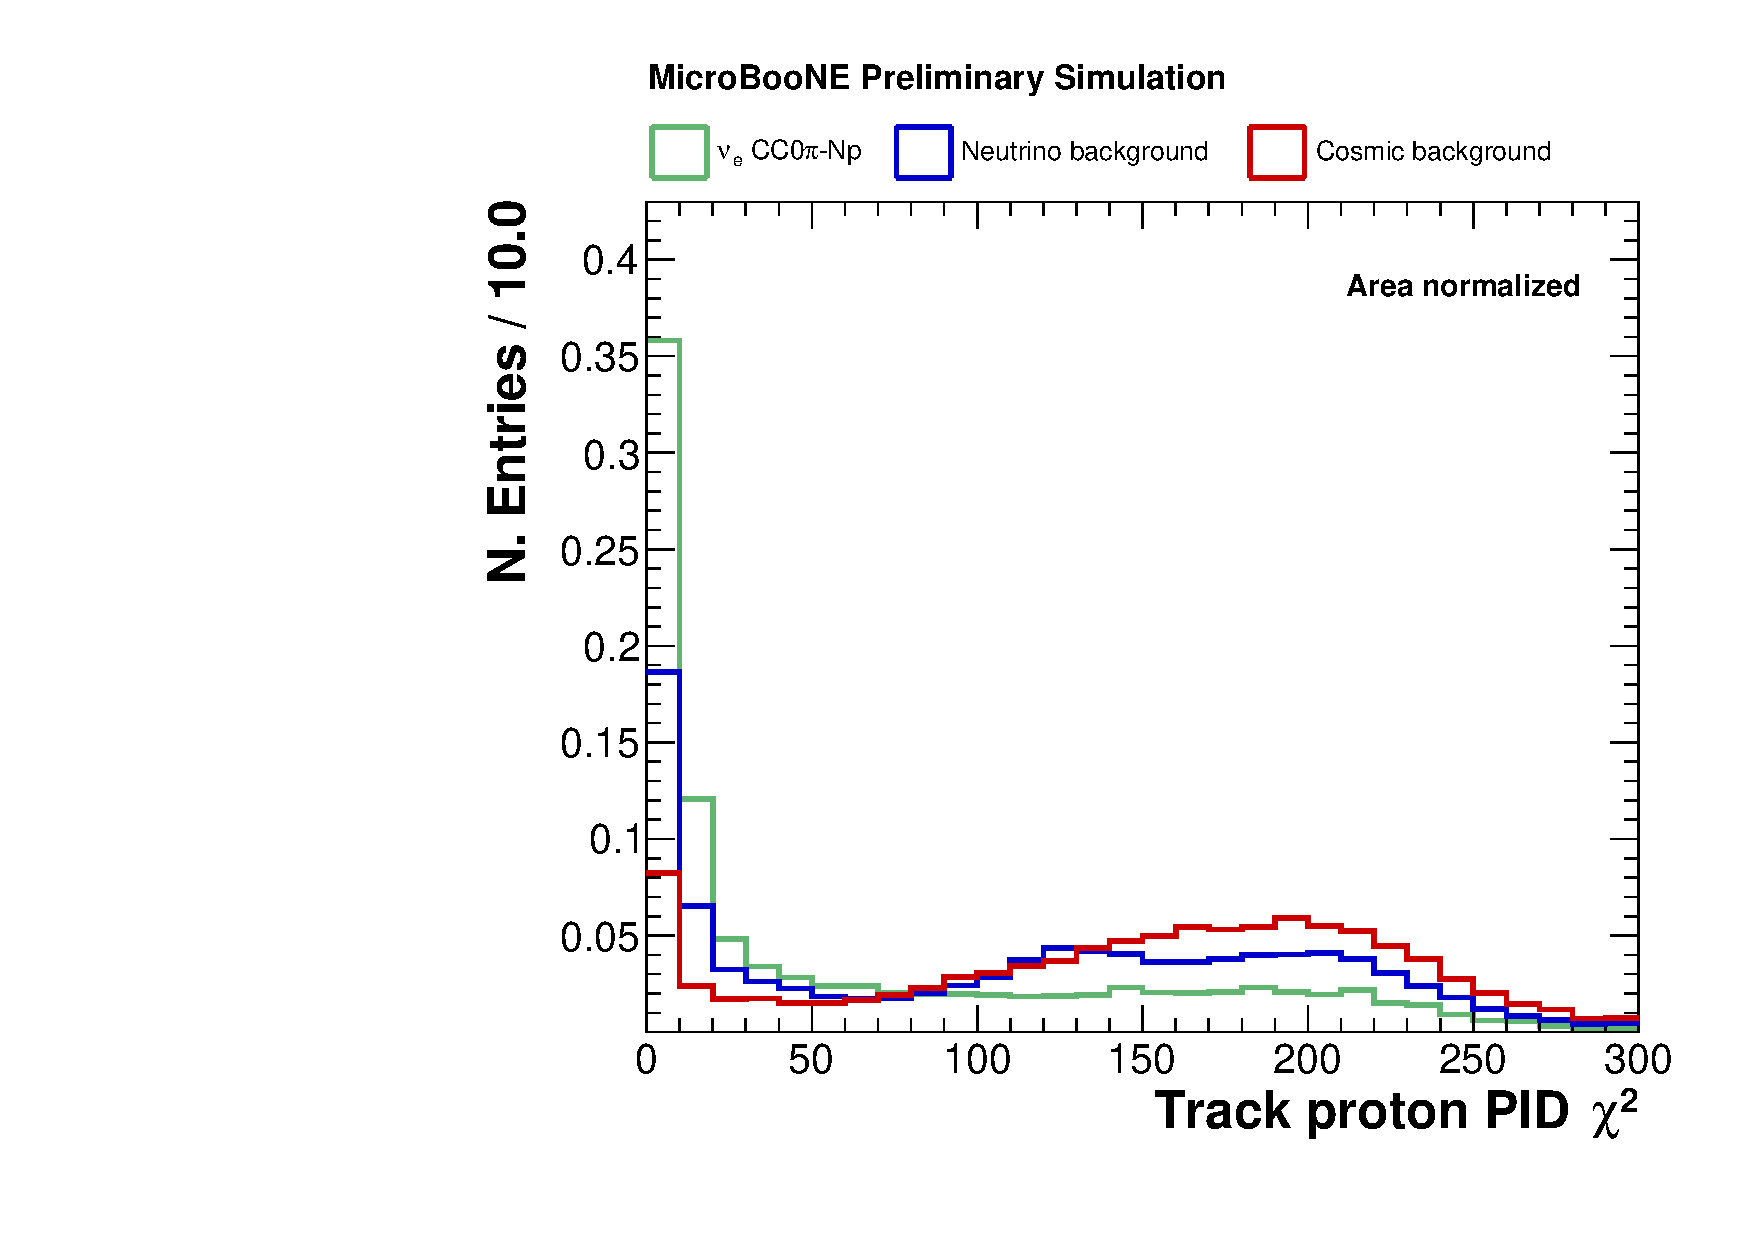
\includegraphics[width=\linewidth]{figures/h_track_pidchipr_norm.pdf}
    \caption{Area normalised.} \label{fig:proton_norm}
  \end{subfigure}
    \begin{subfigure}{0.49\textwidth}
    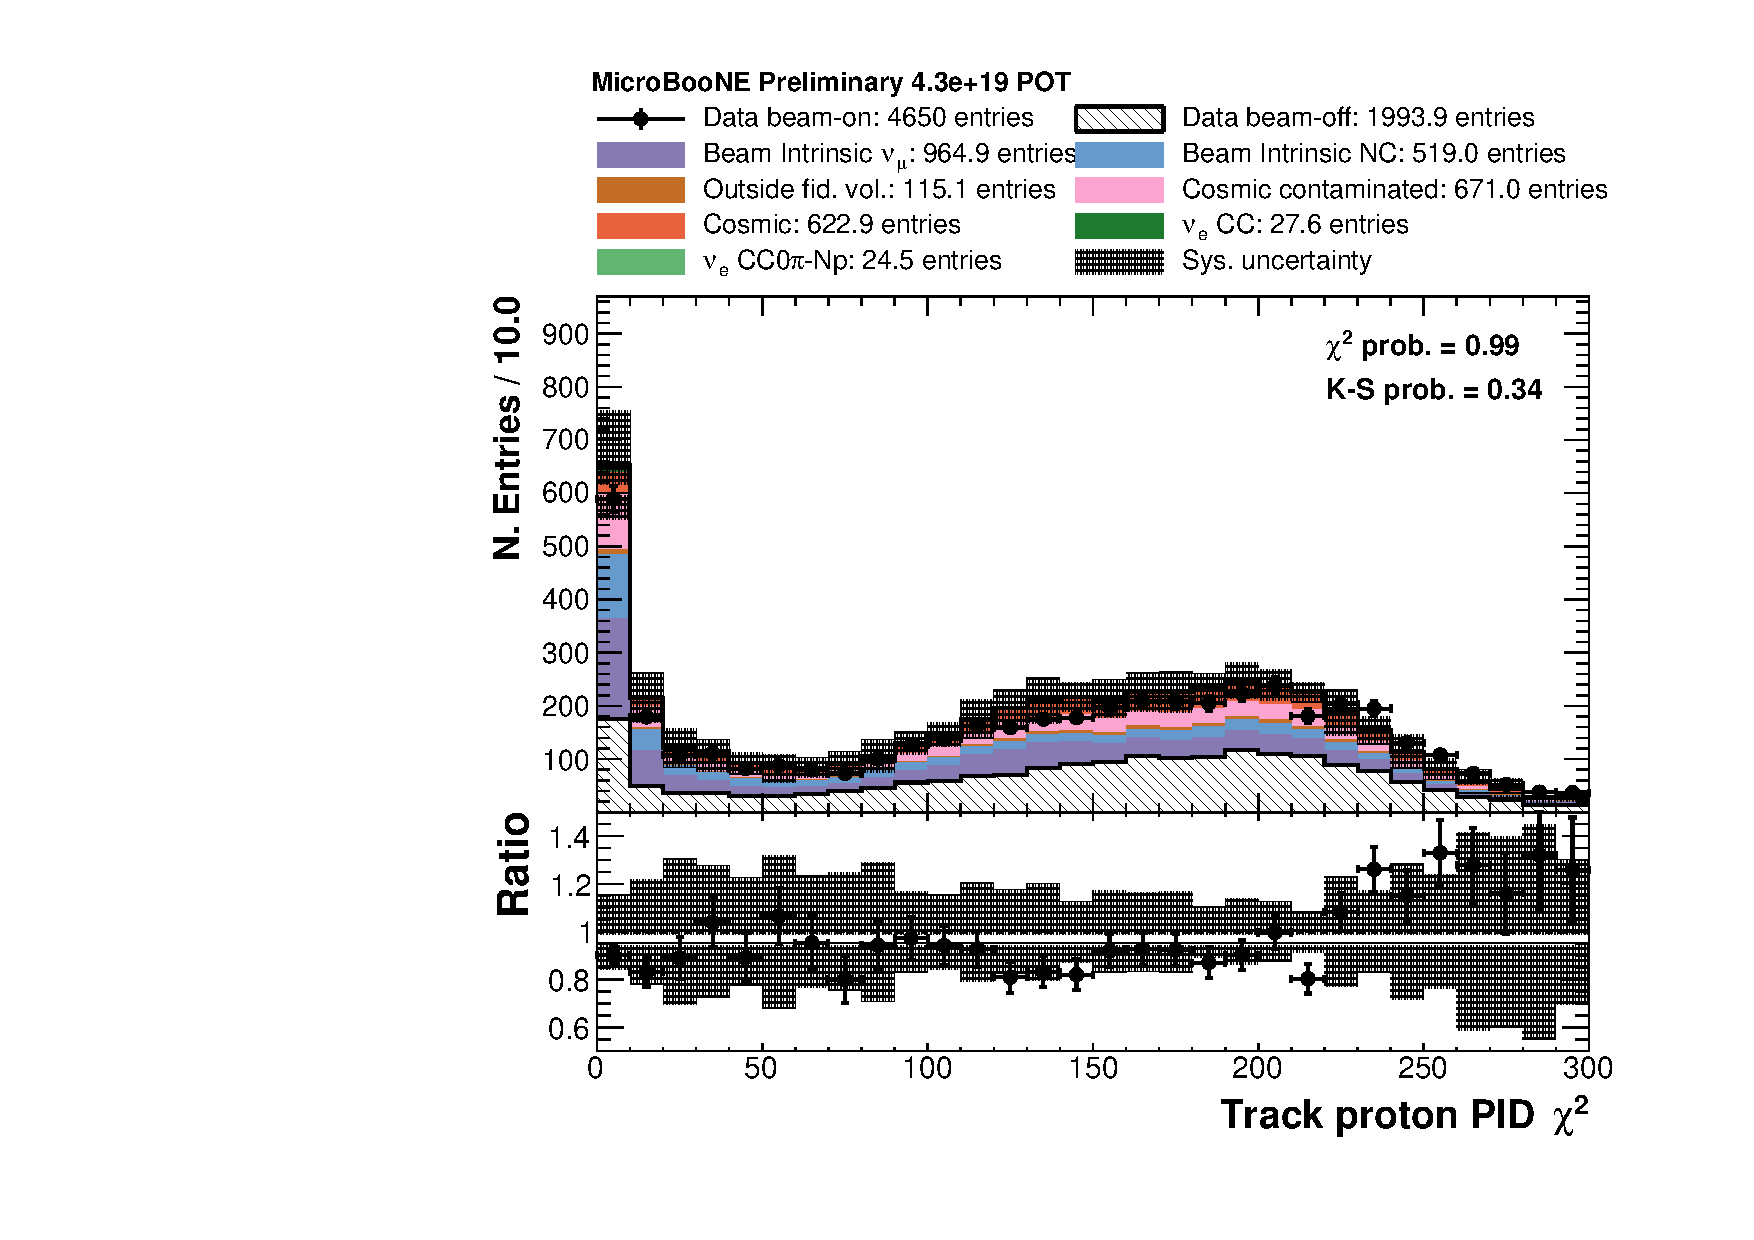
\includegraphics[width=\linewidth]{figures/h_track_pidchipr.pdf}
    \caption{POT normalised, event category.} \label{fig:proton_pot}
  \end{subfigure}
  \begin{subfigure}{0.49\textwidth}
    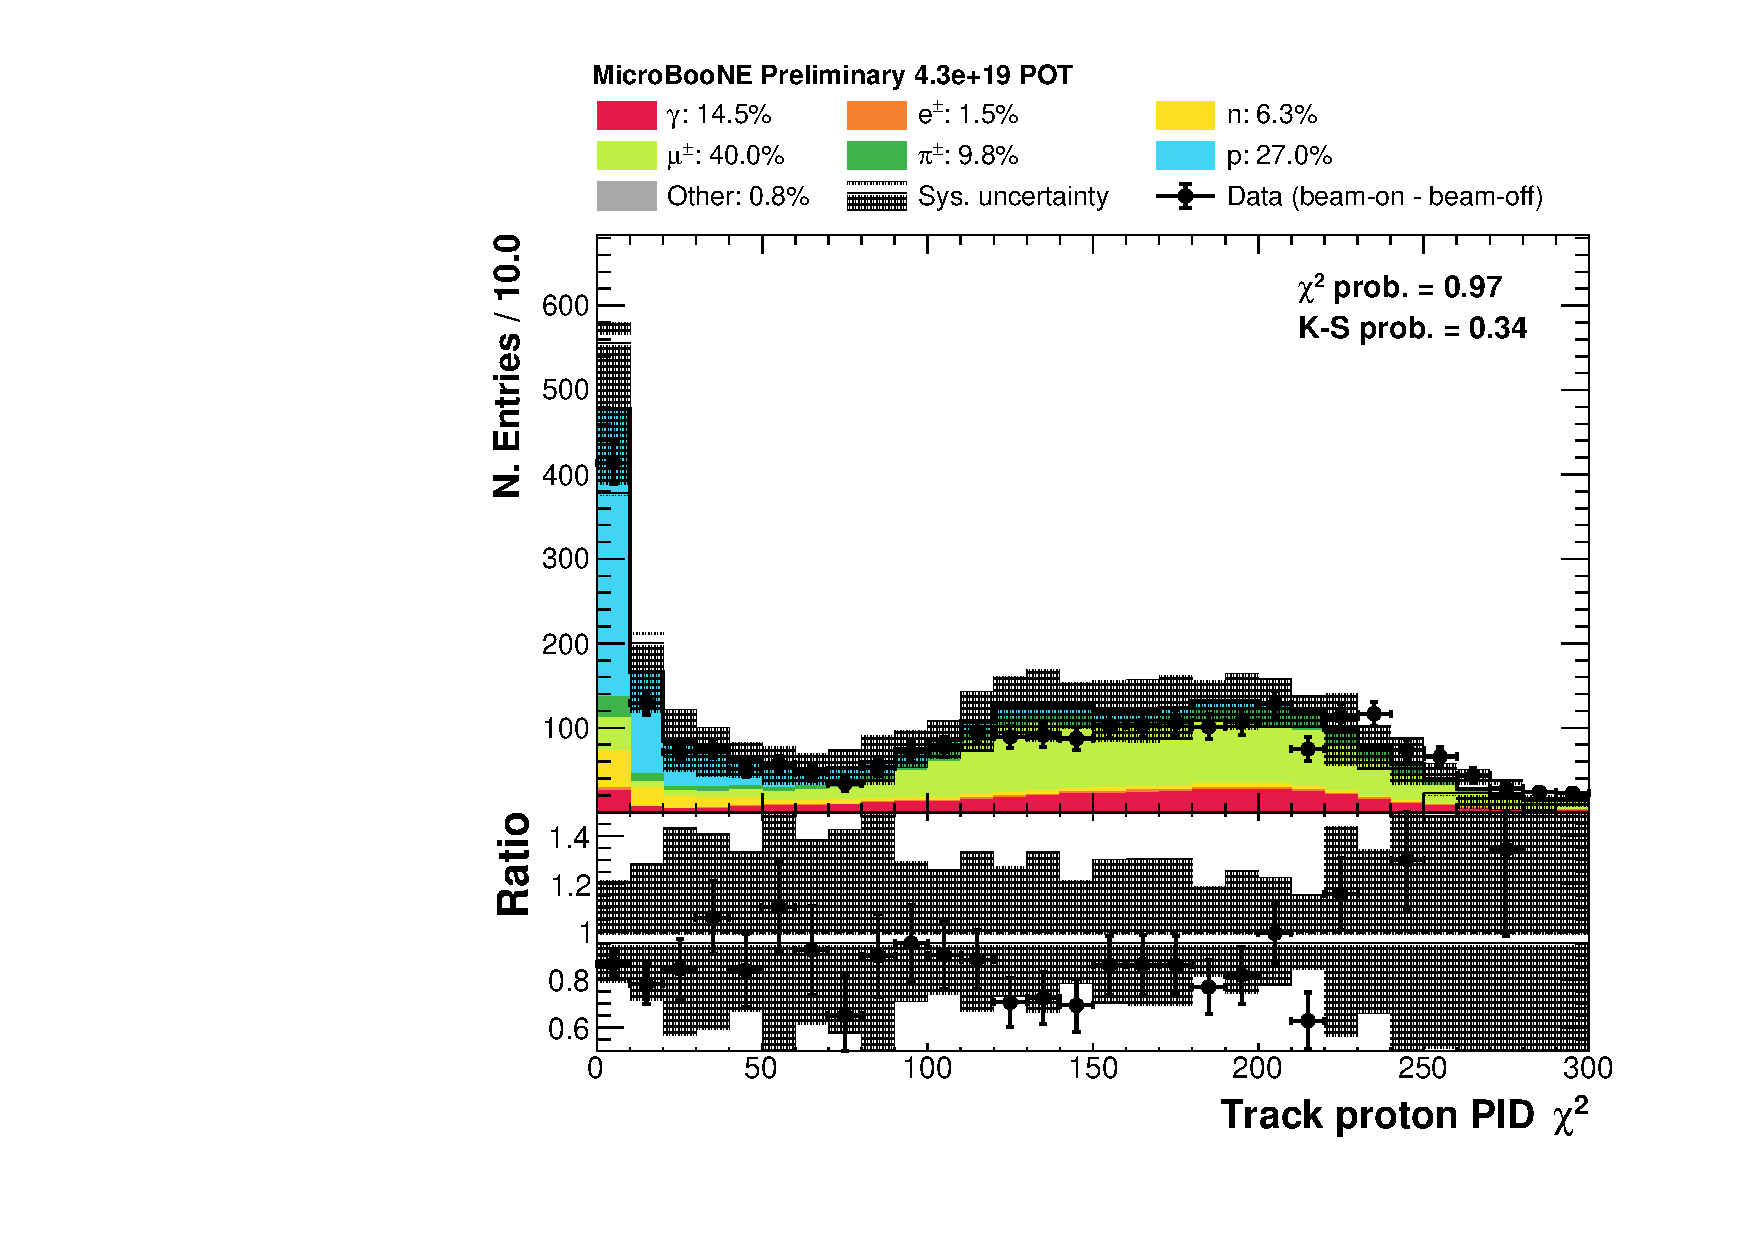
\includegraphics[width=\linewidth]{figures/h_track_pidchipr_pdg.pdf}
    \caption{POT normalised, generating particle.} \label{fig:proton_pdg}
  \end{subfigure}
  \caption{Area and POT normalised distributions of the proton $\chi^2$ score of the reconstructed tracks, classified according to the event category and to the primary particle generating the shower.}
\end{figure}

\begin{figure}[htbp]
\centering
  \begin{subfigure}{0.49\textwidth}
    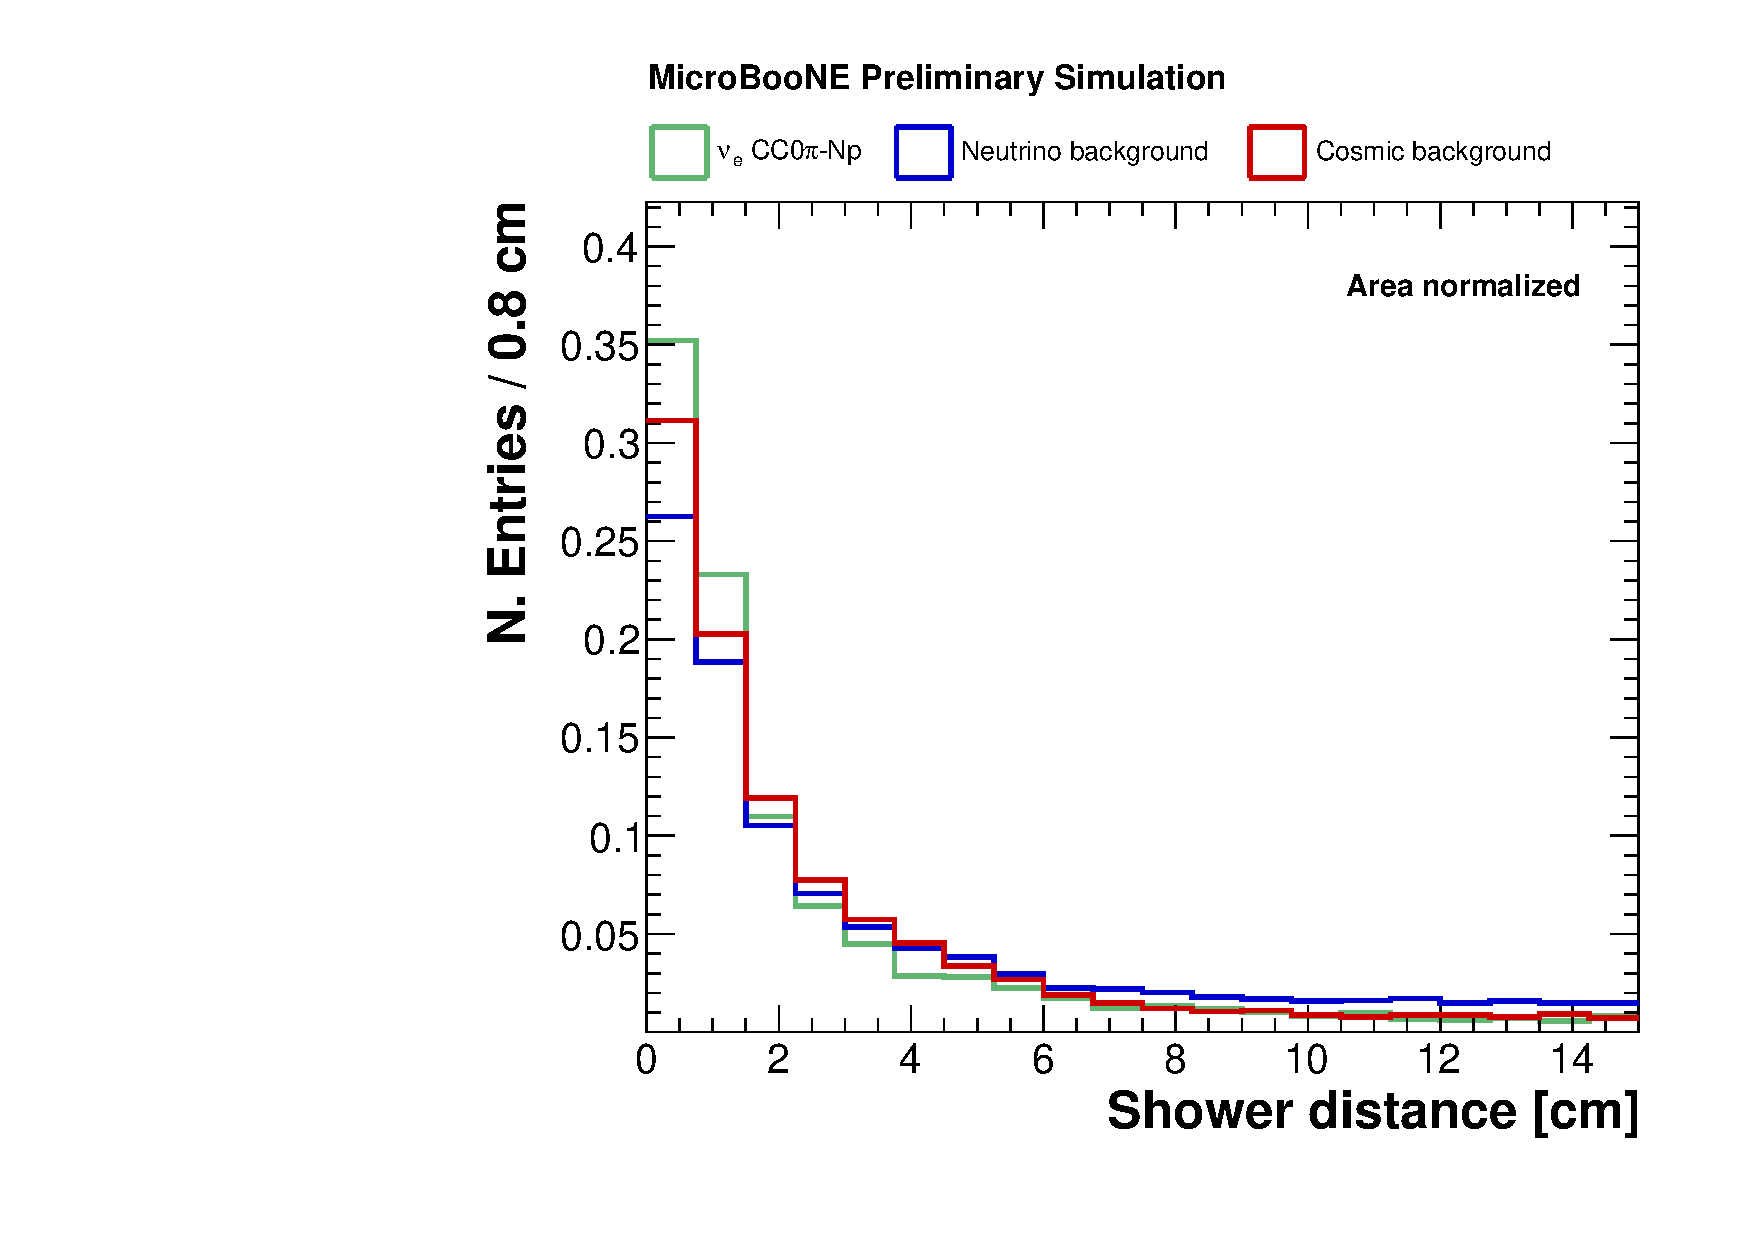
\includegraphics[width=\linewidth]{figures/h_shower_distance_norm.pdf}
    \caption{Area normalised.} \label{fig:showerd_norm}
  \end{subfigure}
    \begin{subfigure}{0.49\textwidth}
    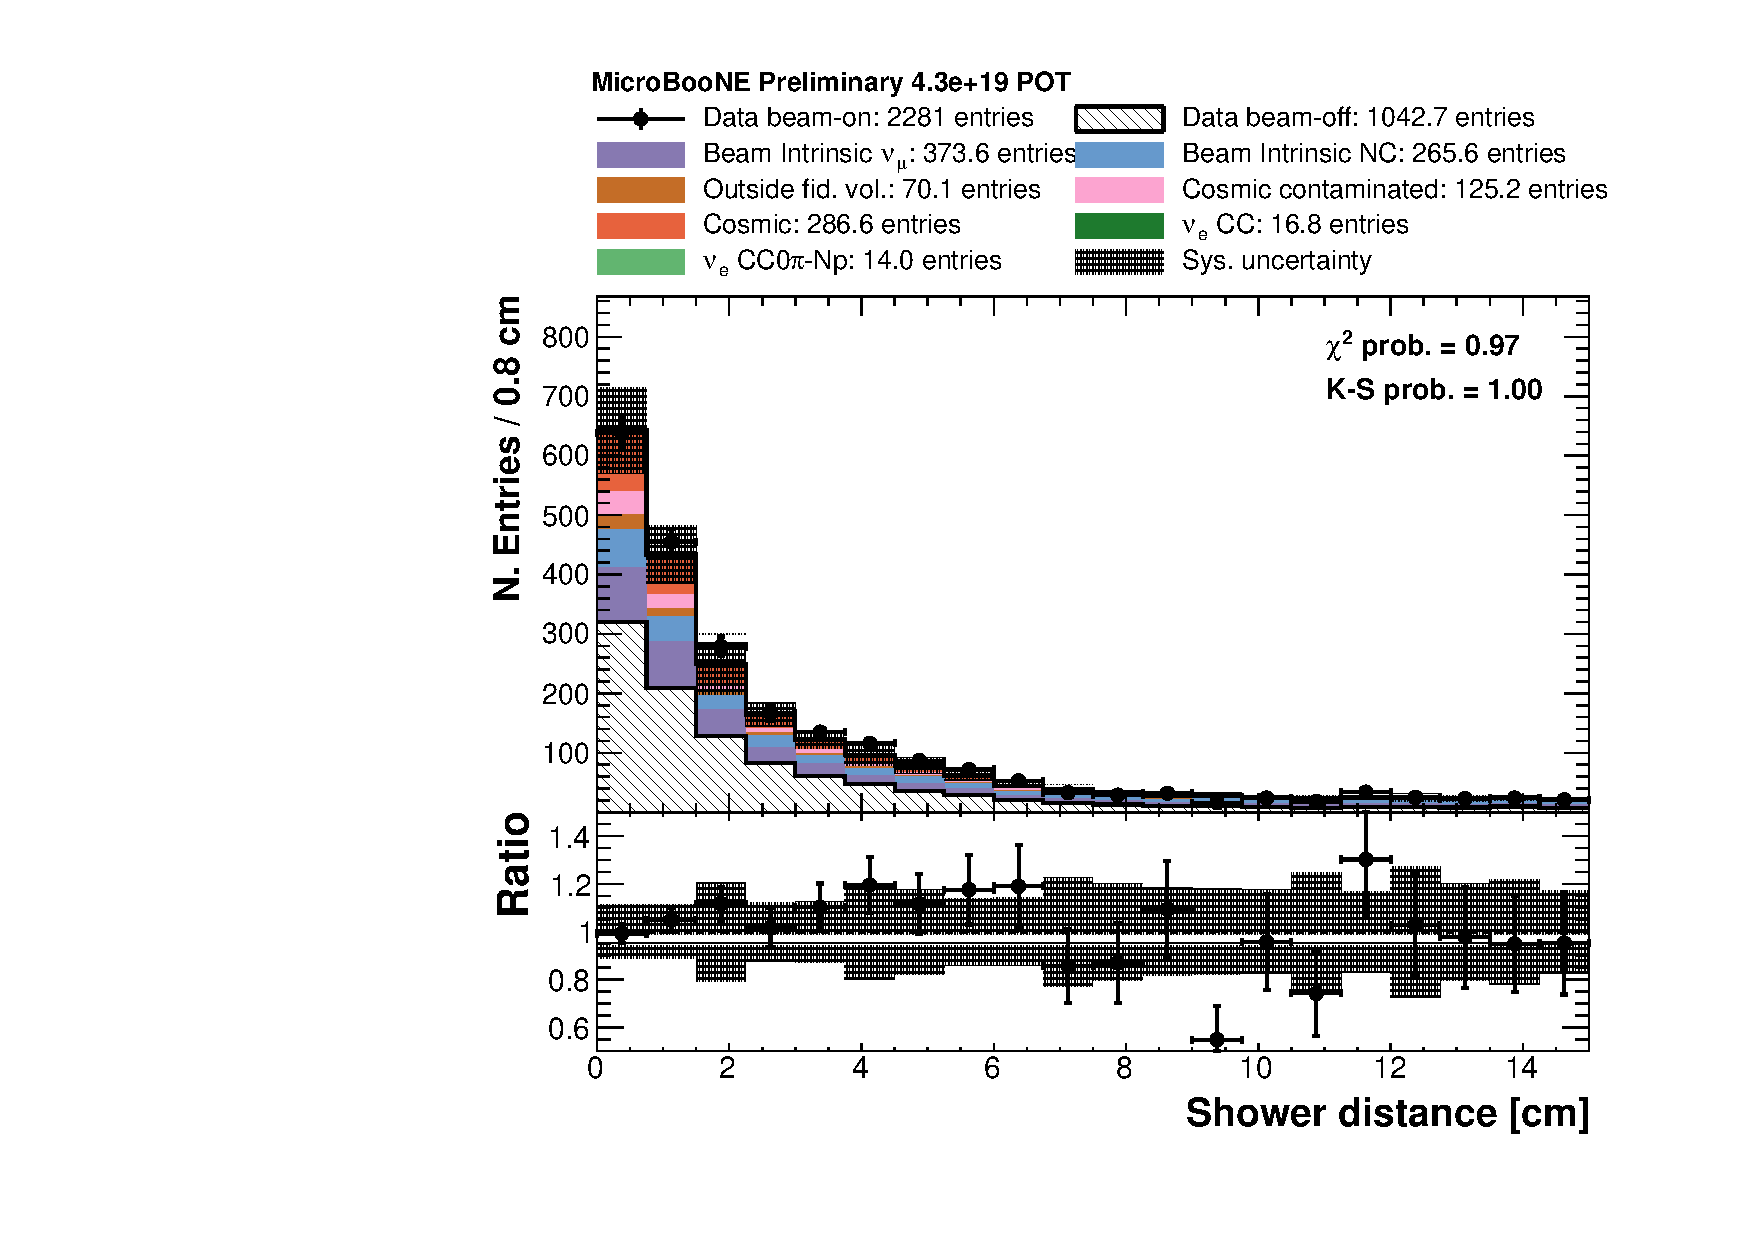
\includegraphics[width=\linewidth]{figures/h_shower_distance.pdf}
    \caption{POT normalised, event category.} \label{fig:showerd_pot}
  \end{subfigure}
  \begin{subfigure}{0.49\textwidth}
    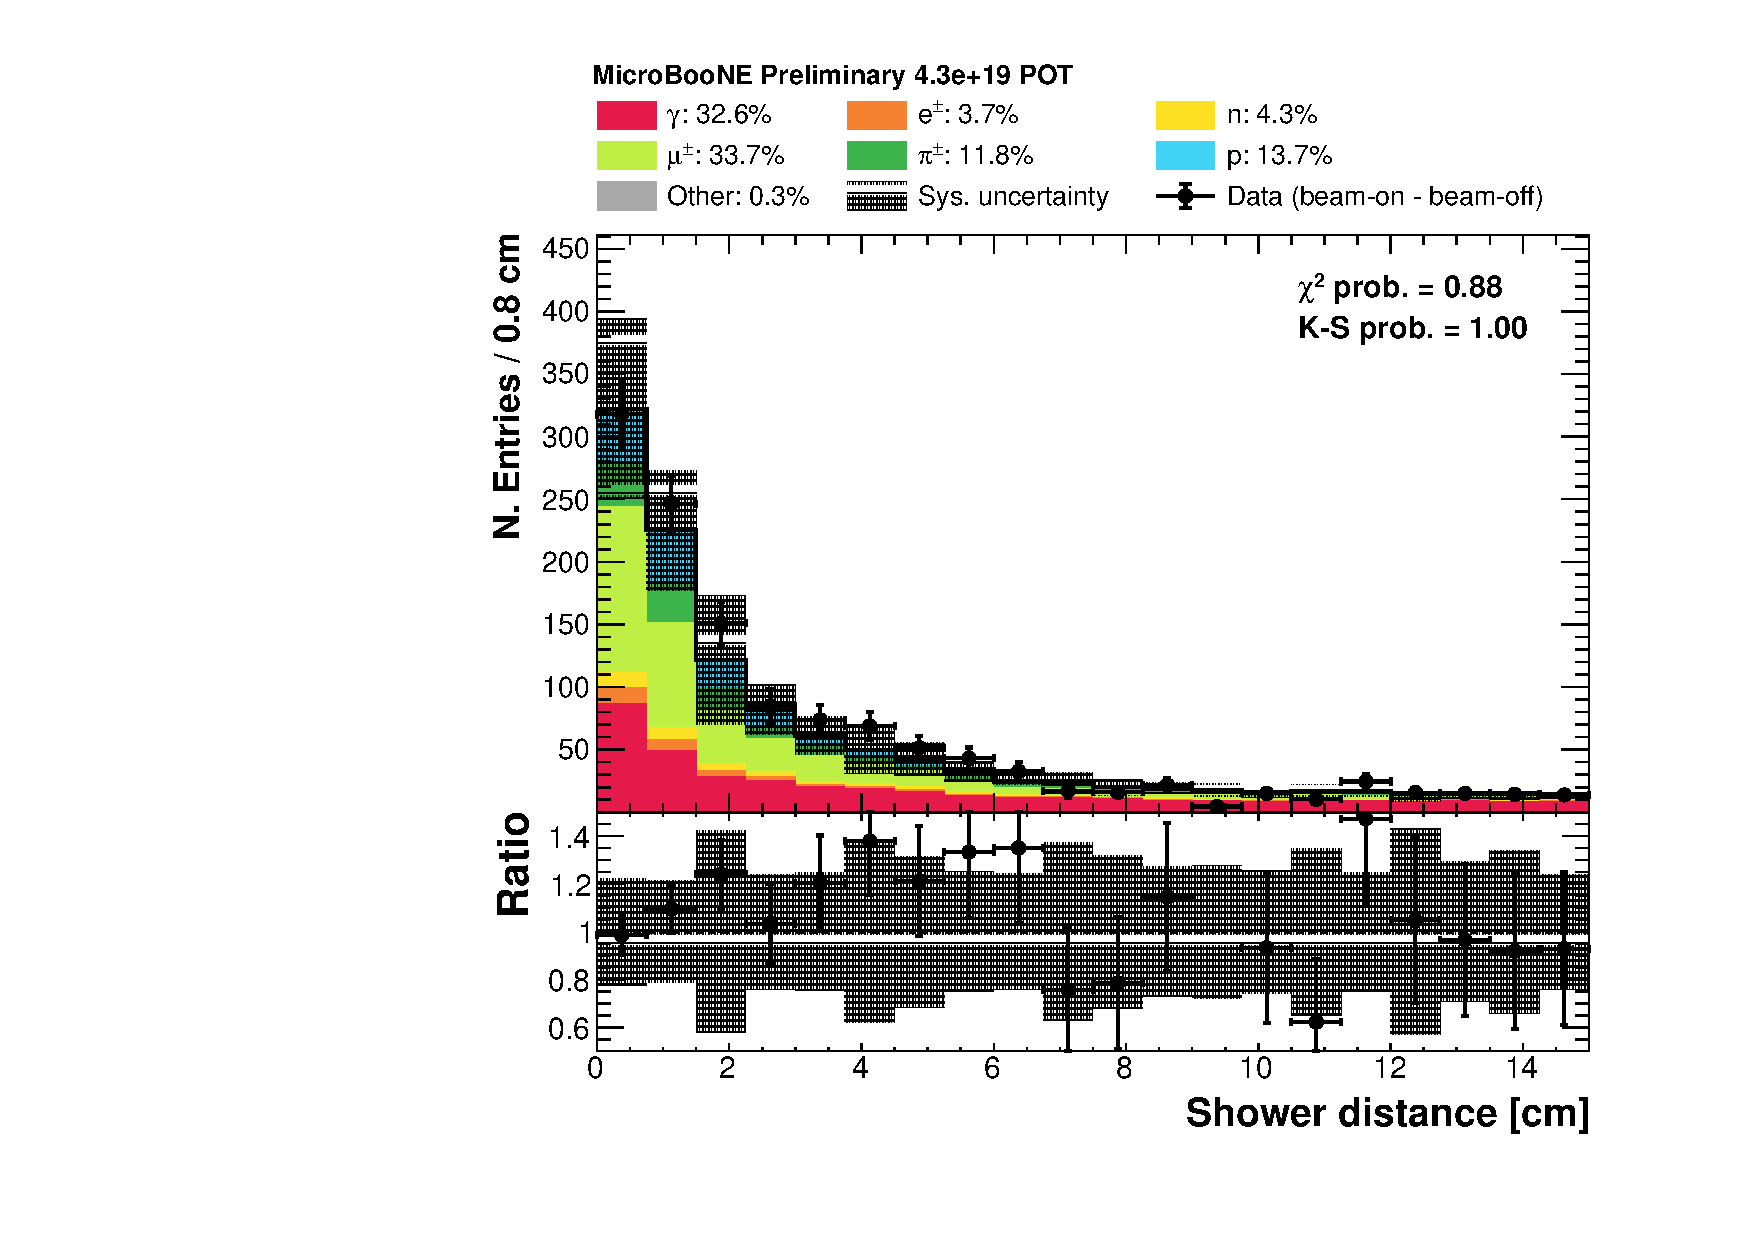
\includegraphics[width=\linewidth]{figures/h_shower_distance_pdg.pdf}
    \caption{POT normalised, generating particle.} \label{fig:showerd_pdg}
  \end{subfigure}
  \caption{Area and POT normalised distributions of the distance between the most proton-like track, selected with the proton identification BDT, and the reconstructed neutrino vertex, classified according to the event category and to the primary particle generating the shower.}
\end{figure}

% \begin{figure}[htbp]
% \centering
%   \begin{subfigure}{0.49\textwidth}
%     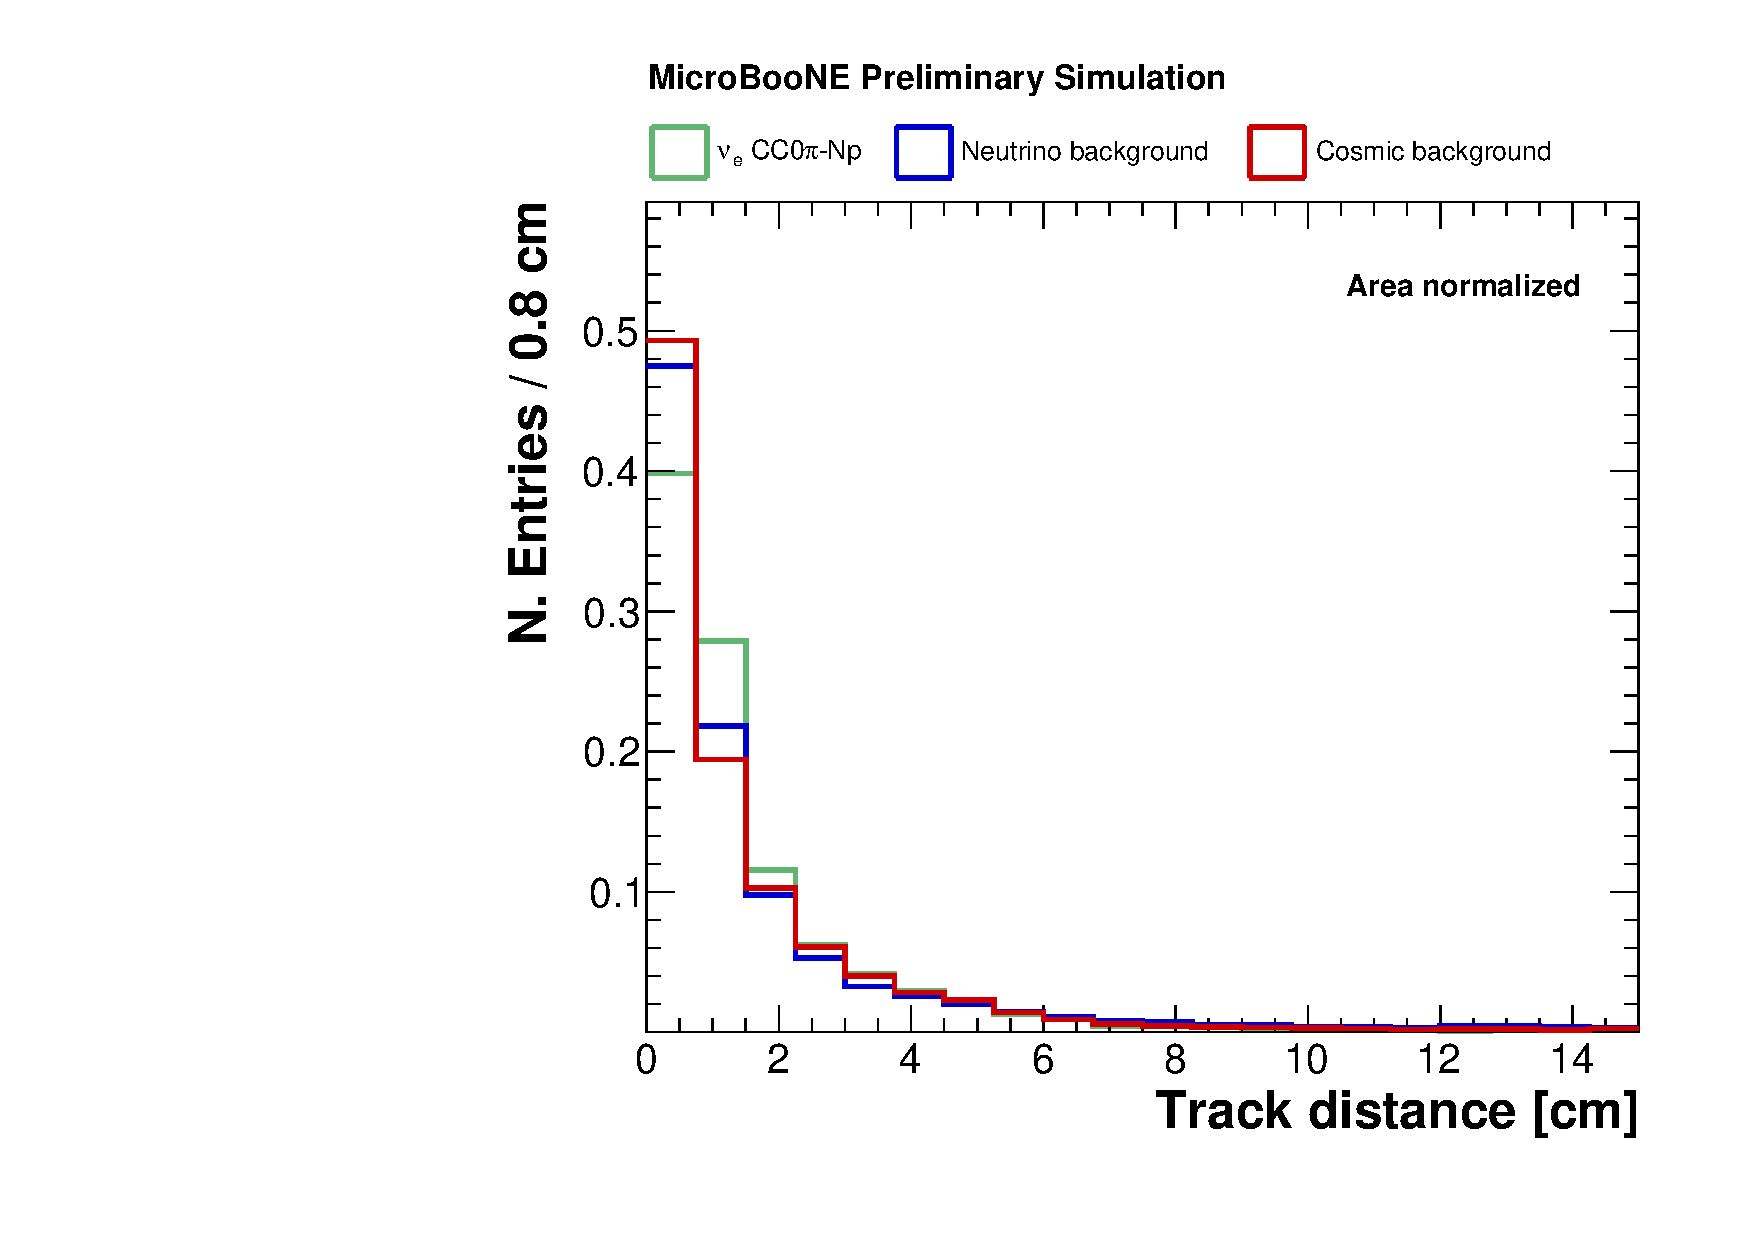
\includegraphics[width=\linewidth]{figures/h_track_distance_norm.pdf}
%     \caption{Area normalised.} \label{fig:shower_norm}
%   \end{subfigure}
%     \begin{subfigure}{0.49\textwidth}
%     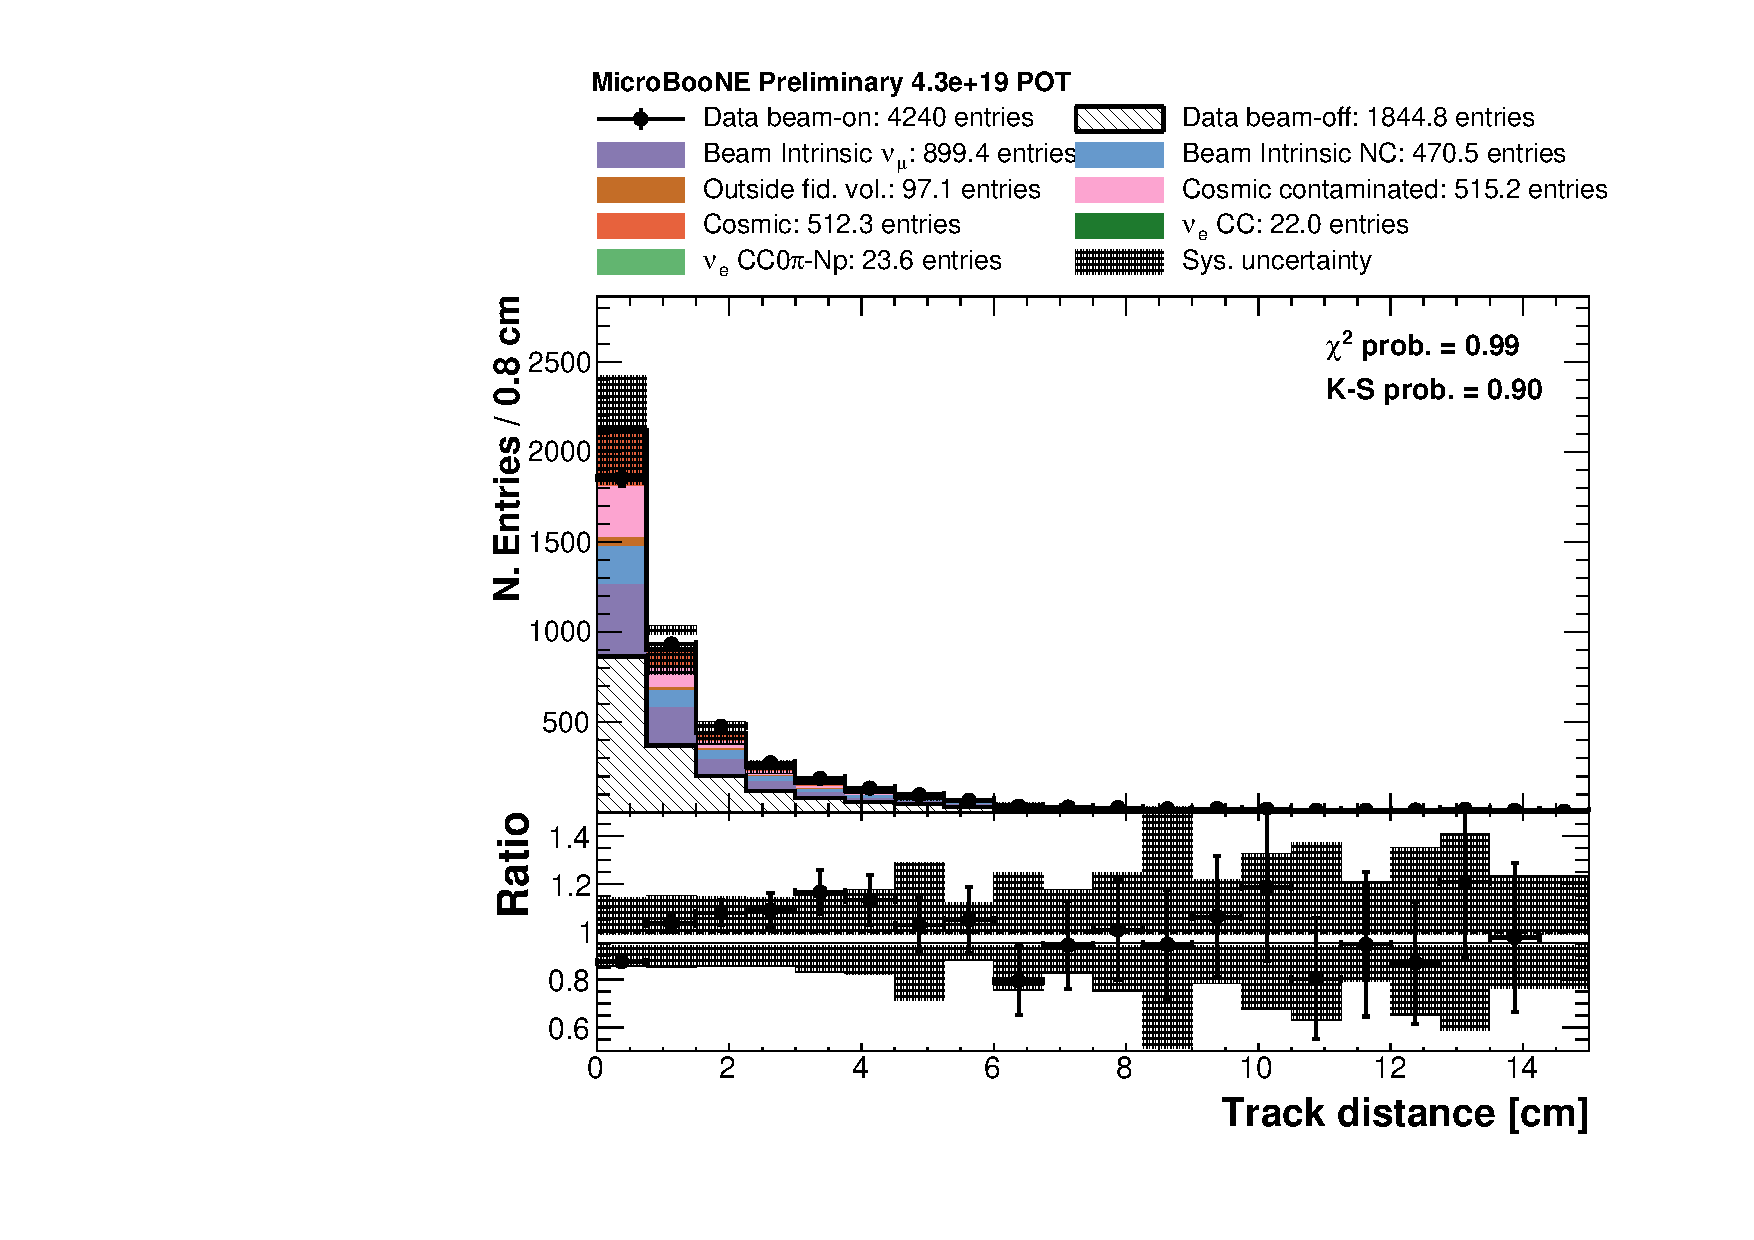
\includegraphics[width=\linewidth]{figures/h_track_distance.pdf}
%     \caption{POT normalised.} \label{fig:shower_pot}
%   \end{subfigure}
%   \caption{Area and POT normalised distributions of the distance between the most energetic shower and the reconstructed neutrino vertex.}
% \end{figure}

\begin{figure}[htbp]
\centering
  \begin{subfigure}{0.49\textwidth}
    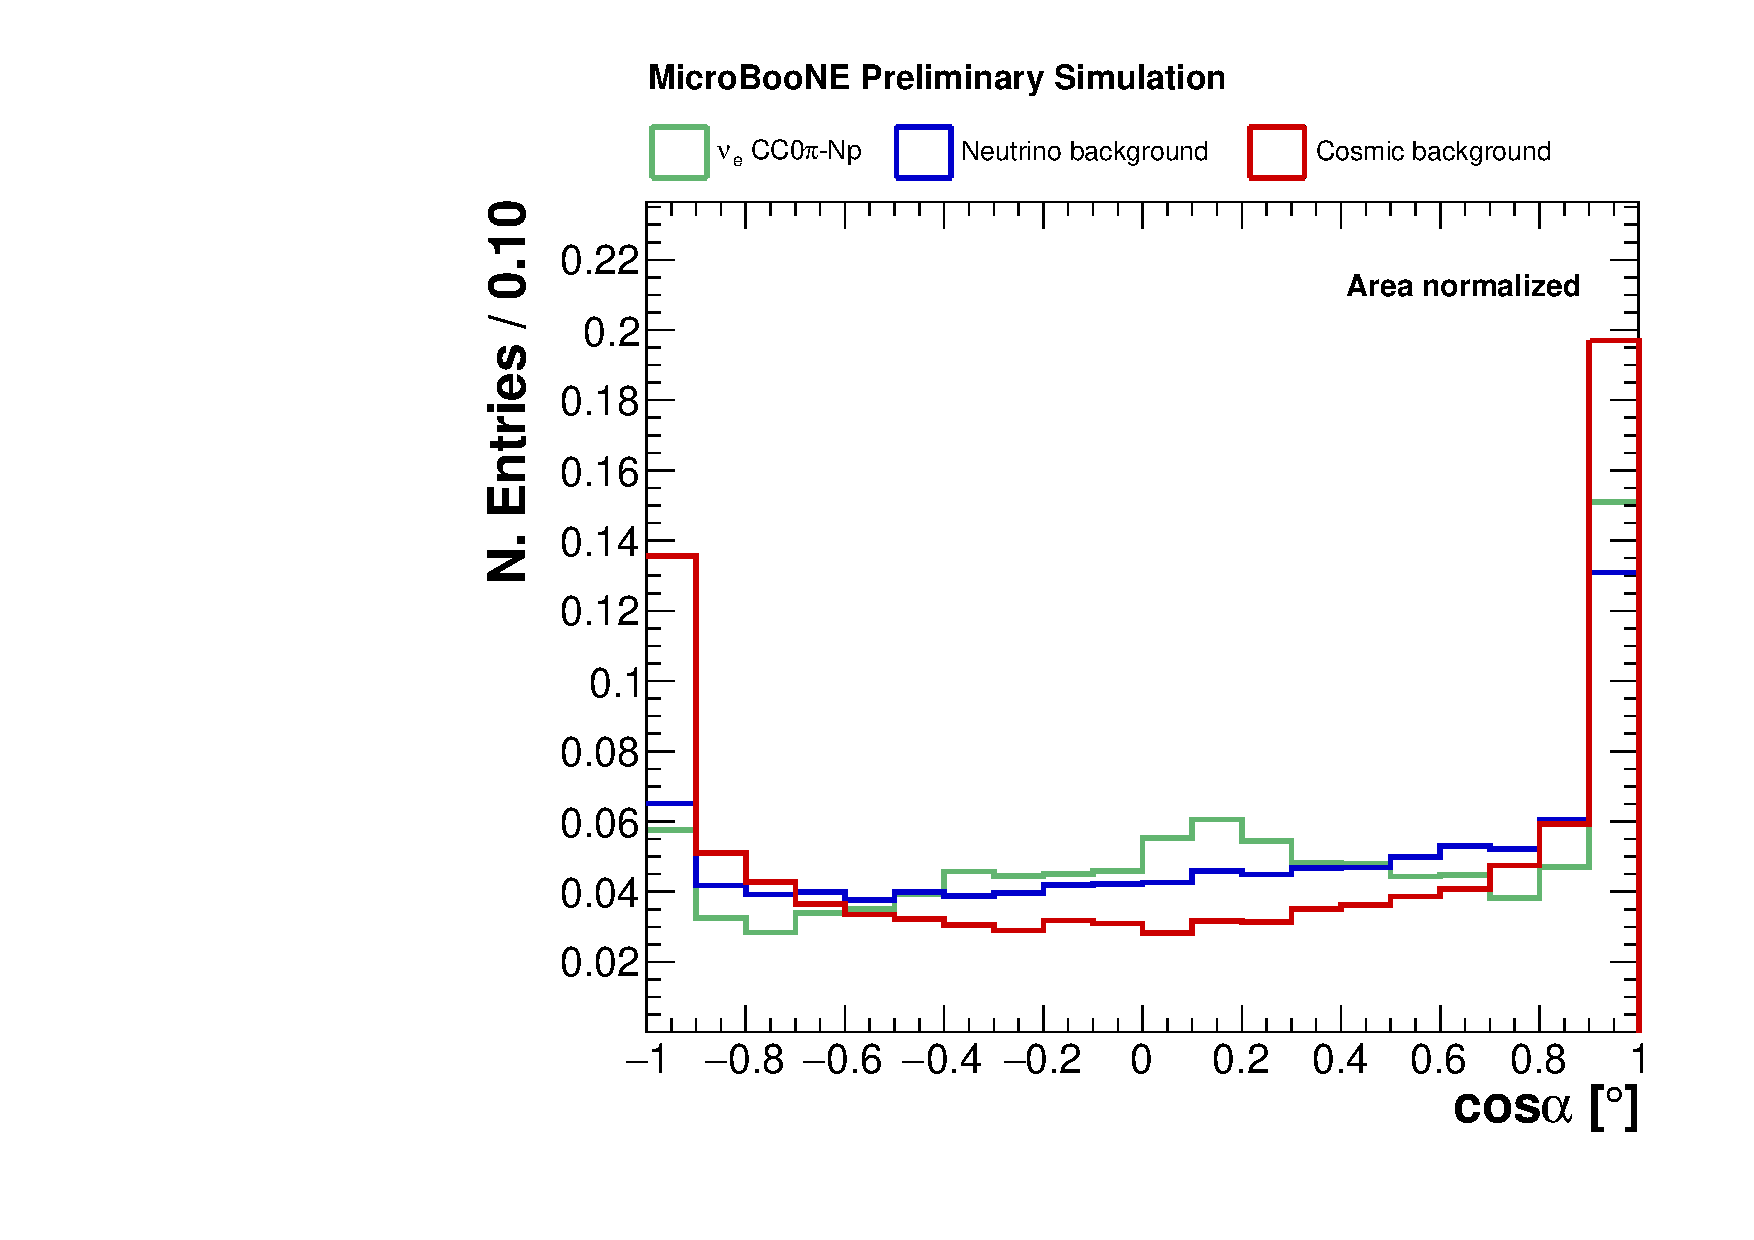
\includegraphics[width=\linewidth]{figures/h_track_shower_angle_norm.pdf}
    \caption{Area normalised.} \label{fig:angle_integral}
  \end{subfigure}
  \begin{subfigure}{0.49\textwidth}
    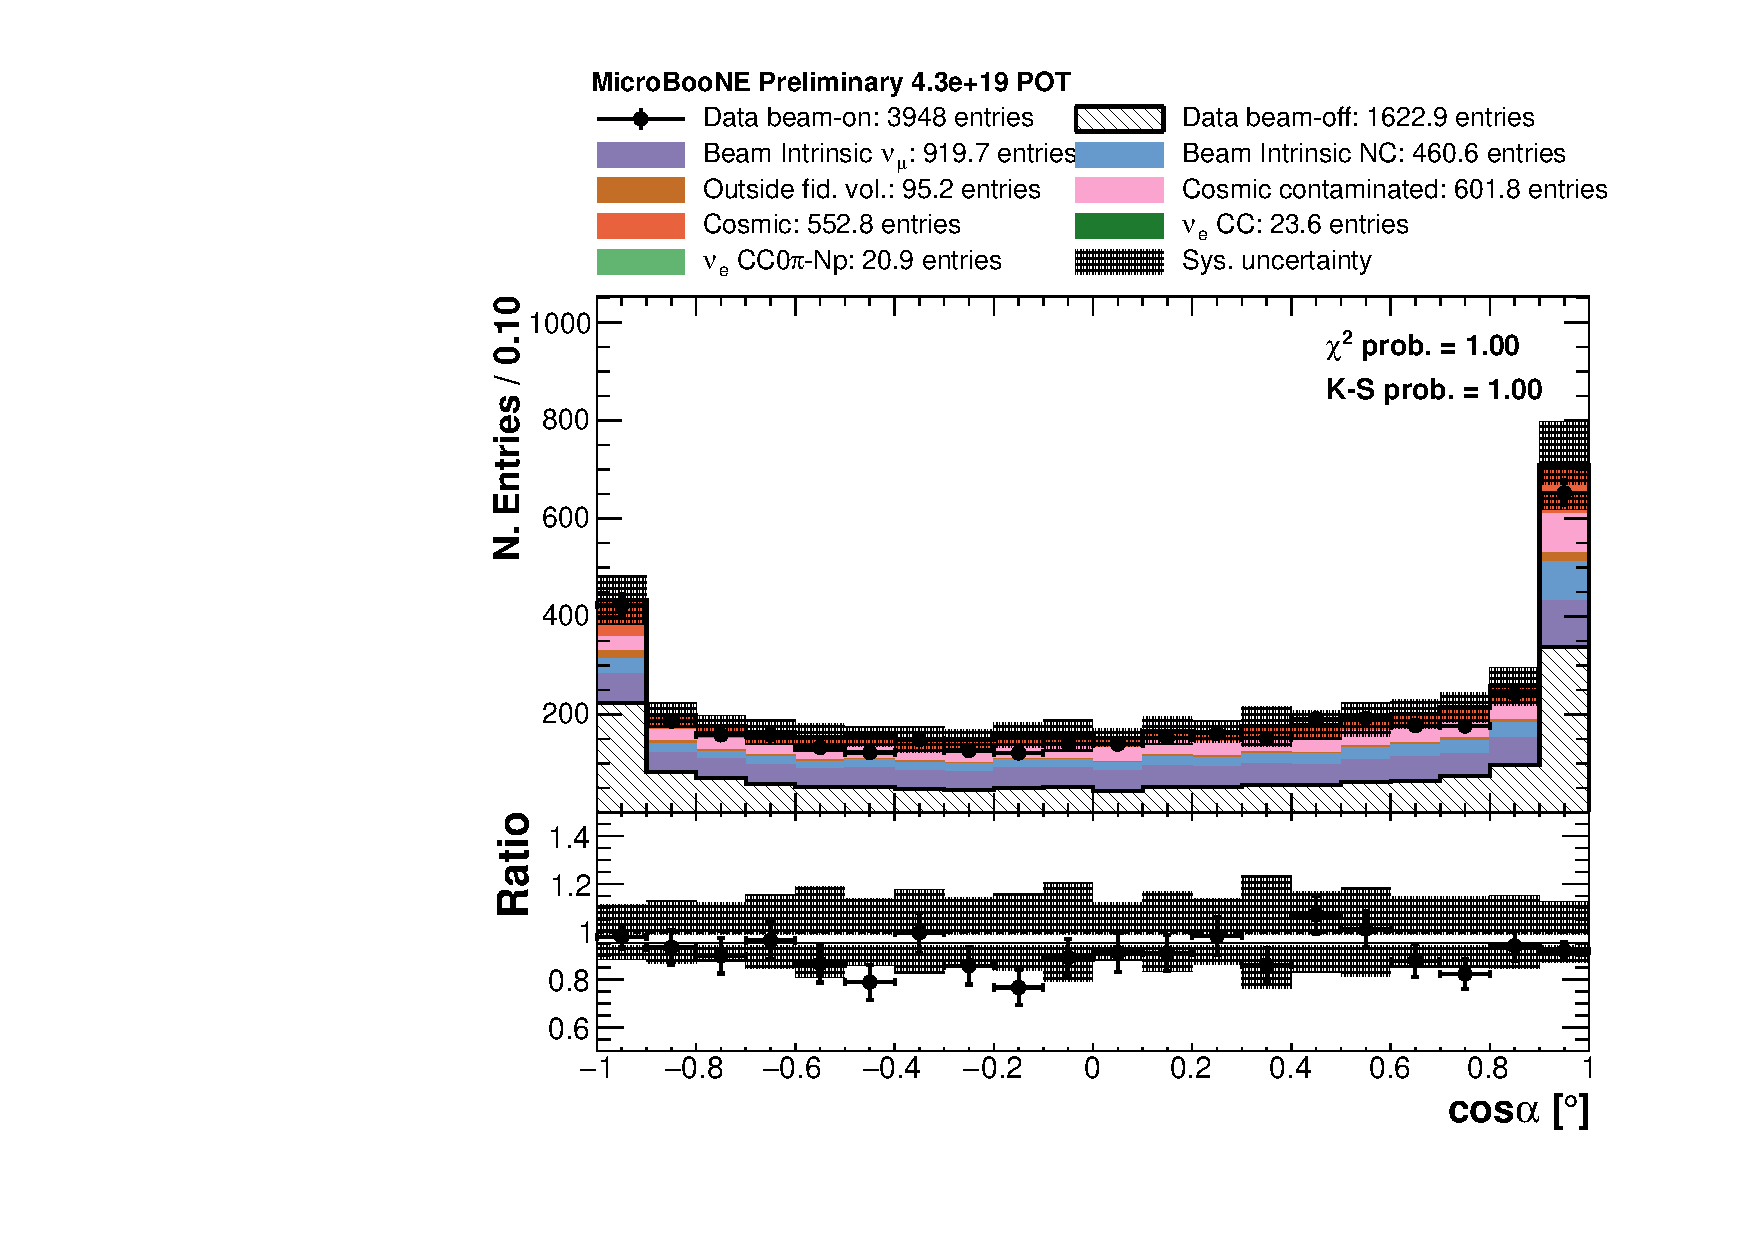
\includegraphics[width=\linewidth]{figures/h_track_shower_angle.pdf}
    \caption{POT normalised, event category.} \label{fig:angle_pot}
  \end{subfigure}
  \begin{subfigure}{0.49\textwidth}
    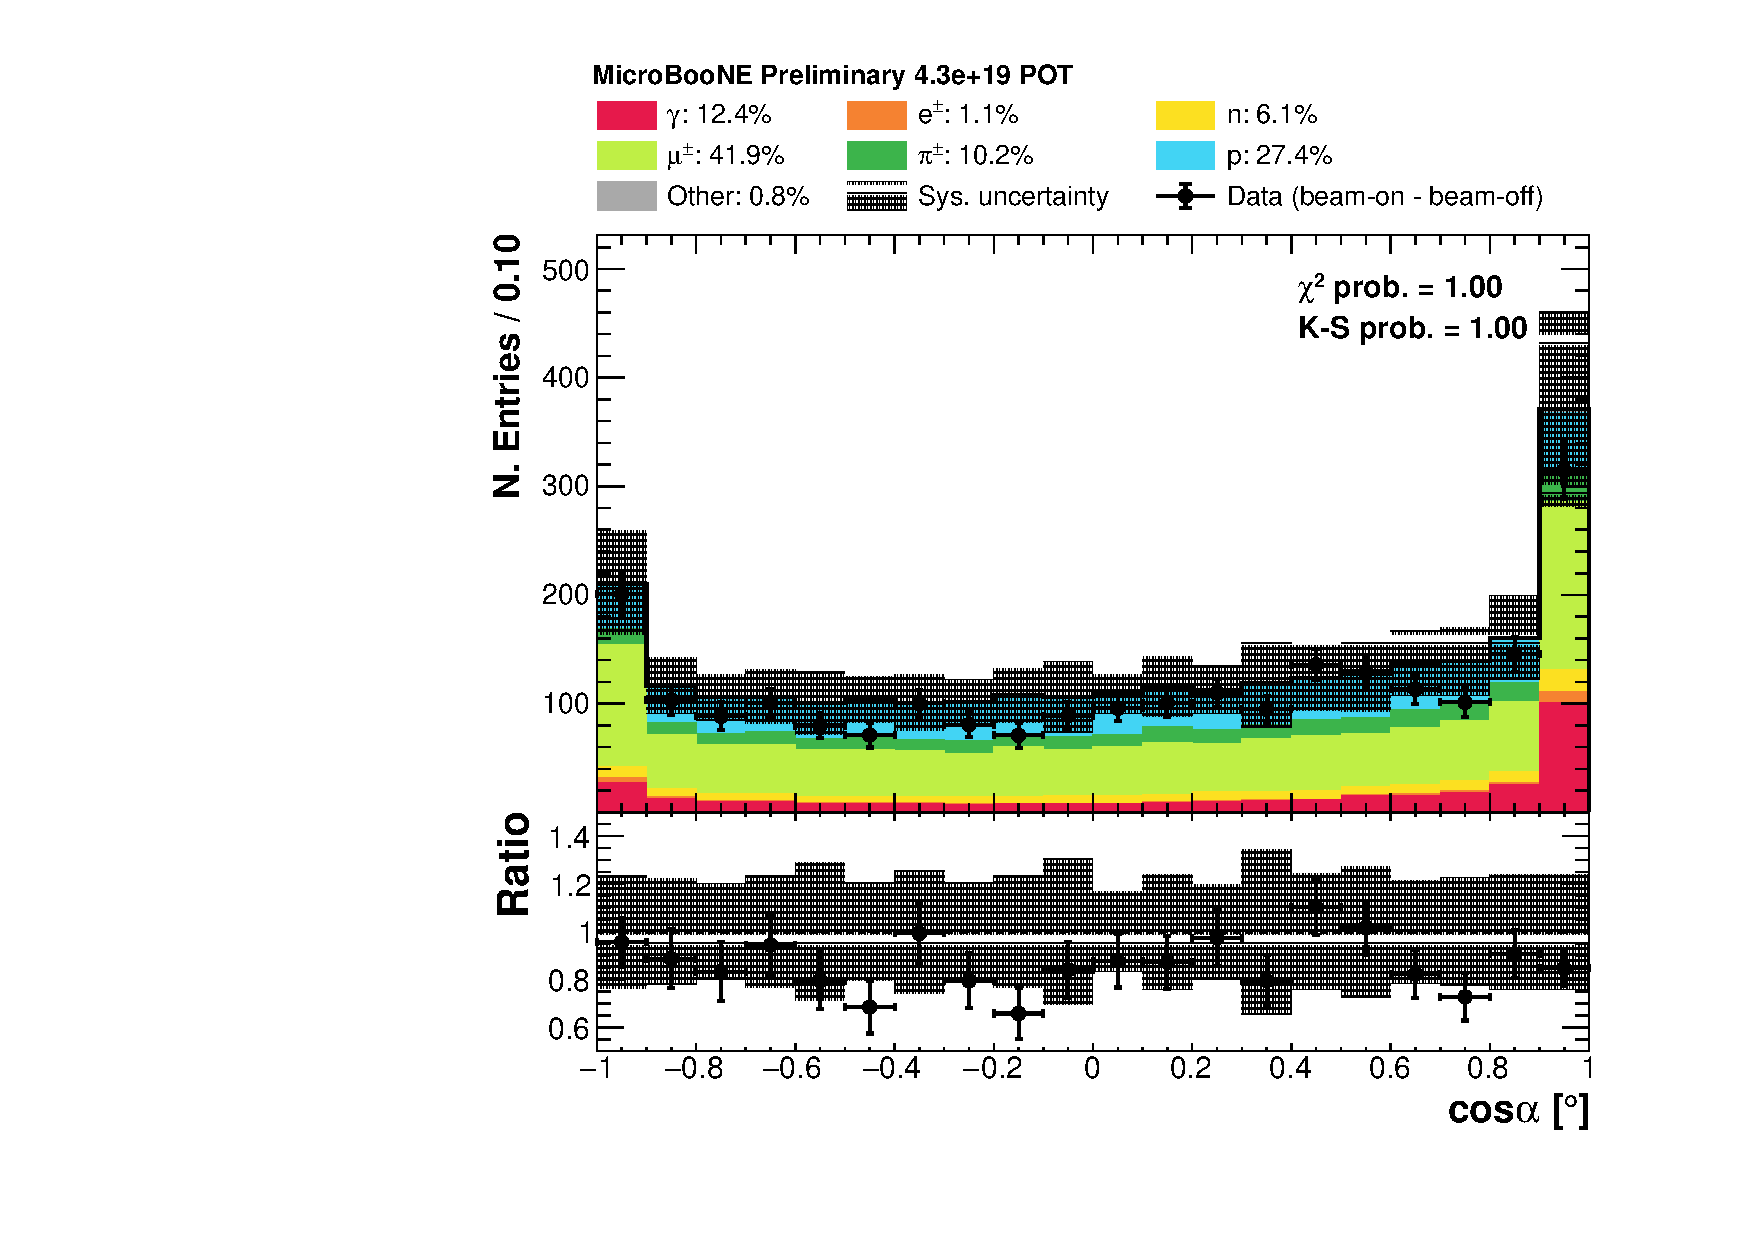
\includegraphics[width=\linewidth]{figures/h_track_shower_angle_pdg.pdf}
    \caption{POT normalised, generating particle.} \label{fig:angle_pdg}
  \end{subfigure}
  \caption{Area and POT normalised distributions of the angle $\alpha$ between each reconstructed track and the leading shower, classified according to the event category and to the primary particle generating the shower.}
\end{figure}

% \begin{figure}[htbp]
% \centering
%   \begin{subfigure}{0.49\textwidth}
%     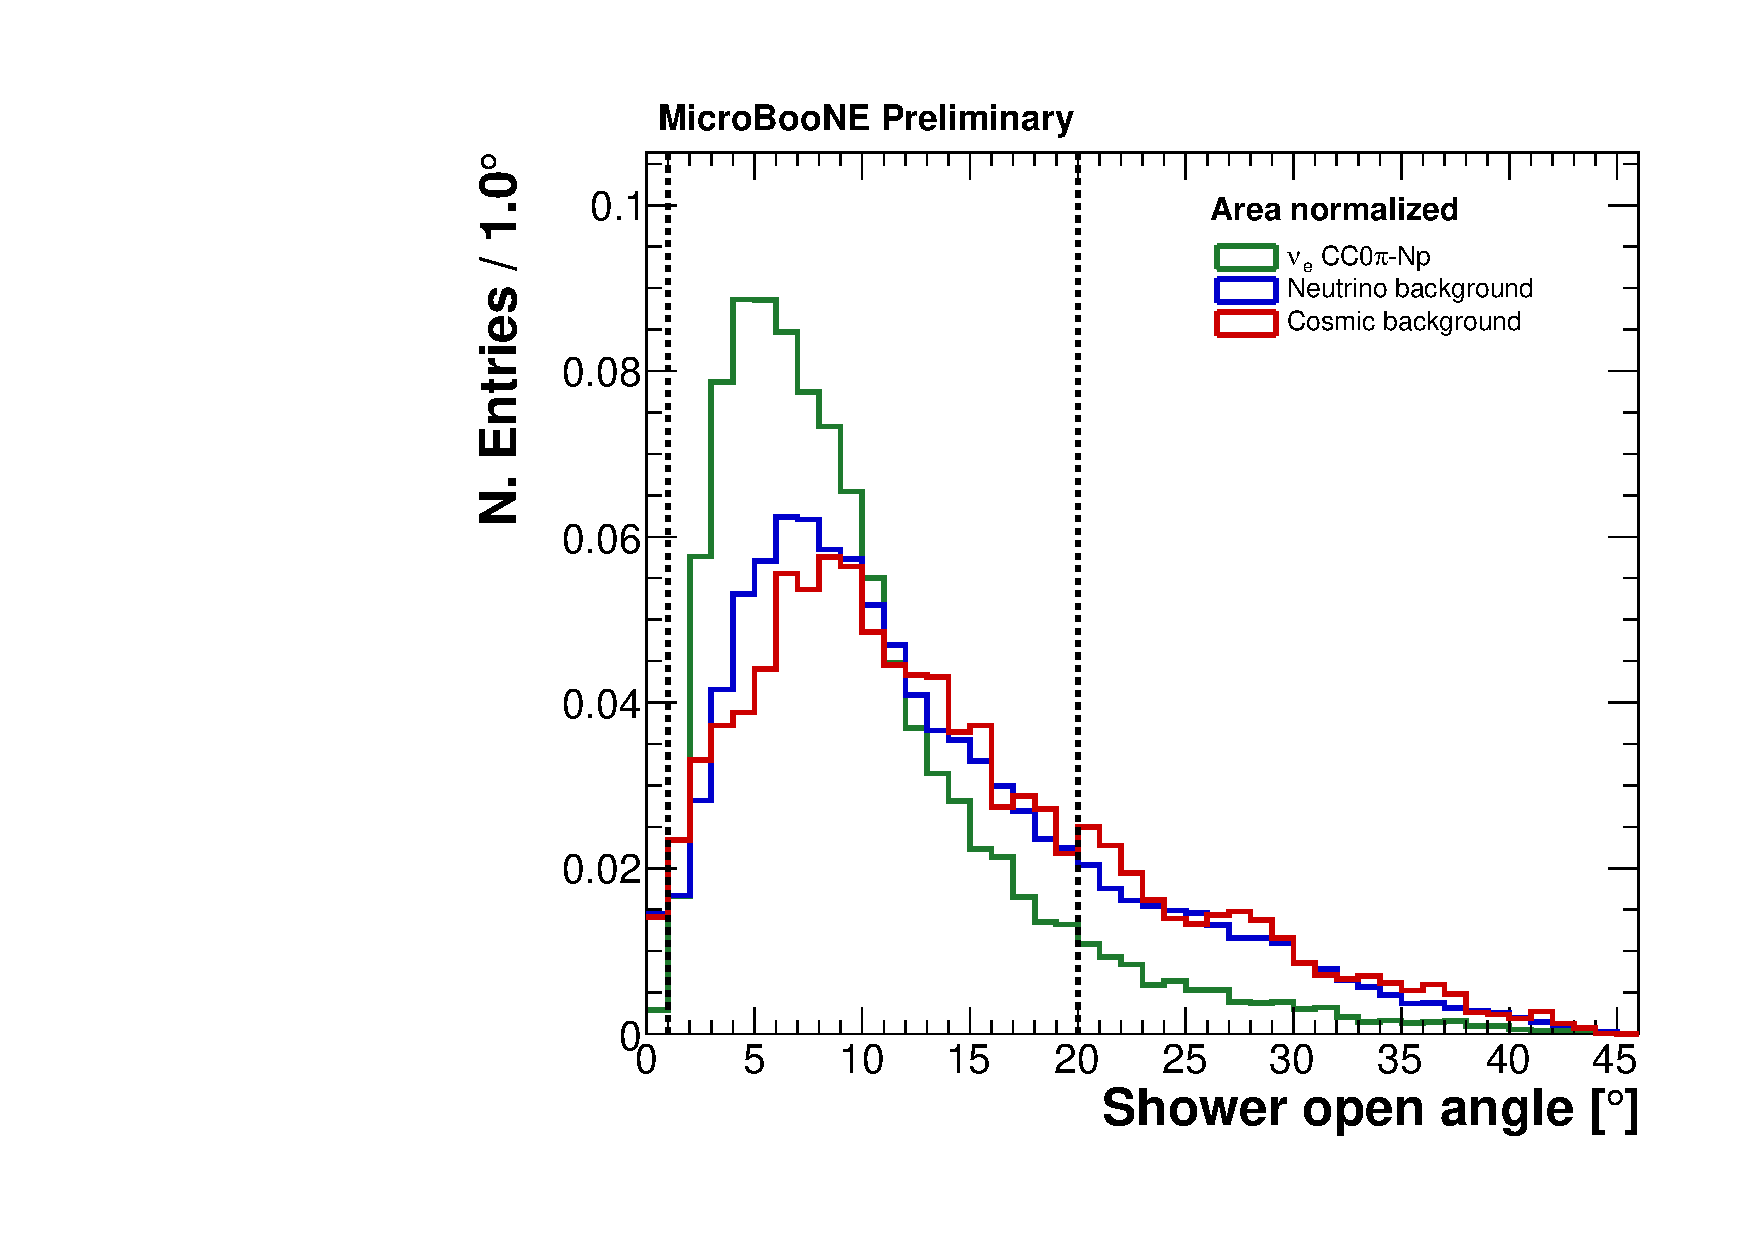
\includegraphics[width=\linewidth]{figures/h_shower_open_angle_norm.pdf}
%     \caption{Area normalised.} \label{fig:open_norm}
%   \end{subfigure}
%     \begin{subfigure}{0.49\textwidth}
%     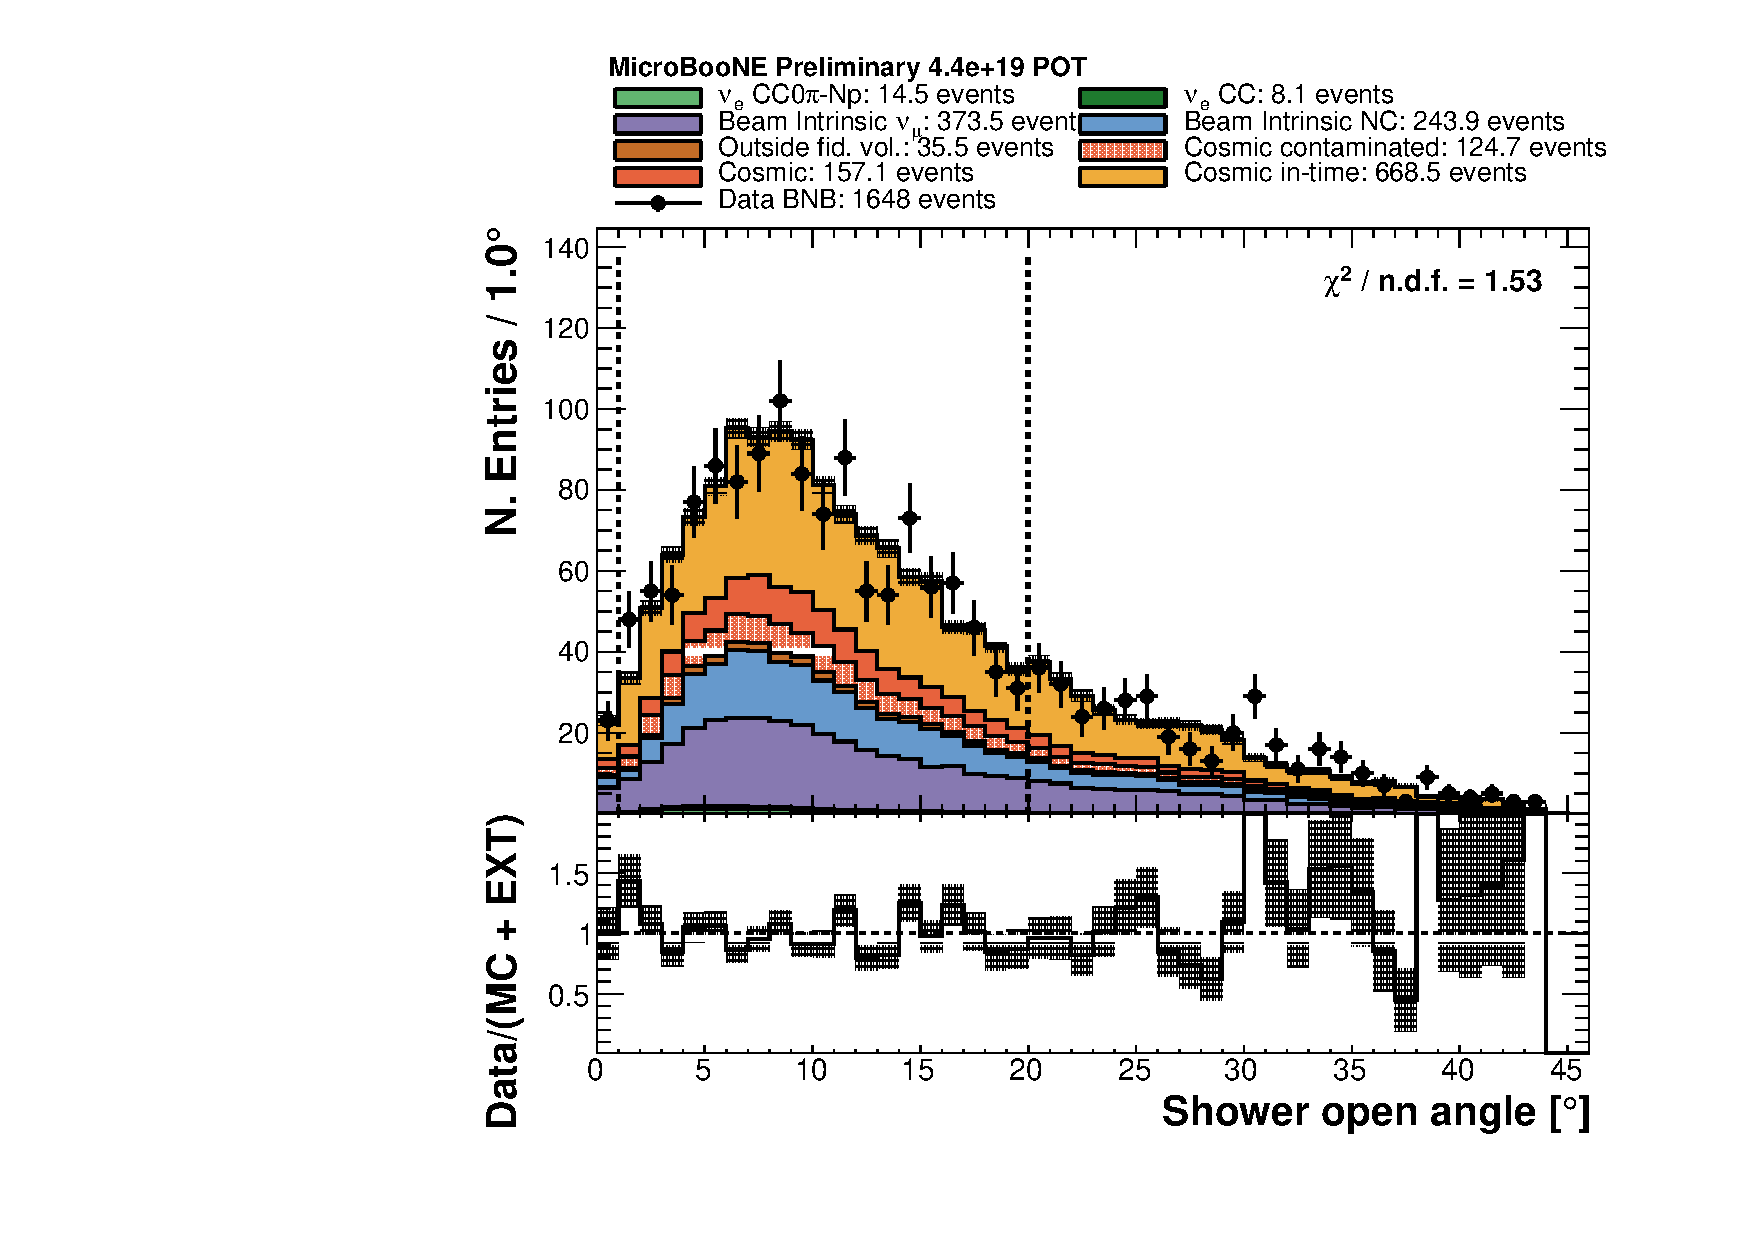
\includegraphics[width=\linewidth]{figures/h_shower_open_angle.pdf}
%     \caption{POT normalised.} \label{fig:open_pot}
%   \end{subfigure}
%   \caption{Area and POT normalised distributions of the opening angle $\beta$ of the most energetic shower.}
% \end{figure}

\begin{figure}[htbp]
\centering
  \begin{subfigure}{0.49\textwidth}
    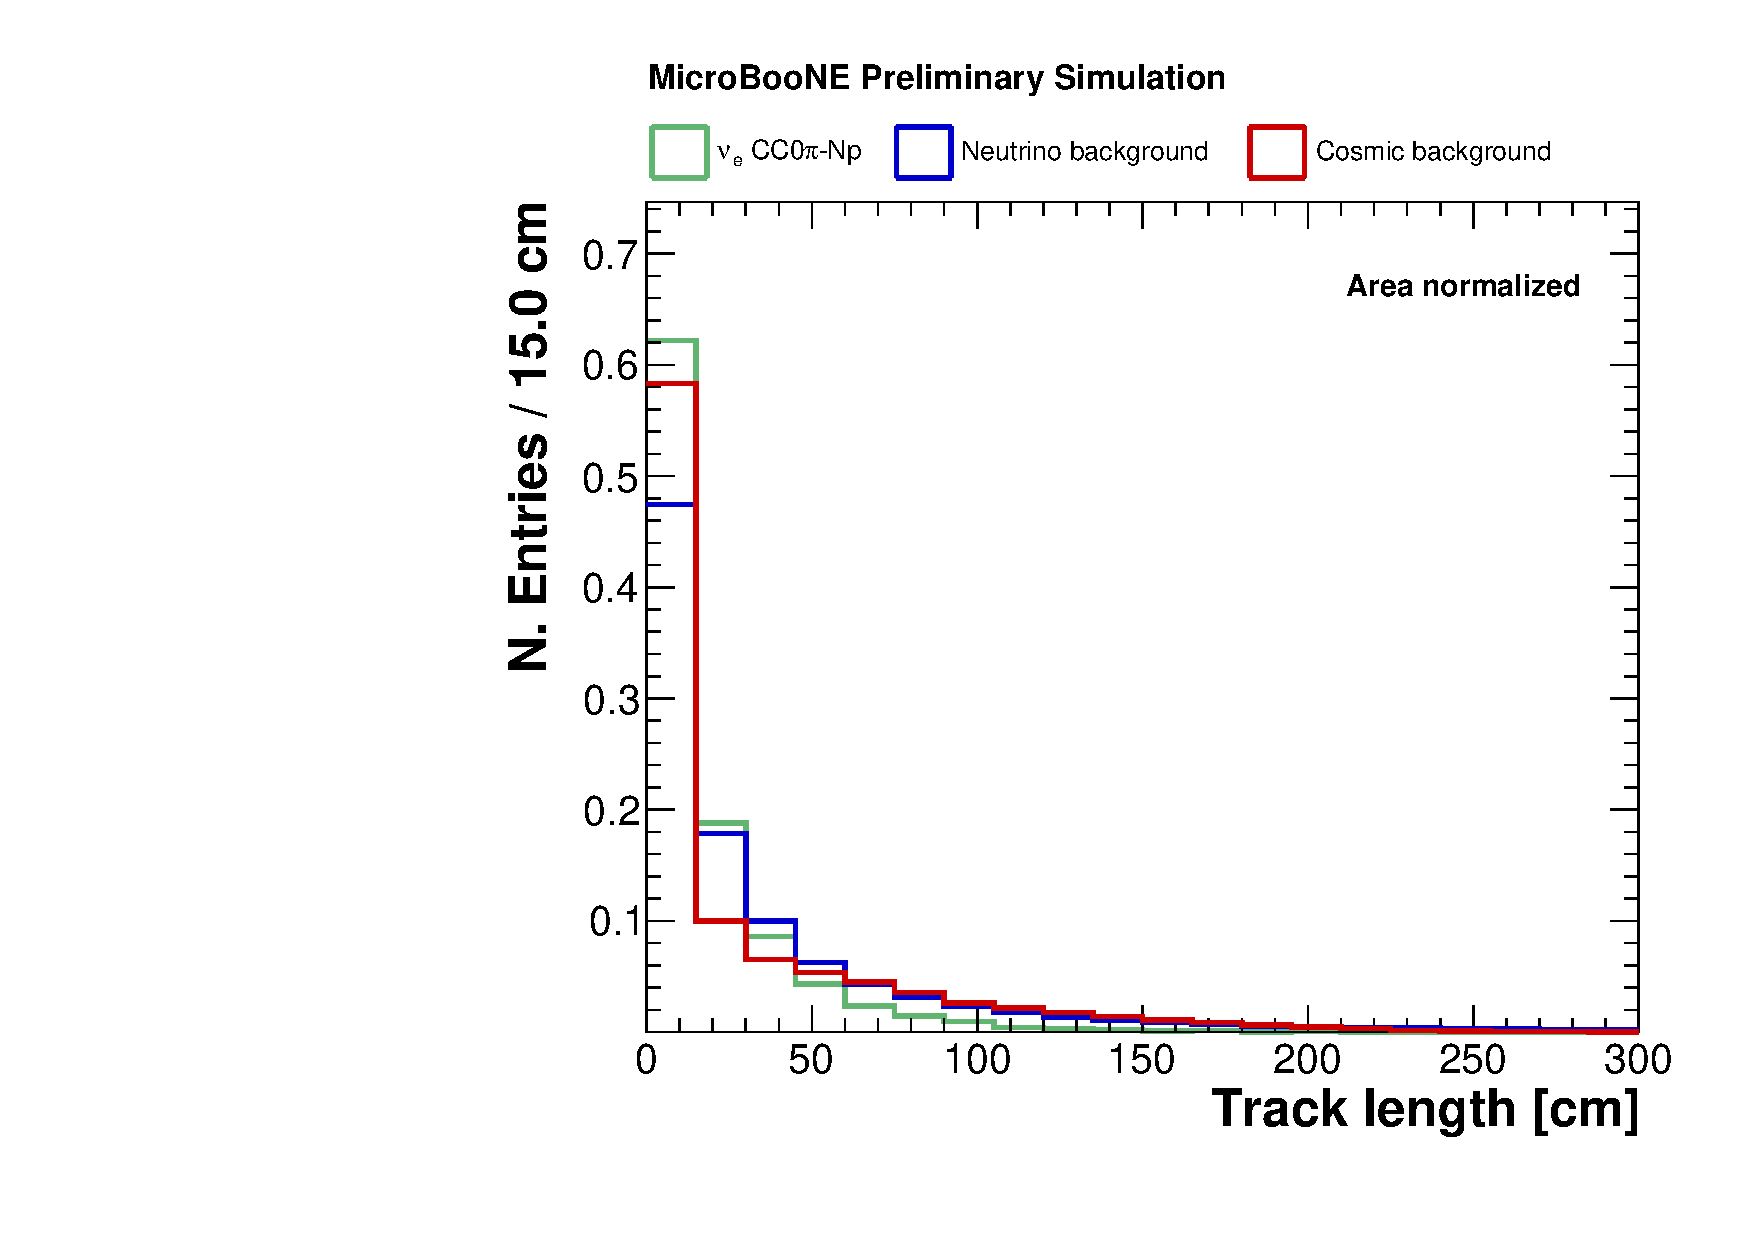
\includegraphics[width=\linewidth]{figures/h_track_length_norm.pdf}
    \caption{Area normalised.} \label{fig:length_norm}
  \end{subfigure}
  \begin{subfigure}{0.49\textwidth}
    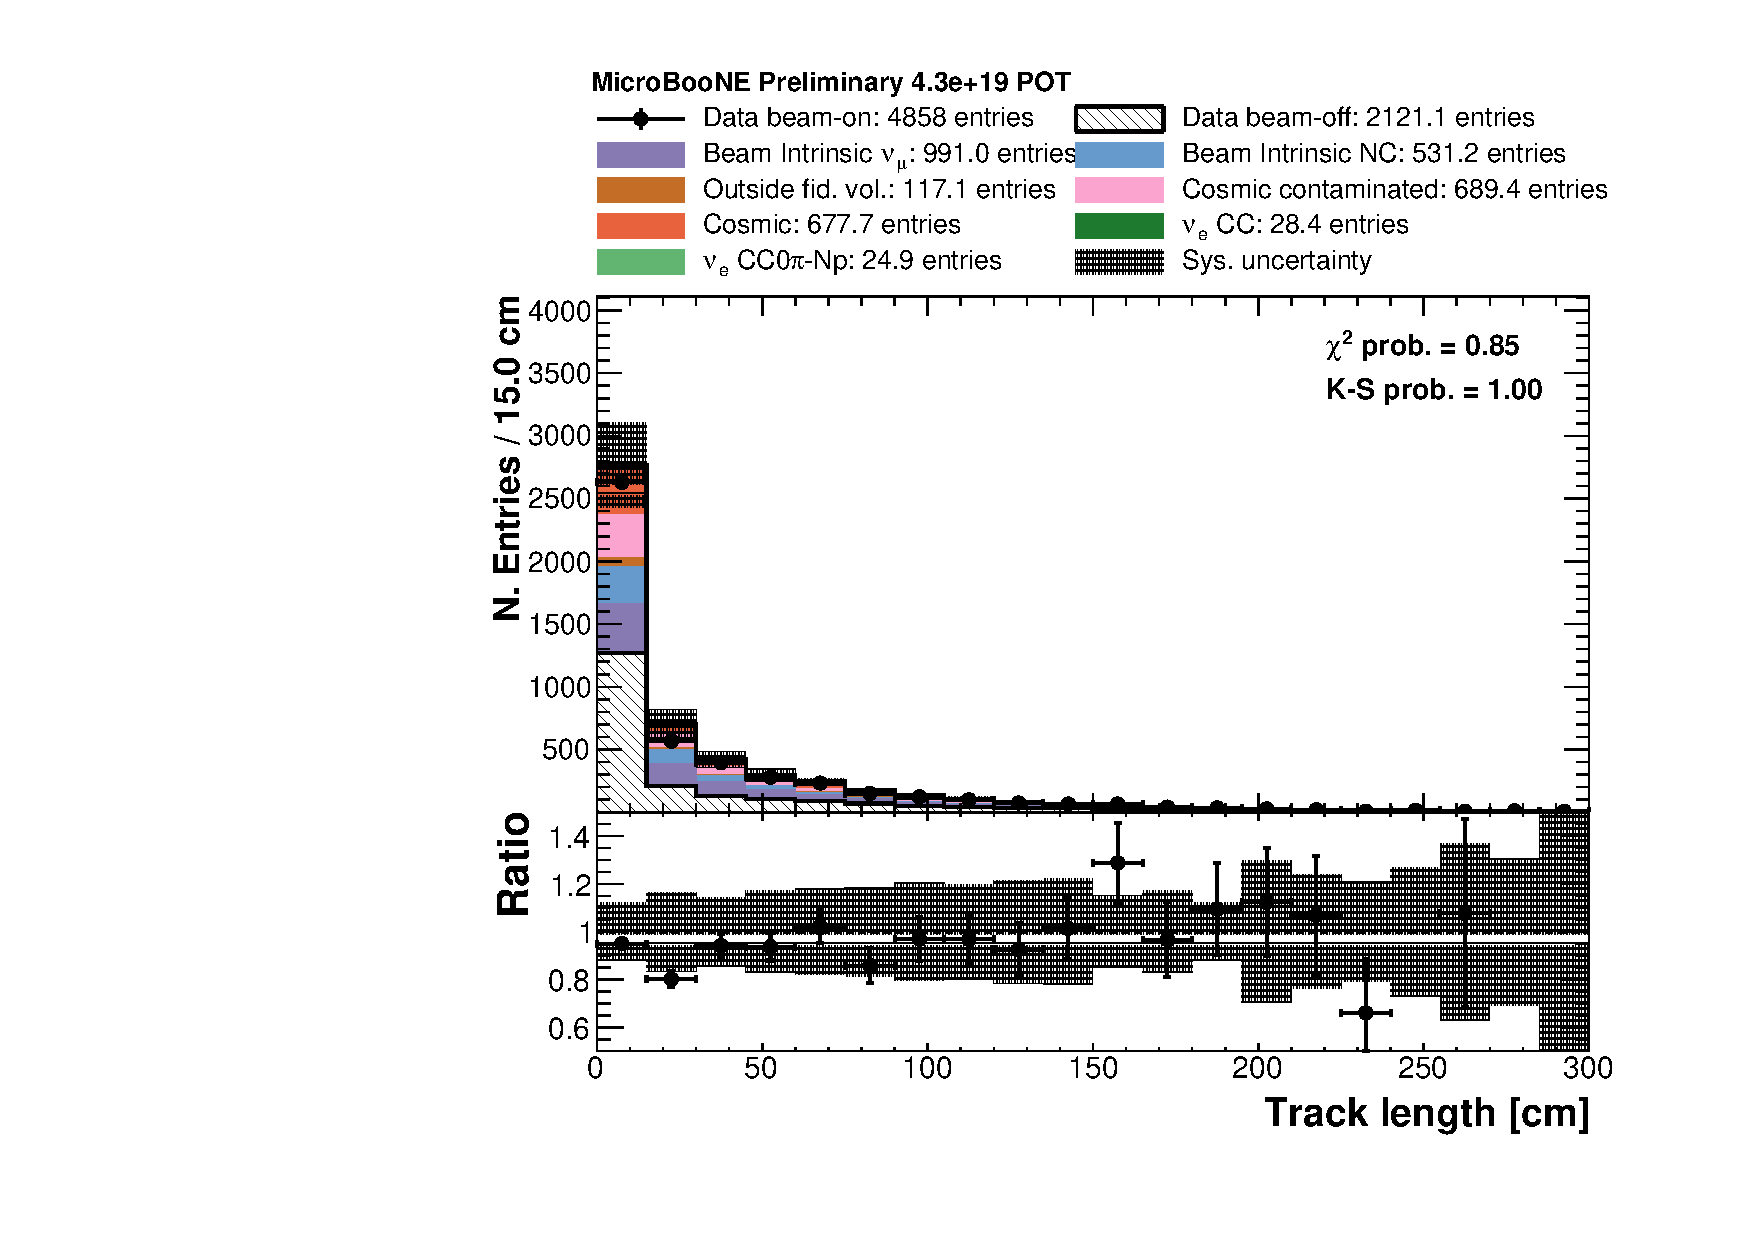
\includegraphics[width=\linewidth]{figures/h_track_length.pdf}
    \caption{POT normalised, event category.} \label{fig:length_pot}
  \end{subfigure}
  \begin{subfigure}{0.49\textwidth}
    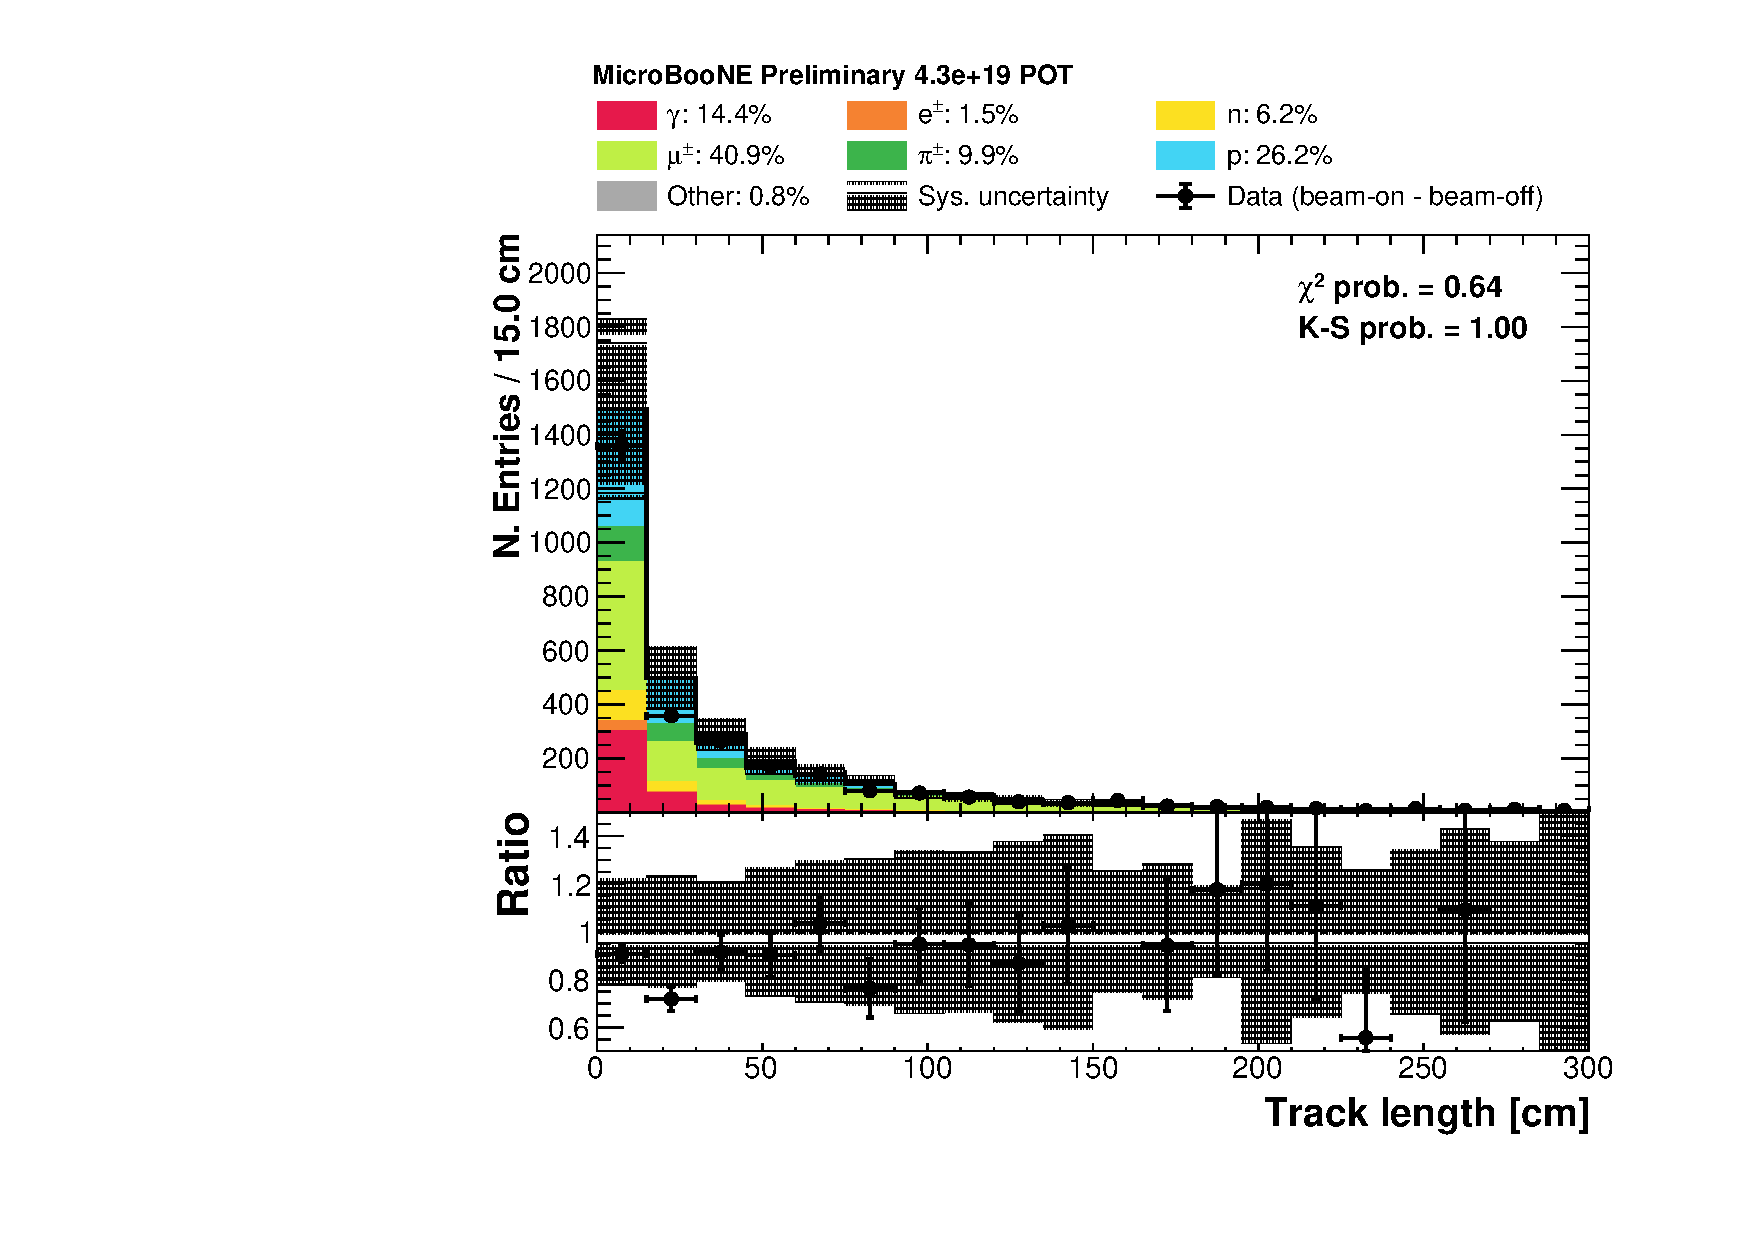
\includegraphics[width=\linewidth]{figures/h_track_length_pdg.pdf}
    \caption{POT normalised, generating particle.} \label{fig:length_pdg}
  \end{subfigure}
  \caption{Area and POT-normalised distributions of the length of each track in the event, classified according to the event category and to the primary particle generating the shower.}
\end{figure}